% !TEX encoding = UTF-8 Unicode
% !TEX TS-program = xelatex
\documentclass[12pt]{article}
\usepackage{tikz}
\usepackage{pgfplots}
\usetikzlibrary{calc, arrows, patterns,angles ,positioning,quotes}
\usetikzlibrary{decorations.markings}
\usetikzlibrary{arrows.meta}

\usepackage{tkz-euclide}
%==== Chinese Setting  ====== 

\input{E:/NCTUG2/TEX/LatexCodeTemplate/inputFile/Qheader.tex}
\includeonly{PicDB,PicCurrent,PicPoly,PicExponentAndLog, PicSequenceSeries,PicPermuationAndCombination,PicStatistics,PicTriangle,PicLineAndArea,,PicCircle,PicVector,PicDegree2,Pic3DDB}
%\includeonly{PicCurrent,PicDB}
%\includeonly{PicCurrent}

\begin{document}
    \chapter{待整理}

    % !TEX encoding = UTF-8 Unicode
% !TEX TS-program = xelatex

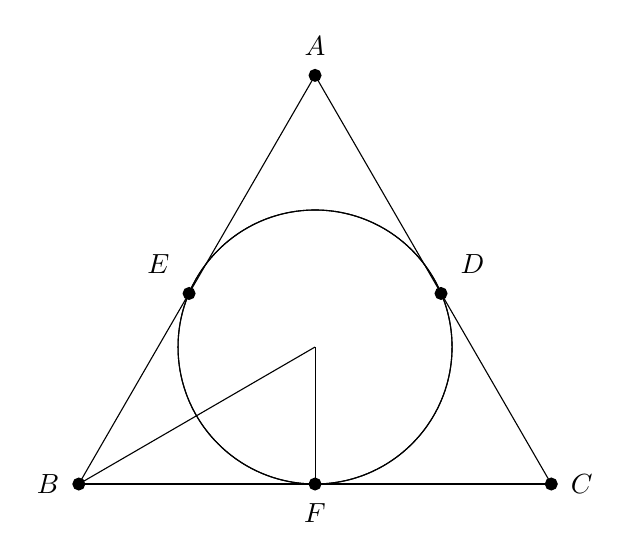
\begin{tikzpicture}
    \coordinate (cBPt) at (0,0);
    \coordinate (cCPt) at (6,0);
    \coordinate (cAPt) at (3.,5.19);
    \coordinate (cEPt) at (1.4,2.42);
    \coordinate (cFPt) at (3,0);
    \coordinate (cDPt) at (4.6,2.42);
    \draw(3.,1.74) circle (1.74);
    \draw (0.,0.)-- (6.,0.);
    \draw (6.,0.)-- (3.,5.19);
    \draw (3.,5.19)-- (0.,0.);
    \draw(3.,1.74) circle (1.74cm);
    \draw (0.,0.)-- (3.,1.74);
    \draw (3.,1.74)-- (3.,0.);
\foreach \v/\u/\t in 
{cAPt/90/$A$,
    cBPt/180/$B$,
    cCPt/0/$C$,
    cDPt/45/$D$,
    cEPt/135/$E$,
    cFPt/270/$F$
}
{
    \draw[ultra thick,fill] (\v) circle (1.5pt);
    \node[label=\u:\t] at (\v){};
};	    

    
\end{tikzpicture}
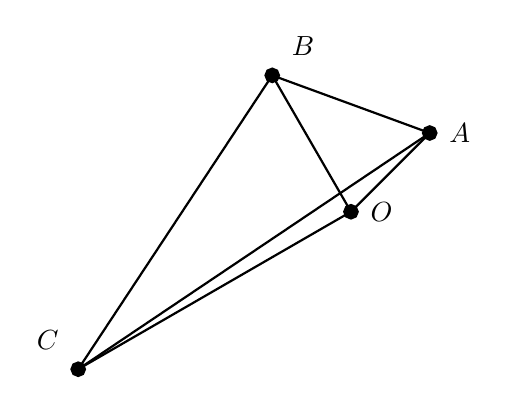
\begin{tikzpicture}
\coordinate (cOPt) at (0,0);
\coordinate (cAPt) at (45:{sqrt(2)});
\coordinate (cBPt) at (120:2);
\coordinate (cCPt) at (210:4);

\foreach \v/\u/\t in 
{cAPt/0/$A$,
    cBPt/45/$B$,
    cCPt/135/$C$,
    cOPt/0/$O$
}
{
    \draw[ultra thick,fill] (\v) circle (2pt);
    \node[label=\u:\t] at (\v){};
};	    

\draw[thick] (cAPt) -- (cBPt) -- (cCPt) circle;
\draw[thick] (cOPt) -- (cAPt) ;
\draw[thick] (cOPt) -- (cBPt) ;
\draw[thick] (cAPt) -- (cCPt) ;
\draw[thick] (cOPt) -- (cCPt) ;


\end{tikzpicture}

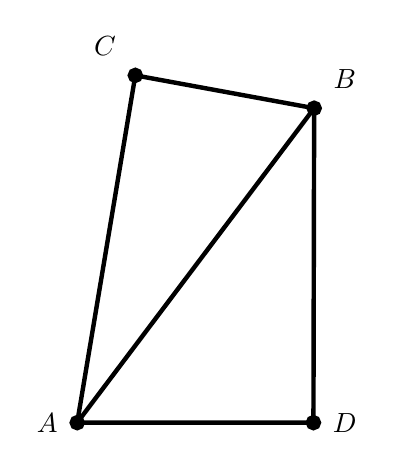
\begin{tikzpicture}

\coordinate (cAPt) at (0,0);
\coordinate (cBPt) at (53:5);
\coordinate (cCPt) at (80.5:{2*sqrt(5)});
\coordinate (cDPt) at (3,0);


\foreach \v/\u/\t in 
{cAPt/180/$A$,
    cBPt/45/$B$,
    cCPt/135/$C$,
    cDPt/0/$D$
}
{
    \draw[ultra thick,fill] (\v) circle (2pt);
    \node[label=\u:\t] at (\v){};
};	    

\draw[ultra thick] (cAPt) -- (cDPt) -- (cBPt)  -- (cCPt) -- (cAPt) circle;
\draw[ultra thick] (cAPt) -- (cBPt) ;

\end{tikzpicture}

    % !TEX encoding = UTF-8 Unicode
% !TEX TS-program = xelatex
\chapter{多項式圖形}


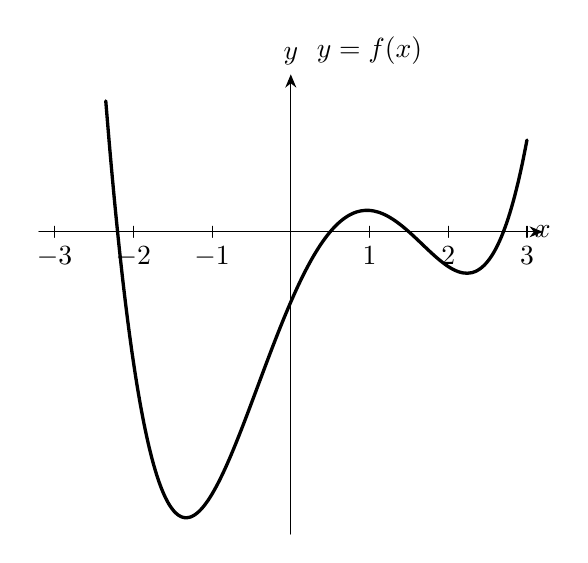
\begin{tikzpicture}[line cap=round,line join=round,x=1.0cm,y=0.2cm]
\draw[-{Stealth[scale=1,angle'=45]},color=black] (-3.2,0.) -- (3.2,0)  node[] {$x$};
\draw[-{Stealth[scale=1,angle'=45]},color=black] (0,-19.2) -- (0,10)  node[above] {$y$};

\draw[line width=1.2pt,smooth,samples=100,domain=-2.35:3] plot(\x,{1*(\x +2.2 )*(\x -0.5) *(\x - 1.5)*(\x -2.7) }) ;
\node [above ] at (1,10){ $y = f(x)$};
%畫上
\foreach \v in 
{-3,-2,-1,1,2,3}
{
    \draw[shift={(\v,0)},color=black] (0pt,2pt) -- (0pt,-2pt) node[below] { $\v$};
};

%\draw[ultra thick,fill] (1.5,-2) circle (0.8pt) node [ below] {$(1.5,-2)$};

\end{tikzpicture}

    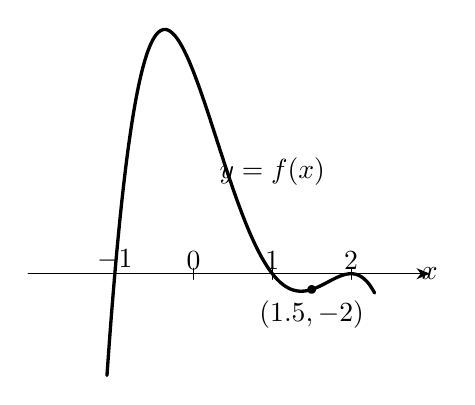
\begin{tikzpicture}[line cap=round,line join=round,x=1.0cm,y=0.1cm]
\draw[-{Stealth[scale=1,angle'=45]},color=black] (-2.1,0.) -- (3,0.)  node[] {$x$};

\draw[line width=1.2pt,smooth,samples=100,domain=-1.1:2.3] plot(\x,{-6.4*(\x +1)*(\x -1) *(\x - 2)*(\x -2) }) ;
\node [above ] at (1,10){ $y = f(x)$};
%畫上
\foreach \v in 
{-1,0,1,2}
{
    \draw[shift={(\v,0)},color=black] (0pt,2pt) -- (0pt,-2pt) node[above] { $\v$};
};

\draw[ultra thick,fill] (1.5,-2) circle (0.8pt) node [ below] {$(1.5,-2)$};

\end{tikzpicture}

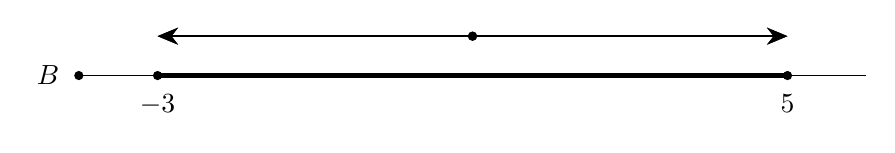
\begin{tikzpicture}
\coordinate (cLineL) at (-4, 0);
\coordinate (cLineR) at (6, 0);
\coordinate (cAL) at (-3,0);
\coordinate (cAR) at (5,0);

\draw  (cLineL) -- (cLineR);
\draw[ultra thick]  (cAL) -- (cAR);

\begin{scope}[shift={(0,0.5)}]
\def\Bradius{4}
\coordinate (cBC) at (1, 0);
\coordinate (cBR) at (1 + \Bradius, 0);
\coordinate (cBL) at (1 - \Bradius, 0);
\draw [-{Stealth[scale=1.3,angle'=45]},semithick]  (cBC) -- (cBR);
\draw [-{Stealth[scale=1.3,angle'=45]},semithick]  (cBC) -- (cBL);
\draw[ultra thick,fill] (cBC) circle (0.8pt);
\end{scope}


\foreach \v in 
{   1
}
{
    \begin{scope}[shift={(0,0.5)}]
    \def\Bradius{4}
    \coordinate (cBC) at (\v, 0);
    \coordinate (cBR) at (\v + \Bradius, 0);
    \coordinate (cBL) at (\v - \Bradius, 0);
    \draw [-{Stealth[scale=1.3,angle'=45]},semithick]  (cBC) -- (cBR);
    \draw [-{Stealth[scale=1.3,angle'=45]},semithick]  (cBC) -- (cBL);
    \draw[ultra thick,fill] (cBC) circle (0.8pt);
    \end{scope}
};

\foreach \v/\u/\t in 
{   cAL/270/$-3$,
    cAR/270/$5$,
    cLineL/180/$B$
}
{
    \draw[ultra thick,fill] (\v) circle (0.8pt);
    \node[label=\u:\t] at (\v){};
};

\end{tikzpicture}

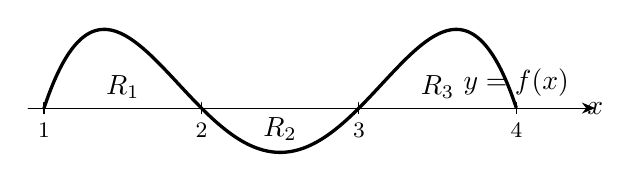
\begin{tikzpicture}[line cap=round,line join=round,x=2cm,y=1cm]
\draw[-{Stealth[scale=1,angle'=45]},color=black] (0.9,0.) -- (4.5,0.)  node[] {$x$};
%\draw[-{Stealth[scale=1,angle'=45]},color=black] (0.,-4.) -- (0.,1.5) node[above] {$y$};
\foreach \x in {1,2,3,4}
\draw[shift={(\x,0)},color=black] (0pt,2pt) -- (0pt,-2pt) node[below] {\footnotesize $\x$};
\draw[line width=1.2pt,smooth,samples=100,domain=1:4] plot(\x,{-1*((\x -1)*(\x-2)*(\x-3)*(\x-4))}) node [above ] { $y = f(x)$};
\node [ above ] at (1.5,0) {$R_1$};
\node [ below ] at (2.5,0) {$R_2$};
\node [ above ] at (3.5,0) {$R_3$};
\end{tikzpicture}

\begin{tikzpicture}[line cap=round,line join=round,x=2cm,y=1cm]
\draw[-{Stealth[scale=1,angle'=45]},color=black] (0.9,0.) -- (2.5,0.)  node[] {$x$};
\draw[-{Stealth[scale=1,angle'=45]},color=black] (0.,-4.) -- (0.,1.5) node[above] {$y$};
\foreach \x in {1,2,3,4}
\draw[shift={(\x,0)},color=black] (0pt,2pt) -- (0pt,-2pt) node[below] {\footnotesize $\x$};
\draw[line width=1.2pt,smooth,samples=100,domain=-0.1:2.1] plot(\x,{3*((\x )*(\x-2))}) node [above ] { $y = f(x)$};

\draw[ultra thick,fill] (1,0) circle (1pt) node [ above left] {$B(-1,0)$};
\draw[ultra thick,fill] (2,0) circle (1pt) node [ above ] {$A(0,0)$};
\draw[ultra thick,fill] (3,-3) circle (1pt) node [ below] {$C(1,-3)$};

\end{tikzpicture}

\begin{tikzpicture}[line cap=round,line join=round,x=0.5cm,y=0.5cm]
\draw[-{Stealth[scale=1,angle'=45]},color=black] (0,0.) -- (10,0.)  node[] {$x$};
%\foreach \x in {-3,-2,-1,1,2}
%\draw[shift={(\x,0)},color=black] (0pt,2pt) -- (0pt,-2pt) node[below] {\footnotesize $\x$};
\draw[-{Stealth[scale=1,angle'=45]},color=black] (0.,0) -- (0.,10) node[above] {$y$};
%\foreach \y in {1,2}
%\draw[shift={(0,\y)},color=black] (2pt,0pt) -- (-2pt,0pt) node[left] { $\y$};
\draw[line width=1.2pt,smooth,samples=100,domain=3:7] plot(\x,{0.33*((\x -5 )*(\x-5) * (\x-5))+\x}) node [above ] { $y = f(x)$};
%畫上
\foreach \v in 
{5}
{
    \draw[shift={(\v,0)},color=black] (0pt,2pt) -- (0pt,-2pt) node[below] { $\v$};
};
\end{tikzpicture}

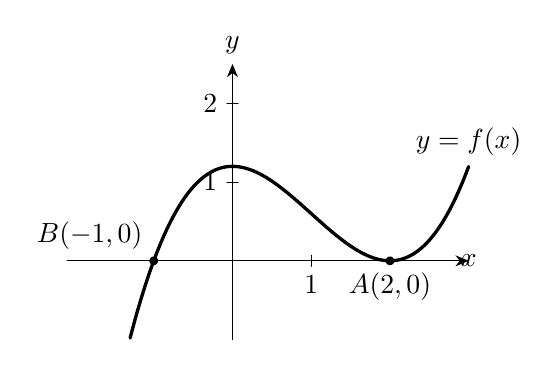
\begin{tikzpicture}[line cap=round,line join=round,x=1.0cm,y=1cm]
\draw[-{Stealth[scale=1,angle'=45]},color=black] (-2.1,0.) -- (3,0.)  node[] {$x$};
%\foreach \x in {-3,-2,-1,1,2}
%\draw[shift={(\x,0)},color=black] (0pt,2pt) -- (0pt,-2pt) node[below] {\footnotesize $\x$};
\draw[-{Stealth[scale=1,angle'=45]},color=black] (0.,-1.) -- (0.,2.5) node[above] {$y$};
\foreach \y in {1,2}
\draw[shift={(0,\y)},color=black] (2pt,0pt) -- (-2pt,0pt) node[left] { $\y$};

%\draw[color=black] (0pt,-10pt) node[] {\footnotesize $0$};
%\clip(-3.1,-15.) rectangle (2.3,35.);
\draw[line width=1.2pt,smooth,samples=100,domain=-1.3:3] plot(\x,{0.3*((\x -2 )*(\x-2) * (\x+1))}) node [above ] { $y = f(x)$};
%畫上
\foreach \v in 
{1}
{
    \draw[shift={(\v,0)},color=black] (0pt,2pt) -- (0pt,-2pt) node[below] { $\v$};
};


\draw[ultra thick,fill] (-1,0) circle (0.8pt) node [ above left] {$B(-1,0)$};
\draw[ultra thick,fill] (2,0) circle (0.8pt) node [ below] {$A(2,0)$};

\end{tikzpicture}

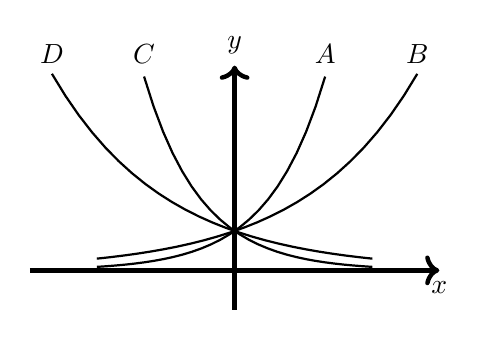
\begin{tikzpicture}[scale=.5]
\draw[ultra thick, ->] (-5.2,0) -- (5.2,0) node[below] {$x$};
\draw[ultra thick, ->] (0,-1) -- (0,5.2) node[above] {$y$};
%        \draw[very thin,color=gray] (-5,-1) grid (5,5);
\draw[thick, color=black, domain=-3.5:4.64] plot (\x,{2^(\x/2)});
\draw[thick, color=black, domain=-3.5:2.3] plot (\x,{2^(\x)});
\draw[thick, color=black, domain=-4.64:3.5] plot (\x,{2^(-\x/2)});
\draw[thick, color=black, domain=-2.3:3.5] plot (\x,{2^(-\x)});
\node[above] at (4.64, 5) {$B$};
\node[above] at (2.3, 5) {$A$};
\node[above] at (-4.64, 5) {$D$};
\node[above] at (-2.3, 5) {$C$};

\end{tikzpicture}

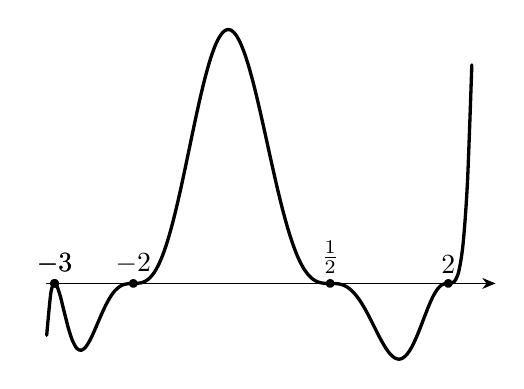
\begin{tikzpicture}[line cap=round,line join=round,x=1.0cm,y=0.1cm]
\draw[-{Stealth[scale=1,angle'=45]},color=black] (-3.1,0.) -- (2.6,0.);
%\foreach \x in {-3,-2,-1,1,2}
%\draw[shift={(\x,0)},color=black] (0pt,2pt) -- (0pt,-2pt) node[below] {\footnotesize $\x$};
%\draw[->,color=black] (0.,-15.) -- (0.,35.);
%\foreach \y in {-10,10,20,30}
%\draw[shift={(0,\y)},color=black] (2pt,0pt) -- (-2pt,0pt) node[left] {};

%\draw[color=black] (0pt,-10pt) node[] {\footnotesize $0$};
%\clip(-3.1,-15.) rectangle (2.3,35.);
\draw[line width=1.2pt,smooth,samples=100,domain=-3.1:2.3] plot(\x,{0.01*(2.0*(\x)-1.0)^(3.0)*((\x)^(2.0)-4.0)^(3.0)*((\x)+3.0)^(2.0)});


\foreach \v in 
{   -3,-2,2,-3
}
{
    \draw[ultra thick,fill] (\v,0) circle (0.8pt);
    \node[above] at (\v,0){$\v$};
};

\draw[ultra thick,fill] (0.5,0) circle (0.8pt);
\node[above] at (0.5,0){$\frac{1}{2}$};
\end{tikzpicture}
\def\FunctionG(#1){+((#1) + 0.5)*((#1) -2)* ((#1) -4)}%
\begin{tikzpicture}
\begin{axis}[
%axis y line=center,
%axis x line=middle, 
%axis on top=true,
xmin=-2,
xmax=6,
ymin=-5,
ymax=24,
height=6.0cm,
width=8.0cm,
%grid,
%xtick={-1,...,5},
%ytick={-40,-32,...,40},
hide y axis,
hide x axis,
]
\addplot [domain=-1.5:5, samples=50, mark=none, ultra thick] {\FunctionG(x)};
\draw[line width=1.7pt,-{Stealth[scale=1,angle'=45]}] (axis cs:-2,0 ) -- (axis cs:5.5,0) node [] {$x$};
\draw[line width=1.7pt,-{Stealth[scale=1,angle'=45]}] (axis cs:0,-5 ) -- (axis cs:0,20) node [left] {$y$};
\node [left] at (axis cs: 3.6,10) {$y=f(x)$};

\end{axis}
\end{tikzpicture}
\def\FunctionF(#1){+((#1) + 0.5)*((#1) -2)* ((#1) -4)}%
\begin{tikzpicture}
\begin{axis}[
%axis y line=center,
%axis x line=middle, 
%axis on top=true,
xmin=-2,
xmax=6,
ymin=-5,
ymax=24,
height=6.0cm,
width=8.0cm,
%grid,
%xtick={-1,...,5},
%ytick={-40,-32,...,40},
hide y axis,
hide x axis,
]
\addplot [domain=-1.5:5, samples=50, mark=none, ultra thick] {\FunctionF(x)};
\draw[line width=1.7pt,-{Stealth[scale=1,angle'=45]}] (axis cs:-2,0 ) -- (axis cs:5.5,0) node [] {$x$};
\draw[line width=1.7pt,-{Stealth[scale=1,angle'=45]}] (axis cs:0,-5 ) -- (axis cs:0,20) node [left] {$y$};
\node [left] at (axis cs: 3.6,10) {$y=f(x)$};
%\draw[ultra thick] (axis cs:-1,0) circle (2pt);
%\draw[ultra thick] (axis cs: 2,0) circle (2pt);
%\draw[ultra thick] (axis cs: 4,0) circle (2pt);
%\node [below] at (axis cs: -1,0) {$-1$};
%\node [below] at (axis cs: 2,0) {$2$};
%\node [below] at (axis cs: 4,0) {$4$};
\end{axis}
\end{tikzpicture}

\section{勘根}
    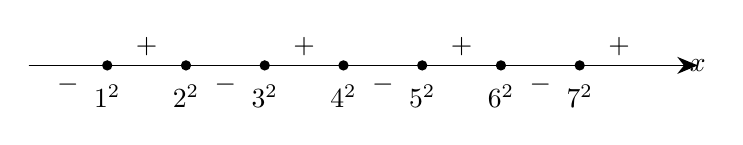
\begin{tikzpicture}[scale=1]
\draw[-{Stealth[scale=1.3,angle'=45]},semithick] (0,0) -- (8.5,0) node[] {$x$};
\foreach \v in 
{1,2,3,4,5,6,7}
{
    \draw[ultra thick,fill] (\v,0) circle (1pt);
    \node[label={270:$\v ^2$}] at (\v,0){};
};
\foreach \v/\u in 
{0/1,2/3,4/5,6/7}
{
    \draw [semithick] (\v,0) -- (\u,0) node [midway, below] {$-$};
};
\foreach \v/\u in 
{1/2,3/4,5/6,7/8}
{
    \draw [semithick] (\v,0) -- (\u,0) node [midway, above] {$+$};
};

\end{tikzpicture}

    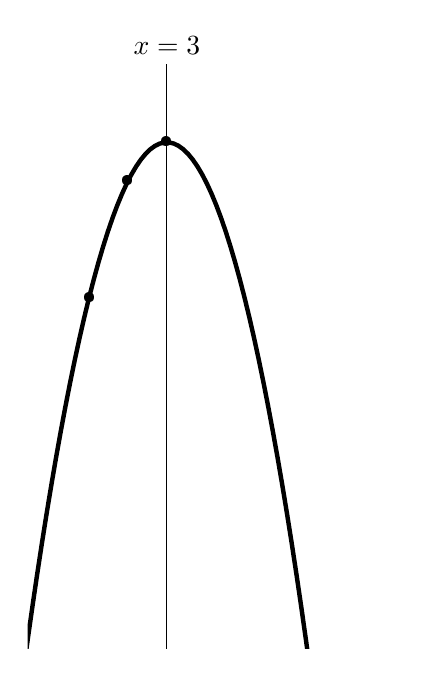
\begin{tikzpicture}
\makeatletter
\tikzset{
    nomorepostaction/.code=\makeatletter\let\tikz@postactions\pgfutil@empty, % From http://tex.stackexchange.com/questions/3184/applying-a-postaction-to-every-path-in-tikz/5354#5354
    my axis/.style={
        postaction={
            decoration={
                markings,
                mark=at position 1 with {
                    \arrow[ultra thick]{latex}
                }
            },
            decorate,
            nomorepostaction
        },
        thin,
        -, % switch off other arrow tips
        every path/.append style=my axis % this is necessary so it works both with "axis lines=left" and "axis lines=middle"
    }
}
\makeatother
\pgfplotsset{ticks=none}
\begin{axis}[
unit vector ratio*=1 1 1,
axis lines = middle,
axis line style = {my axis},
hide y axis,
hide x axis,
width=11cm,
xlabel={$x$},
ylabel={$y$},
ymax =12,
ymin =-4,
xmax = 10,
xmin = 
]
%Below the red parabola is defined
\addplot [
domain=-3:9, 
samples=100, 
color=black,ultra thick
]
{-x*x+6*x};
%\addlegendentry{$\$}
%Here the blue parabloa is defined
\draw (axis cs:3,-10) -- (axis cs:3,11) node [above] {$x=3$};
\node at (axis cs:1, 5) {\textbullet};
\node at (axis cs:2, 8) {\textbullet};
\node at (axis cs:3, 9) {\textbullet};
%    \foreach \Point in {(axis cs:1, 5), (axis cs:2,8), (axis cs:3,9)}{
%    \node at \Point {\textbullet};
%};

\end{axis}
\end{tikzpicture}

\pgfmathdeclarefunction{myfunct}{1}{%
    \pgfmathparse{-1*(#1+0.5)*(#1-1.5)}%
}
\begin{tikzpicture}
%\pgfplotsset{ticks=none}
\begin{axis}[
unit vector ratio*=1 1 1,
axis lines = middle,
axis line style = {-{Stealth[scale=1.3,angle'=45]}},
%hide y axis,
%hide x axis,
width=7cm,
xlabel={$x$},
ylabel={$y$},
xtick={-2,-1,...,3},
ymax =2.5,
ymin =-4.5,
xmax = 3.5,
xmin = -2.5
]
%Below the red parabola is defined
\addplot[samples=100,domain=-2:3] {myfunct(x)};
%\addlegendentry{$\$}
%Here the blue parabloa is defined



\end{axis}
\end{tikzpicture}

    \pgfmathdeclarefunction{myfunct2}{1}{%
    \pgfmathparse{-1*(#1-3)^2+2}%
}
\begin{tikzpicture}
%\pgfplotsset{ticks=none}
\begin{axis}[
unit vector ratio*=1 1 1,
axis lines = middle,
axis line style = {-{Stealth[scale=1.3,angle'=45]}},
hide y axis,
hide x axis,
width=7cm,
xlabel={$x$},
ylabel={$y$},
xtick={-2,-1,...,3},
ymax =2.5,
ymin =-4.5,
xmax = 8,
xmin = -2
]
%Below the red parabola is defined
\addplot[samples=100,domain=-2:8] {myfunct2(x)};
%\addlegendentry{$\$}
%Here the blue parabloa is defined
\pgfplotsinvokeforeach{1,2,3,4,5}{ 
    %    \addplot coordinates { (#1,0) (#1,{myfunct2(#1)}) }; \node[above=5pt] at (axis cs:#1,{myfunct2(#1)}) {\pgfmathprint{myfunct2(#1)}}; }
    
    \node at (axis cs:#1, {myfunct2(#1)}) {\textbullet };
    \node at (axis cs:#1, {myfunct2(#1)}) { $(#1, f(#1))$};
}

\end{axis}
\end{tikzpicture}
    % !TEX encoding = UTF-8 Unicode
% !TEX TS-program = xelatex

\chapter{指數對數圖形}

        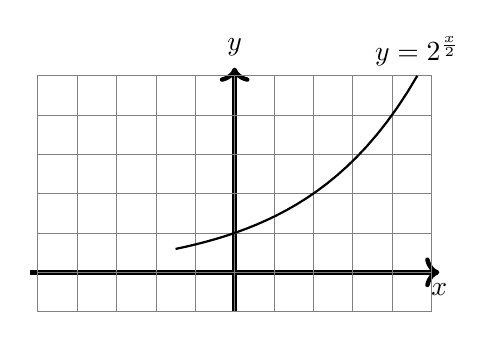
\begin{tikzpicture}[scale=.5]
\draw[ultra thick, ->] (-5.2,0) -- (5.2,0) node[below] {$x$};
\draw[ultra thick, ->] (0,-1) -- (0,5.2) node[above] {$y$};
\draw[very thin,color=gray] (-5,-1) grid (5,5);
\draw[thick, color=black, domain=-1.5:4.64] plot (\x,{2^(\x/2)});
\node[above] at (4.64, 5) {$y={2}^{\frac{x}{2} }$};
\end{tikzpicture}

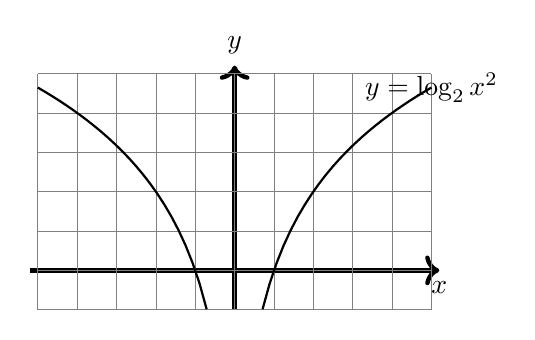
\begin{tikzpicture}[scale=.5]
\draw[ultra thick, ->] (-5.2,0) -- (5.2,0) node[below] {$x$};
\draw[ultra thick, ->] (0,-1) -- (0,5.2) node[above] {$y$};
\draw[very thin,color=gray] (-5,-1) grid (5,5);
\draw[thick, color=black, domain=0.71:5] plot (\x, {log10(\x)/log10(sqrt(2))});
\draw[thick, color=black, domain=-5:-0.71] plot (\x, {log10(-\x)/log10(sqrt(2))});
\node[] at (5,4.64 ) {$y=\log_{2} x^2$};
\end{tikzpicture}

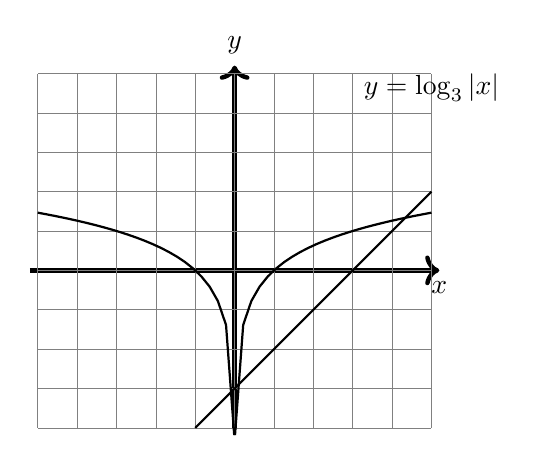
\begin{tikzpicture}[scale=.5]
\draw[ultra thick, ->] (-5.2,0) -- (5.2,0) node[below] {$x$};
\draw[ultra thick, ->] (0,-4) -- (0,5.2) node[above] {$y$};
\draw[very thin,color=gray] (-5,-4) grid (5,5);
\draw[thick, color=black, domain=0.01:5] plot (\x, {log10(\x)/log10(3)});
\draw[thick, color=black, domain=-5:-0.01] plot (\x, {log10(-\x)/log10(3)});
\draw[thick] (-1,-4) -- (5,2);

\node at (5,4.64) {$y=\log_{3} \left| x \right|$};
\end{tikzpicture}


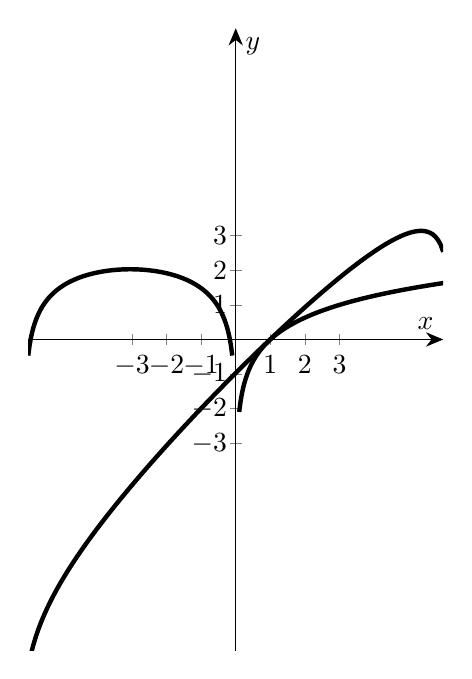
\begin{tikzpicture}[scale=1.0]
\pgfmathdeclarefunction{exxA}{0}{%
    \pgfmathparse{ln(x)/ln(3)}%
}
\pgfmathdeclarefunction{exxB}{0}{%
    \pgfmathparse{ln(-x)/ln(3)}%
}
\pgfmathdeclarefunction{polyA}{0}{%
    \pgfmathparse{x-3}%
}
\begin{axis}[
unit vector ratio*=1 1 1,
axis lines = middle,
axis line style =  {-{Stealth[scale=1.3,angle'=45]}},
width=11cm,
xlabel={$x$},
ylabel={$y$},
domain=-6:6,
ymin=-9,
ymax=9,
xmin=-6,
xmax=+6,
xtick={-3,-2,-1,0,1,2,3},
ytick={-3,-2,-1,0,1,2,3},
samples=160,
stack plots=y,
y tick label style={, xshift=0.25em}
]
%\draw[thick] (axis cs:-1,-1) -- (axis cs:-1,3);

\addplot+[black,ultra thick,mark=none,stack plots=y, domain=0.1:6] {exxA};
\addplot+[black,ultra thick,mark=none,stack plots=y, domain=-6:-0.1] {exxB};
%\node at (axis cs:-1, -1.5) {$x=-1$};
\addplot+[black,ultra thick,mark=none,stack plots=y, domain=-6:6] {polyA};

\end{axis}
\end{tikzpicture}

\begin{tikzpicture}[scale=1.0]
\pgfmathdeclarefunction{polyAAA}{0}{%
    \pgfmathparse{ln(x)/ln(0.5)-0.7}%
}
\begin{axis}[
unit vector ratio*=1 1 1,
axis lines = middle,
axis line style =  {-{Stealth[scale=1.3,angle'=45]}},
width=11cm,
xlabel={$x$},
ylabel={$y$},
domain=-2:14,
ymin=-2,
ymax=+3,
xmin=-1.5,
xmax=+3,
xtick={-1,0,1,2},
ytick={-1,0,1,2},
samples=160,
stack plots=y,
y tick label style={, xshift=0.25em}
]
%\draw[thick] (axis cs:-1,-1) -- (axis cs:-1,3);

\addplot+[black,ultra thick,mark=none,stack plots=y, domain=-0.9:3] {polyAAA};
%\node at (axis cs:-1, -1.5) {$x=-1$};

\end{axis}
\end{tikzpicture}

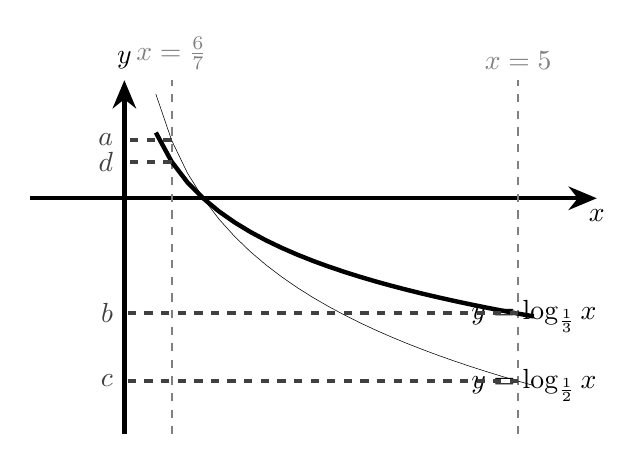
\begin{tikzpicture}[yscale=1, xscale=1]
\coordinate (A) at (0.6,0.74);
\coordinate (Al) at (0,0.74);
\coordinate (B) at (5,-1.46);
\coordinate (Bl) at (0,-1.46);
\coordinate (C) at (5,-2.32);
\coordinate (Cl) at (0,-2.32);
\coordinate (D) at (0.6, 0.46);
\coordinate (Dl) at (0, 0.46);

\draw[ultra thick, -{Stealth[scale=1,angle'=45]}] (-1.2,0) -- (6,0) node[below] {$x$};
\draw[ultra thick, -{Stealth[scale=1,angle'=45]}] (0,-3) -- (0,1.5) node[above] {$y$};

\draw[ thick, color=gray, dashed] (5,-3) -- (5,1.5) node[above ] {$x=5$};
\draw[ thick,color=gray, dashed] (0.6,-3) -- (0.6,1.5) node[ above ] {$x=\frac{6}{7}$};;

%\draw[very thin,color=gray] (-1,-5) grid (5,5);
\draw[very thin, color=black, domain=0.4:5.2] plot (\x, {-log10(\x)/log10(2)}) node[] {$y=\log_{\frac{1}{2}} x$};
\draw[ultra thick, color=black, domain=0.4:5.2] plot (\x, {-log10(\x)/log10(3)})node[] {$y=\log_{\frac{1}{3}} x$};;
%\node[] at (5,4.64 ) {$y=\log_{2} x^2$};
\draw[ultra thick, color=darkgray, dashed] 
(A) -- (Al) node[left] {$a$};
\draw[ultra thick, color=darkgray, dashed] 
(B) -- (Bl) node[left] {$b$};
\draw[ultra thick, color=darkgray, dashed] 
(C) -- (Cl) node[left] {$c$};
\draw[ultra thick, color=darkgray, dashed] 
(D) -- (Dl) node[left] {$d$};
\end{tikzpicture}

   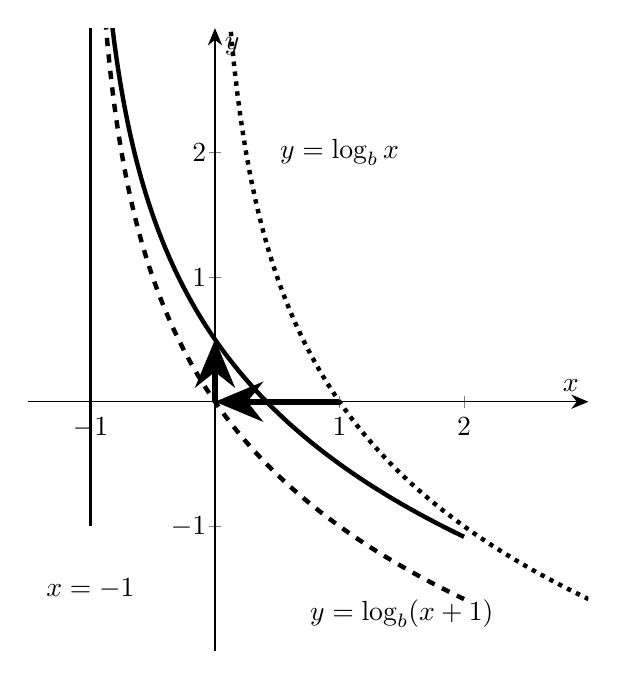
\begin{tikzpicture}[scale=1.0]
\pgfmathdeclarefunction{polyAAA}{0}{%
    \pgfmathparse{ln(x+1)/ln(0.5)+0.5}%
}
\pgfmathdeclarefunction{polyBBB}{0}{%
    \pgfmathparse{ln(x+1)/ln(0.5)}%
}

\pgfmathdeclarefunction{polyori}{0}{%
    \pgfmathparse{ln(x)/ln(0.5)}%
}
\begin{axis}[
unit vector ratio*=1 1 1,
axis lines = middle,
axis line style =  {-{Stealth[scale=1.3,angle'=45]}},
width=11cm,
xlabel={$x$},
ylabel={$y$},
domain=-2:14,
ymin=-2,
ymax=+3,
xmin=-1.5,
xmax=+3,
xtick={-1,0,1,2},
ytick={-1,0,1,2},
samples=160,
y tick label style={, xshift=0.25em}
]
\draw[thick] (axis cs:-1,-1) -- (axis cs:-1,3);
\draw[line width=2.3pt,-{Stealth[scale=1.3,angle'=45]}] (axis cs:1,0 ) -- (axis cs:0,0);
\draw[line width=2.3pt,-{Stealth[scale=1.3,angle'=45]}] (axis cs:0,0 ) -- (axis cs:0,0.5);

\addplot[black,ultra thick,dashed,mark=none,domain=-0.9:2] {polyBBB} ;
\addplot[black,ultra thick,mark=none, domain=-0.9:2] {polyAAA} ;

\addplot[black,ultra thick,dotted,mark=none, domain=-0.9:3] {polyori} ;

\node at (axis cs:-1, -1.5) {$x=-1$};
\node at (axis cs:1, 2) {$y=\log_b x$};
\node at (axis cs:1.5, -1.7) {$y=\log_b (x+1)$};
\end{axis}
\end{tikzpicture}    

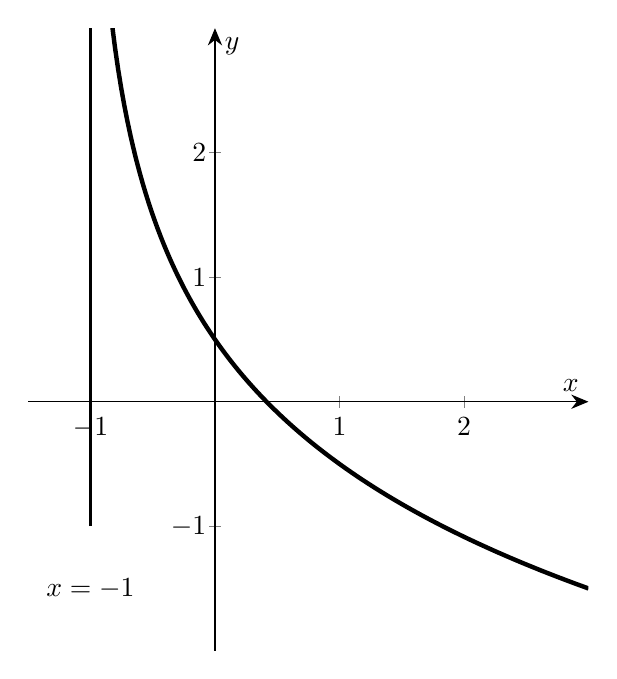
\begin{tikzpicture}[scale=1.0]
\pgfmathdeclarefunction{polyAAA}{0}{%
    \pgfmathparse{ln(x+1)/ln(0.5)+0.5}%
}
\begin{axis}[
unit vector ratio*=1 1 1,
axis lines = middle,
axis line style =  {-{Stealth[scale=1.3,angle'=45]}},
width=11cm,
xlabel={$x$},
ylabel={$y$},
domain=-2:14,
ymin=-2,
ymax=+3,
xmin=-1.5,
xmax=+3,
xtick={-1,0,1,2},
ytick={-1,0,1,2},
samples=160,
stack plots=y,
y tick label style={, xshift=0.25em}
]
\draw[thick] (axis cs:-1,-1) -- (axis cs:-1,3);

\addplot+[black,ultra thick,mark=none,stack plots=y, domain=-0.9:3] {polyAAA};
\node at (axis cs:-1, -1.5) {$x=-1$};

\end{axis}
\end{tikzpicture}

        \pgfmathdeclarefunction{polyB}{0}{%
    \pgfmathparse{ln(x+2)/ln(2)}%
}
\begin{tikzpicture}[scale=0.6]
\begin{axis}[
unit vector ratio*=1 1 1,
axis lines = middle,
axis line style =  {-{Stealth[scale=1.3,angle'=45]}},
width=11cm,
xlabel={$x$},
ylabel={$y$},
domain=-2:14,
ymin=-2,
ymax=10,
xmin=-2,
xmax=14,
xtick={-1,0,...,13},
ytick={-1,0,...,9},
samples=160,
stack plots=y
]
\newcommand{\nStartX}{1}
\newcommand{\nEndX}{8}
\draw[ultra thick] (axis cs:\nStartX,0) -- (axis cs:\nStartX,8);
\draw[ultra thick] (axis cs:\nEndX,0) -- (axis cs:\nEndX,8);
\draw[ultra thick] (axis cs:-5,0) -- (axis cs:12,0);

\addplot+[black,thick,mark=none,stack plots=y, domain=\nStartX:\nEndX] {polyB};
\addplot+[mark=none,fill=gray!20,draw=black,domain=\nStartX:\nEndX,stack plots=y] {min(0-(polyB),0)} \closedcycle;

\addplot+[black,thick,mark=none,stack plots=y, domain=-1.9:11] {polyB};
\node at (axis cs:12,4.5){ $\log_2 (x+2)$};
\node at (axis cs:\nStartX, 9) {$x=1$};
\node at (axis cs:\nEndX, 9) {$x=8$};
\node at (axis cs:6, -1.4) {圖一 $B$ 區域};
\end{axis}
\end{tikzpicture}
\pgfmathdeclarefunction{poly}{0}{%
    \pgfmathparse{ln(x)/ln(2)}%
}
\begin{tikzpicture}[scale=0.6]
\begin{axis}[
unit vector ratio*=1 1 1,
axis lines = middle,
axis line style =  {-{Stealth[scale=1.3,angle'=45]}},
width=11cm,
%xlabel={$x$},
%ylabel={$y$},
domain=-2:14,
ymin=-2,
ymax=10,
xmin=-2,
xmax=14,
xtick={-1,0,...,13},
ytick={-1,0,...,9},
samples=160,
stack plots=y
]
\newcommand{\nStartX}{3}
\newcommand{\nEndX}{10}


\draw[ultra thick] (axis cs:\nStartX,0) -- (axis cs:\nStartX,8);
\draw[ultra thick] (axis cs:\nEndX,0) -- (axis cs:\nEndX,8);

%畫 log 曲線與著色
\addplot+[black,thick,mark=none,stack plots=y, domain=\nStartX:\nEndX] {poly};
\addplot+[mark=none,fill=gray!20,draw=black,domain=\nStartX:\nEndX,stack plots=y] {min(0-(poly),0)} \closedcycle;
% 加強延伸 log f曲線部分
\addplot+[black,thick,mark=none,stack plots=y, domain=0.1:11] {poly};

\node at (axis cs:\nStartX, 9) {$x=3$};
\node at (axis cs:\nEndX, 9) {$x=10$};

\node at (axis cs:12,3.5){ $\log_2 x$};
\node at (axis cs:6, -1.4) {圖二};
\end{axis}
\end{tikzpicture}
\pgfmathdeclarefunction{polyA}{0}{%
    \pgfmathparse{ln(x)/ln(2)+5}%
}
\begin{tikzpicture}[scale=0.6]
\begin{axis}[
unit vector ratio*=1 1 1,
axis lines = middle,
axis line style = {-{Stealth[scale=1.3,angle'=45]}},
width=11cm,
%xlabel={$x$},
%ylabel={$y$},
domain=-2:14,
ymin=-2,
ymax=10,
xmin=-2,
xmax=14,
xtick={-1,0,...,13},
ytick={-1,0,...,9},
samples=160,
stack plots=y
]
\newcommand{\nStartX}{3}
\newcommand{\nEndX}{10}

\draw[ultra thick] (axis cs:\nStartX,0) -- (axis cs:\nStartX,8);
\draw[ultra thick] (axis cs:\nEndX,0) -- (axis cs:\nEndX,8.5);

\draw[ultra thick] (axis cs:0.5,5) -- (axis cs:12,5);

\draw [ pattern=north west lines, ultra thick] (axis cs:3,0) --(axis cs:3,5) -- (axis cs:10,5) -- (axis cs:10,0) -- (axis cs:3,0)  ;      


\addplot+[black,thick,mark=none,stack plots=y, domain=\nStartX:\nEndX] {polyA};
\addplot+[mark=none,fill=gray!20,draw=black,domain=\nStartX:\nEndX,stack plots=y] {min(0-(polyA),0)} \closedcycle;

\addplot+[black,thick,mark=none,stack plots=y, domain=0.1:11] {polyA};

\draw [ pattern=north west lines, ultra thick] (axis cs:3,0) --(axis cs:3,5) -- (axis cs:10,5) -- (axis cs:10,0) -- (axis cs:3,0)  ;

\node at (axis cs:12.3,8.5){ $\log_2 32x$};
\node at (axis cs:\nStartX, 9) {$x=3$};
\node at (axis cs:\nEndX, 9) {$x=10$};
\node at (axis cs:6, -1.4) {圖三 $A$ 區域};
\end{axis}
\end{tikzpicture}

    % !TEX encoding = UTF-8 Unicode
% !TEX TS-program = xelatex
\chapter{數列級數圖形}

\begin{tikzpicture}[scale=0.7]

\newcommand{\drawCutedPoint}[3]{
    
    \foreach \v in {0,1,...,#3}
    {
        \coordinate (cCutedPt) at ($ (#1) !{\v/#3}! (#2) $);
        \draw[ultra thick,fill] (cCutedPt) circle (1.5pt);
    }
    
}

\newcommand{\drawHexagon}[1]{
    \coordinate (cAPt) at (0: #1);
    \coordinate (cBPt) at (60:#1);
    \coordinate (cCPt) at (120:#1);
    \coordinate (cDPt) at (180:#1);
    \coordinate (cEPt) at (240:#1);
    \coordinate (cFPt) at (300:#1);
    
    \draw (cAPt)--(cBPt)--(cBPt)--(cCPt)--(cDPt)--(cEPt)--(cFPt) --cycle;
    
    \drawCutedPoint{cAPt}{cBPt}{#1};
    \drawCutedPoint{cBPt}{cCPt}{#1};
    \drawCutedPoint{cCPt}{cDPt}{#1};
    \drawCutedPoint{cDPt}{cEPt}{#1};
    \drawCutedPoint{cEPt}{cFPt}{#1};
    \drawCutedPoint{cFPt}{cAPt}{#1};
}

\begin{scope}[shift={(0,0)}]
\foreach \t in {1}
{
    \begin{scope}[shift={(120:\t)}]
    \drawHexagon{\t}
    \end{scope}
}
\node at (-0.5,-1){圖一};
\end{scope}
\begin{scope}[shift={(5,0)}]
\foreach \t in {1,2}
{
    \begin{scope}[shift={(120:\t)}]
    \drawHexagon{\t}
    \end{scope}
}
\node at (-1,-1){圖二};
\end{scope}
\begin{scope}[shift={(12,0)}]
\foreach \t in {1,2,...,3}
{
    \begin{scope}[shift={(120:\t)}]
    \drawHexagon{\t}
    \end{scope}
}
\node at (-1.5,-1){圖三};
\end{scope}
\end{tikzpicture}

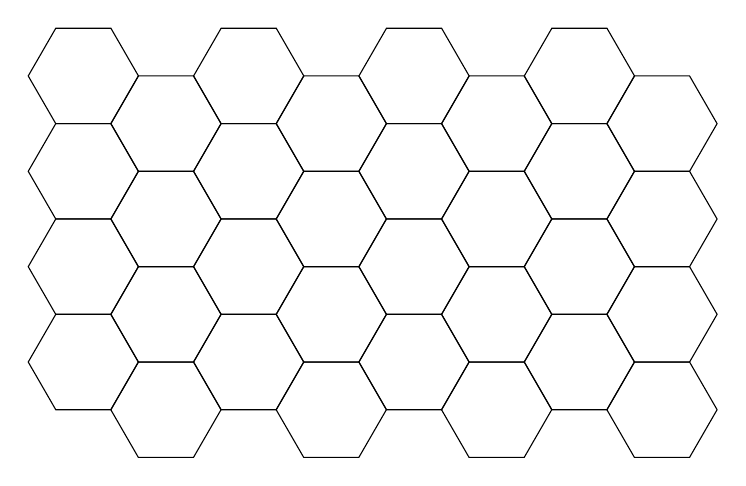
\begin{tikzpicture}[scale=0.7]

\foreach \beeCol in {0,1,2,3}
{
    \begin{scope} [shift = {(0:3 *\beeCol)} ]
    \begin{scope} [shift = {(0,0)}]
    \foreach \y in {0,1,2,3}
    {
        \begin{scope}[shift={(270:1.73* \y)}]
        %描述極坐標點
        \coordinate (cAPt) at (0: 1);
        \coordinate (cBPt) at (60:1);
        \coordinate (cCPt) at (120:1);
        \coordinate (cDPt) at (180:1);
        \coordinate (cEPt) at (240:1);
        \coordinate (cFPt) at (300:1);
        
        \draw (cAPt)--(cBPt)--(cBPt)--(cCPt)--(cDPt)--(cEPt)--(cFPt) --cycle;
        \end{scope}
    }
    \foreach \y in {0,1,2,3}
    {
        \begin{scope}[shift={(330:1.73)}]
        \begin{scope}[shift={(270:1.73* \y)}]
        %描述極坐標點
        \coordinate (cAPt) at (0: 1);
        \coordinate (cBPt) at (60:1);
        \coordinate (cCPt) at (120:1);
        \coordinate (cDPt) at (180:1);
        \coordinate (cEPt) at (240:1);
        \coordinate (cFPt) at (300:1);
        
        \draw (cAPt)--(cBPt)--(cBPt)--(cCPt)--(cDPt)--(cEPt)--(cFPt) --cycle;
        \end{scope}
        \end{scope}
        
    }
    
    \end{scope}
    \end{scope}
}
\end{tikzpicture}

        \begin{tikzpicture}
\newcommand\drawitemtwoone[1]
{        
    \begin{scope}[shift={(#1,0)}]
    {
        \filldraw[fill=lightgray,draw=black] (0,0) rectangle (2,1);
        \draw[dashed] (1,0) -- (1,1);
    }
    \end{scope}
}
\begin{scope}[shift={(0,0)}]


\foreach \x in {0,...,11}
{
    \begin{scope}[shift={(\x, 0)}]
    \filldraw[fill=white,draw=black] (0,0) rectangle (1,1);
    \end{scope}
}

\foreach \x in {1,3,6,8,10}
{
    \drawitemtwoone{\x};
}

\end{scope}
\node[below] at (6,0){圖一};
\end{tikzpicture}

\begin{tikzpicture}
\newcommand\drawitemtwoone[1]
{        
    \begin{scope}[shift={(#1,0)}]
    {
        \filldraw[fill=lightgray,draw=black] (0,0) rectangle (2,1);
        \draw[dashed] (1,0) -- (1,1);
    }
    \end{scope}
}
\begin{scope}[shift={(0,0)}]


\foreach \x in {0,...,11}
{
    \begin{scope}[shift={(\x, 0)}]
    \filldraw[fill=white,draw=black] (0,0) rectangle (1,1);
    \end{scope}
}

\foreach \x in {0,2,4,7,9}
{
    \drawitemtwoone{\x};
}

\end{scope}
\node[below] at (6,0){圖二};
\end{tikzpicture}

\begin{tikzpicture}
\newcommand\drawitemtwoone[1]
{        
    \begin{scope}[shift={(#1,0)}]
    {
        \filldraw[fill=lightgray,draw=black] (0,0) rectangle (2,1);
        \draw[dashed] (1,0) -- (1,1);
    }
    \end{scope}
}
\begin{scope}[shift={(0,0)}]


\foreach \x in {0,...,11}
{
    \begin{scope}[shift={(\x, 0)}]
    \filldraw[fill=white,draw=black] (0,0) rectangle (1,1);
    \end{scope}
}

\foreach \x in {1,4,6}
{
    \drawitemtwoone{\x};
}

\end{scope}
\node[below] at (6,0){圖三};
\end{tikzpicture}
\newpage
\begin{tikzpicture}
\begin{scope} 
\foreach \y in {0}
{
    \begin{scope}[shift={(330:1.73*2)}]
    \begin{scope}[shift={(270:1.73* \y)}]
    %描述極坐標點
    \coordinate (cAPt) at (0: 1);
    \coordinate (cBPt) at (60:1);
    \coordinate (cCPt) at (120:1);
    \coordinate (cDPt) at (180:1);
    \coordinate (cEPt) at (240:1);
    \coordinate (cFPt) at (300:1);
    
    \draw (cAPt)--(cBPt)--(cBPt)--(cCPt)--(cDPt)--(cEPt)--(cFPt) --cycle;
    \end{scope}
    \end{scope}
}

\end{scope}
\node[above] at (1,0) {圖一};
\node[above] at (5,0) {圖二};
\node[above] at (10,0) {圖三};

\begin{scope} [shift = {(5,0)}]
\foreach \y in {0,1}
{
    \begin{scope}[shift={(330:1.73)}]
    \begin{scope}[shift={(270:1.73* \y)}]
    %描述極坐標點
    \coordinate (cAPt) at (0: 1);
    \coordinate (cBPt) at (60:1);
    \coordinate (cCPt) at (120:1);
    \coordinate (cDPt) at (180:1);
    \coordinate (cEPt) at (240:1);
    \coordinate (cFPt) at (300:1);
    
    \draw (cAPt)--(cBPt)--(cBPt)--(cCPt)--(cDPt)--(cEPt)--(cFPt) --cycle;
    \end{scope}
    \end{scope}
    
}

\foreach \y in {0}
{
    \begin{scope}[shift={(330:1.73*2)}]
    \begin{scope}[shift={(270:1.73* \y)}]
    %描述極坐標點
    \coordinate (cAPt) at (0: 1);
    \coordinate (cBPt) at (60:1);
    \coordinate (cCPt) at (120:1);
    \coordinate (cDPt) at (180:1);
    \coordinate (cEPt) at (240:1);
    \coordinate (cFPt) at (300:1);
    
    \draw (cAPt)--(cBPt)--(cBPt)--(cCPt)--(cDPt)--(cEPt)--(cFPt) --cycle;
    \end{scope}
    \end{scope}
}
\end{scope}

\begin{scope} [shift = {(12,0)}]
\foreach \y in {0,1,2}
{
    \begin{scope}[shift={(270:1.73* \y)}]
    %描述極坐標點
    \coordinate (cAPt) at (0: 1);
    \coordinate (cBPt) at (60:1);
    \coordinate (cCPt) at (120:1);
    \coordinate (cDPt) at (180:1);
    \coordinate (cEPt) at (240:1);
    \coordinate (cFPt) at (300:1);
    
    \draw (cAPt)--(cBPt)--(cBPt)--(cCPt)--(cDPt)--(cEPt)--(cFPt) --cycle;
    \end{scope}
}
\foreach \y in {0,1}
{
    \begin{scope}[shift={(330:1.73)}]
    \begin{scope}[shift={(270:1.73* \y)}]
    %描述極坐標點
    \coordinate (cAPt) at (0: 1);
    \coordinate (cBPt) at (60:1);
    \coordinate (cCPt) at (120:1);
    \coordinate (cDPt) at (180:1);
    \coordinate (cEPt) at (240:1);
    \coordinate (cFPt) at (300:1);
    
    \draw (cAPt)--(cBPt)--(cBPt)--(cCPt)--(cDPt)--(cEPt)--(cFPt) --cycle;
    \end{scope}
    \end{scope}
    
}

\foreach \y in {0}
{
    \begin{scope}[shift={(330:1.73*2)}]
    \begin{scope}[shift={(270:1.73* \y)}]
    %描述極坐標點
    \coordinate (cAPt) at (0: 1);
    \coordinate (cBPt) at (60:1);
    \coordinate (cCPt) at (120:1);
    \coordinate (cDPt) at (180:1);
    \coordinate (cEPt) at (240:1);
    \coordinate (cFPt) at (300:1);
    
    \draw (cAPt)--(cBPt)--(cBPt)--(cCPt)--(cDPt)--(cEPt)--(cFPt) --cycle;
    \end{scope}
    \end{scope}
}
\end{scope}


\end{tikzpicture}


\newpage

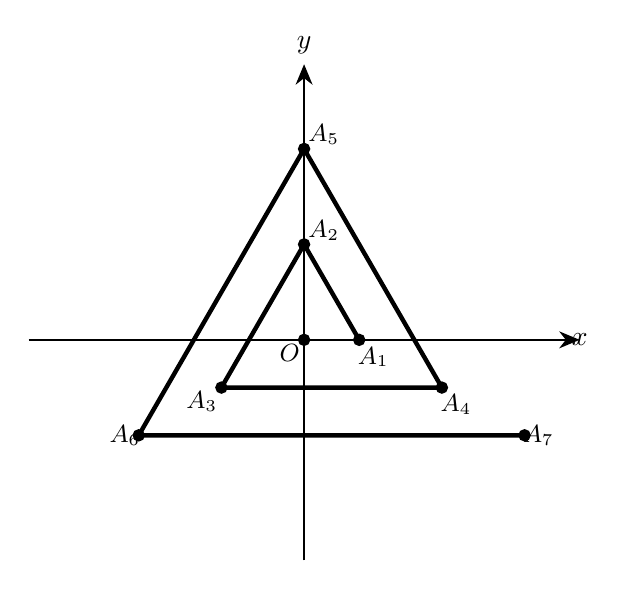
\begin{tikzpicture}[scale=0.7]
%x y axes
\draw[-{Stealth[scale=1.3,angle'=45]},semithick] (-5,0) -- (5,0) node[] {$x$};
\draw[-{Stealth[scale=1.3,angle'=45]},semithick] (0,-4)->(0,5)   node[above] {$y$};
%標示直角角度
\coordinate (cOPt) at (0,0);
\coordinate (cA1Pt) at (0:1);
\coordinate (cA2Pt) at ( $(120:2) + (cA1Pt)$ ) ;
\coordinate (cA3Pt) at ( $(240:3) + (cA2Pt)$ ) ;
\coordinate (cA4Pt) at ( $(0:4) + (cA3Pt)$ ) ;
\coordinate (cA5Pt) at ( $(120:5) + (cA4Pt)$ ) ;
\coordinate (cA6Pt) at ( $(240:6) + (cA5Pt)$ ) ;
\coordinate (cA7Pt) at ( $(0:7) + (cA6Pt)$ ) ;

\draw [ultra thick] (cA1Pt) -- (cA2Pt) -- (cA3Pt) --(cA4Pt) --(cA5Pt) --(cA6Pt) --(cA7Pt)  ;
\small
\foreach \v/\u/\t in 
{cOPt/225/$O$,
    cA1Pt/-10/$A_1$,
    cA2Pt/45/$A_2$,
    cA3Pt/225/$A_3$,
    cA4Pt/-10/$A_4$,
    cA5Pt/45/$A_5$,
    cA6Pt/180/$A_6$,
    cA7Pt/-1/$A_7$
}
{
    \draw[ultra thick,fill] (\v) circle (2pt);
    \node[label={[label distance=-0.25cm]\u:\t}] at (\v){};
    
};
\end{tikzpicture}

    \begin{tikzpicture}[scale=0.6]
%火柴棒排三角形
\coordinate (cOPt) at (0,0);
\coordinate (cAPt) at (0:2);
\coordinate (cBPt) at (60:2);
\draw[ultra thick] (cOPt) -- (cAPt) -- (cBPt) -- (cOPt) circle;

\foreach \v in {cOPt,cAPt,cBPt}
{
    \draw[ultra thick,fill] (\v) circle (3pt);
};

\node[label=270:圖1] at (1,0){};


\begin{scope}[shift={(5,0)}]
\coordinate (cOPt) at (0,0);
\coordinate (cAPt) at (0:2);
\coordinate (cA2Pt) at (0:4);
\coordinate (cBPt) at (60:2);
\coordinate (cB2Pt) at (60:4);
\coordinate (cMPt) at ($ (cA2Pt) !.5! (cB2Pt) $);
\draw[ultra thick] (cOPt) -- (cAPt) -- (cBPt) -- (cOPt) circle;
\draw[ultra thick] (cOPt) -- (cA2Pt) -- (cB2Pt) -- (cOPt) circle;
\draw[ultra thick] (cAPt) --  (cMPt) circle; 

\foreach \v in {cOPt,cAPt,cA2Pt,cBPt,cB2Pt,cMPt}
{
    \draw[ultra thick,fill] (\v) circle (3pt);
};
\node[label=270:圖2] at (2,0){};
\end{scope}

\begin{scope}[shift={(12,0)}]
\coordinate (cOPt) at (0,0);
\coordinate (cAPt) at (0:2);
\coordinate (cA2Pt) at (0:4);
\coordinate (cBPt) at (60:2);
\coordinate (cB2Pt) at (60:4);
\draw[ultra thick] (cOPt) -- (cAPt) -- (cBPt) -- (cOPt) circle;
\draw[ultra thick] (cOPt) -- (cA2Pt) -- (cB2Pt) -- (cOPt) circle;
\draw[ultra thick] (cAPt) -- ($ (cA2Pt) !.5! (cB2Pt) $) circle; 
\begin{scope}[shift={(6,0)}]
\coordinate (cA3Pt) at (0,0);
\coordinate (cCPt) at (-2,0);
\coordinate (cDPt) at (120:2);
\coordinate (cD2Pt) at (120:4);
\coordinate (cD3Pt) at (120:6);

\end{scope}

\draw[ultra thick] (cOPt) -- (cA3Pt) -- (cD3Pt)  -- (cOPt) ;
\coordinate (cMPt) at  ($ (cA2Pt) !.5! (cB2Pt) $);   %中點定位法
\draw[ultra thick] (cMPt) -- (cD2Pt) ;
\draw[ultra thick] (cA2Pt) -- (cDPt);

\foreach \v in {cOPt,cAPt,cA2Pt,cA3Pt,cBPt,cB2Pt,cMPt,cDPt,cD2Pt,cD3Pt}
{
    \draw[ultra thick,fill] (\v) circle (3pt);
};
\node[label=270:圖3] at (3,0){};
\end{scope}
\end{tikzpicture}
    % !TEX encoding = UTF-8 Unicode
% !TEX TS-program = xelatex

\chapter{排列組合相關圖形}
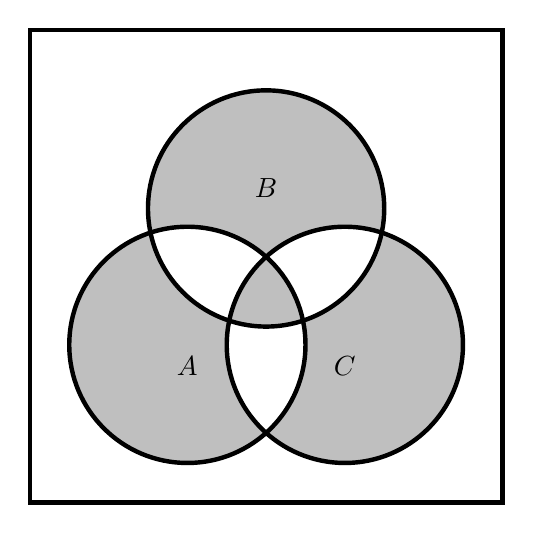
\begin{tikzpicture}
\def\firstcircle{(0,0) circle (1.5cm)}
\def\secondcircle{(60:2cm) circle (1.5cm)}
\def\thirdcircle{(0:2cm) circle (1.5cm)}

% Now we want to highlight the intersection of the first and the
% second circle:
\begin{scope}
\fill [lightgray] \firstcircle;
\end{scope}
\begin{scope}
\fill [lightgray] \secondcircle;
\end{scope}
\begin{scope}
\fill [lightgray] \thirdcircle;
\end{scope}


\begin{scope}
\clip \firstcircle;
\fill[white] \secondcircle;
\end{scope}
\begin{scope}
\clip \secondcircle;
\fill[white] \thirdcircle;
\end{scope}

\begin{scope}
\clip \thirdcircle;
\fill[white] \firstcircle;
\end{scope}

% Next, we want the highlight the intersection of all three circles:

\begin{scope}
\clip \firstcircle;
\clip \secondcircle;
\fill[lightgray] \thirdcircle;
\end{scope}

\draw [ultra thick] \firstcircle node[below] {$A$};
\draw [ultra thick] \secondcircle node [above] {$B$};
\draw [ultra thick] \thirdcircle node [below] {$C$};

\draw [ultra thick] (-2cm,-2cm) rectangle  (4cm,4cm);

\end{tikzpicture}

    \begin{tikzpicture}

\foreach \v in {0,1}
{
    \foreach \u in {0,1,2}
    {
        \draw[ultra thick] (\v,\u) -- (\v,{\u+1}) -- ({\v+1},{\u+1}) -- ({\v+1},{\u}) -- (\v,\u) circle;
    };
};
\coordinate (cAPt) at (0,0);
\coordinate (cBPt) at (2,3);
\coordinate (cCPt) at (1,2);
\coordinate (cDPt) at (1,3);
\coordinate (cEPt) at (2,2);

\foreach \v/\u/\t in 
{cAPt/180/$A$,
    cBPt/90/$B$,
    cDPt/90/$D$,
    cCPt/225/$C$,
    cEPt/0/$E$}
{
    \draw[ultra thick,fill] (\v) circle (2pt);
    \node[label=\u:\t] at (\v){};
    
};
\begin{scope}[shift={(3,2)}]
\draw[ultra thick,-latex] (0,0) -- (0,1) ;
\draw[ultra thick,-latex] (0,0) -- (1,0) ;
\node [label=0:東] at (1,0){};
\node [label=90:北] at (0,1){};

\end{scope}
\end{tikzpicture}

    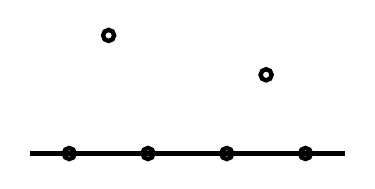
\begin{tikzpicture}

\draw [ultra thick](0.5,0) -- (4.5,0);

\draw[ultra thick] (1,0) circle (2pt);
\draw[ultra thick] (2,0) circle (2pt);
\draw[ultra thick] (3,0) circle (2pt);
\draw[ultra thick] (4,0) circle (2pt);
\draw[ultra thick] (1.5,1.5) circle (2pt);
\draw[ultra thick] (3.5,1) circle (2pt);
\end{tikzpicture}

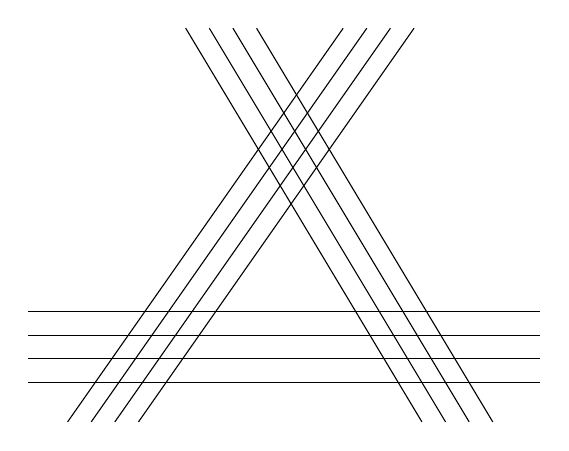
\begin{tikzpicture}[scale=1]
\newcommand{\HOfLine}{0.3};
\foreach \v in 
{0,...,3}
{
    \draw  ({-0.5  } , {0.5+\HOfLine*\v})  -- ({6}, {0.5+\HOfLine*\v});
}

\foreach \v in 
{0,...,3}
{
    \draw  ({0 +  \HOfLine*\v} , {0})  -- ({3.5+\HOfLine*\v}, {5});
}

\foreach \v in 
{0,...,3}
{
    \draw  ({4.5 +  \HOfLine*\v} , {0})  -- ({1.5+\HOfLine*\v}, {5});
}
\end{tikzpicture}

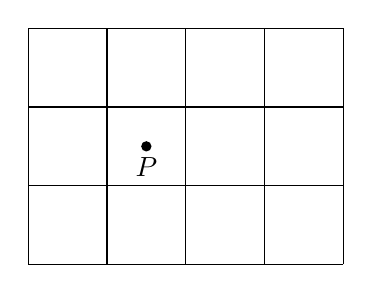
\begin{tikzpicture}[scale=1]

\coordinate (cPPt) at (1.5,1.5);
\draw[color=black] (0,0) grid (4,3);
\draw[ultra thick,fill] (cPPt) circle (1pt) node[ below ]  {$P$};

\end{tikzpicture}


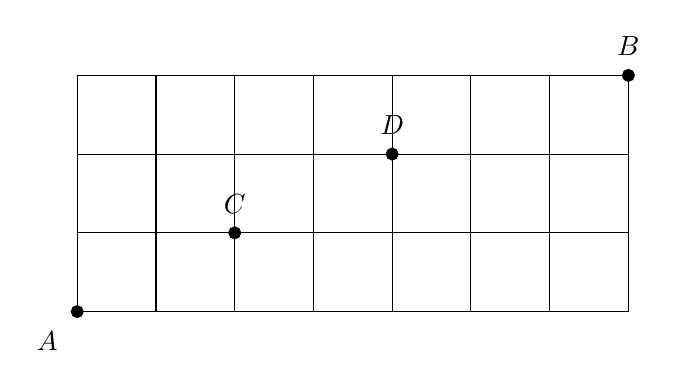
\begin{tikzpicture}[scale=1]

\coordinate (cAPt) at (0,0);
\coordinate (cBPt) at (7,3);
\coordinate (cCPt) at (2,1);
\coordinate (cDPt) at (4,2);
\draw[color=black] (0,0) grid (7,3);
%\draw[ultra thick,fill] (cPPt) circle (1pt) node[ below ]  {$P$};
\foreach \v/\u/\t in 
{   cAPt/225/$A$,
    cBPt/90 /$B$,
    cCPt/90 /$C$,
    cDPt/90 /$D$
}
{
    \draw[ultra thick,fill] (\v) circle (1.5pt);
    \node[label=\u:\t] at (\v){};
}; 

\end{tikzpicture}

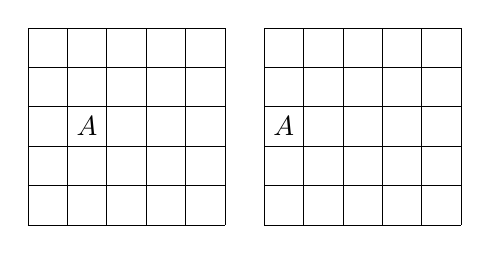
\begin{tikzpicture}[scale=.5]
\draw[very thin,color=black] (0,0) grid (5,5);

\def\seatSymbol{$\CIRCLE$}

\node at (1.5,2.5 ) {$A$};
\node at (1.5,3.5 ) {\seatSymbol};
\node at (1.5, 1.5) {\seatSymbol};
\node at (0.5,2.5) {\seatSymbol};
\node at (2.5, 2.5) {\seatSymbol};

\begin{scope}[shift={(6,0)}]
\draw[very thin,color=black] (0,0) grid (5,5);
\node at (0.5,2.5 ) {$A$};
\node at (0.5,3.5 ) {\seatSymbol};
\node at (0.5, 1.5) {\seatSymbol};
\node at (1.5, 2.5) {\seatSymbol};
\end{scope}
\end{tikzpicture}
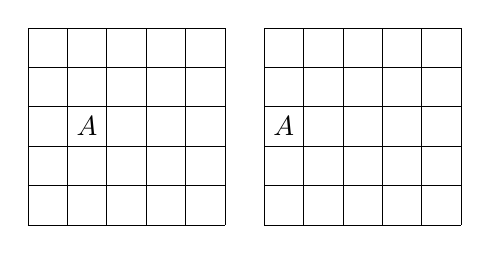
\begin{tikzpicture}[scale=.5]
\draw[very thin,color=black] (0,0) grid (5,5);

\def\seatSymbol{$\CIRCLE$}

\node at (1.5,2.5 ) {$A$};
\node at (1.5,3.5 ) {\seatSymbol};
\node at (1.5, 1.5) {\seatSymbol};
\node at (0.5,2.5) {\seatSymbol};
\node at (2.5, 2.5) {\seatSymbol};

\begin{scope}[shift={(6,0)}]
\draw[very thin,color=black] (0,0) grid (5,5);
\node at (0.5,2.5 ) {$A$};
\node at (0.5,3.5 ) {\seatSymbol};
\node at (0.5, 1.5) {\seatSymbol};
\node at (1.5, 2.5) {\seatSymbol};
\end{scope}
\end{tikzpicture}

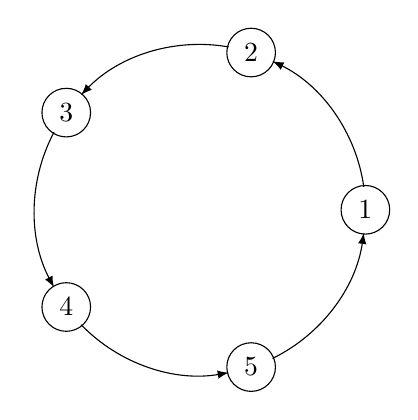
\begin{tikzpicture}[scale=0.7]

\def \n {5}
\def \radius {3cm}
\def \margin {8} % margin in angles, depends on the radius

\foreach \s in {1,...,\n}
{
    \node[draw, circle] at ({360/\n * (\s - 1)}:\radius) {$\s$};
    \draw[->, >=latex] ({360/\n * (\s - 1)+\margin}:\radius) 
    arc ({360/\n * (\s - 1)+\margin}:{360/\n * (\s)-\margin}:\radius);
}
\end{tikzpicture}


    \begin{tikzpicture}

\begin{scope}[shift={(0,0)}]
{
    \filldraw[fill=lightgray,draw=black] (0,0) rectangle (2,1);
    \draw[dashed] (1,0) -- (1,1);
    \node[above] at (0.5,1){積木};
}
\end{scope}
\begin{scope}[shift={(4,0)}]
\node[above] at (0.5,1){底板};
\foreach \x in {0,...,11}
{
    \begin{scope}[shift={(\x, 0)}]
    \filldraw[fill=white,draw=black] (0,0) rectangle (1,1);
    \end{scope}
}
\end{scope}

\end{tikzpicture}
    % !TEX encoding = UTF-8 Unicode
% !TEX TS-program = xelatex
\chapter{統計圖形}

\tikzset{
    treenode/.style = {shape=rectangle, rounded corners,
        draw, align=center,
        top color=white, bottom color=blue!20},
    root/.style     = {treenode, font=\Large, bottom color=red!30},
    env/.style      = {treenode, font=\ttfamily\normalsize},
    dummy/.style    = {circle,draw}
}
\begin{tikzpicture}
[
grow                    = right,
sibling distance        = 4em,
level distance          = 10em,
edge from parent/.style = {draw, -latex},
every node/.style       = {font=\footnotesize},
sloped
]
\node [root] {不孕症}
child { node [env] {第二類}
    child { node [env] {無法人工受孕}
        edge from parent node [below] {$1$} }
    edge from parent node [below] {$1-p$} }
child { node [env] {第一類}
    child { node [env] {人工受孕失敗}
        edge from parent node [below] {$1-q$} }
    child { node [env] {人工受孕成功}
        edge from parent node [above, align=center]
        {$q$}}
    edge from parent node [above] {$p$} };
\end{tikzpicture}

\tikzset{
    treenode/.style = {shape=rectangle, rounded corners,
        draw, align=center,
        top color=white, bottom color=blue!20},
    root/.style     = {treenode, font=\Large, bottom color=red!30},
    env/.style      = {treenode, font=\ttfamily\normalsize},
    dummy/.style    = {circle,draw}
}
\begin{tikzpicture}
[
grow                    = right,
%sibling distance        = 5em,
level 1/.style={sibling distance=20mm},
level 2/.style={sibling distance=10mm},
level distance          = 8em,
edge from parent/.style = {draw, -latex},
every node/.style       = {font=\footnotesize},
sloped
]
\node [root] {}
child { node [env] {丙袋}
    child { node [env] {兩球均白}
        edge from parent node [above] {$\frac{C^2_2}{C^5_2} = \frac{1}{10}$} }
    edge from parent node [below] {$\frac{1}{3}$} }
child { node [env] {乙袋}
    child { node [env] {兩球均白}
        edge from parent node [above] {$\frac{C^3_2}{C^{10}_2} = \frac{3}{45}$} }
    edge from parent node [below] {$\frac{1}{3}$} }
child { node [env] {甲袋}
    child { node [env] {兩球均白}
        edge from parent node [above] {$\frac{C^3_2}{C^6_2} = \frac{3}{15}$} }
    edge from parent node [below] {$\frac{1}{3}$} }
;
\end{tikzpicture}

\begin{tikzpicture}
[
grow                    = right,
%sibling distance        = 5em,
level 1/.style={sibling distance=20mm},
level 2/.style={sibling distance=10mm},
level distance          = 8em,
edge from parent/.style = {draw, -latex},
every node/.style       = {font=\footnotesize},
sloped
]
\node [root] {全班}
child { node [env] {沒談過}
    child { node [env] {$B$卷$=$畫 $\Circle$}
        edge from parent node [below] {$\frac{1}{4}$} }
    child { node [env] {$A$卷$=$畫 $\texttimes$} 
        edge from parent node [above, align=center]
        {$\frac{3}{4}$}}
    edge from parent node [below] {$40-p$} }
child { node [env] {有談過}
    child { node [env] {$B$卷$=$畫$ \texttimes$}
        edge from parent node [below] {$\frac{1}{4}$} }
    child { node [env] {$A$卷$=$畫 $\Circle$ }
        edge from parent node [above, align=center]
        {$\frac{3}{4}$}}
    edge from parent node [above] {$p$}
};

\end{tikzpicture}

\begin{tikzpicture}
[
grow                    = right,
%sibling distance        = 5em,
level 1/.style={sibling distance=20mm},
level 2/.style={sibling distance=10mm},
level distance          = 6em,
edge from parent/.style = {draw, -latex},
every node/.style       = {font=\footnotesize},
sloped
]
\node [root] {}
child { node [env] {真沒病}
    child { node [env] {檢驗沒病}
        edge from parent node [below] {$0.95$} }
    child { node [env] {檢驗有病} 
        edge from parent node [above, align=center]
        {$0.05$}}
    edge from parent node [below] {$0.8$} }
child { node [env] {真有病}
    child { node [env] {檢驗沒病}
        edge from parent node [below] {$0.1$} }
    child { node [env] {檢驗有病 }
        edge from parent node [above, align=center]
        {$0.9$}}
    edge from parent node [above] {$0.2$}
};

\end{tikzpicture}


\begin{tikzpicture}[line cap=round,line join=round,x=0.25cm,y=0.25cm]
\newcommand{\drawCutedPoint}[3]{
    \foreach \v in {1,2,...,#3}
    {
        \coordinate (cCutedPt) at ($ (#1) !{\v/#3}! (#2) $);
        \draw[ultra thick,fill] (cCutedPt) circle (1.5pt);
    }
}

\coordinate (cAPt) at (0,1);
\coordinate (cBPt) at (4,7);
\drawCutedPoint{cAPt}{cBPt}{4};
\draw[-{Stealth[scale=1,angle'=45]},color=black] (0,0.) -- (10,0.)  node[] {$x$};
\draw[-{Stealth[scale=1,angle'=45]},color=black] (0.,0) -- (0.,10) node[above] {$y$};
\end{tikzpicture}
\begin{tikzpicture}[line cap=round,line join=round,x=0.25cm,y=0.25cm]
\newcommand{\drawCutedPoint}[3]{
    \foreach \v in {1,2,...,#3}
    {
        \coordinate (cCutedPt) at ($ (#1) !{\v/#3}! (#2) $);
        \draw[ultra thick,fill] (cCutedPt) circle (1.5pt);
    }
}

\coordinate (cAPt) at (1,0);
\coordinate (cBPt) at (7,4);
\drawCutedPoint{cAPt}{cBPt}{4};
\draw[-{Stealth[scale=1,angle'=45]},color=black] (0,0.) -- (10,0.)  node[] {$x$};
\draw[-{Stealth[scale=1,angle'=45]},color=black] (0.,0) -- (0.,10) node[above] {$y$};
\end{tikzpicture}
\begin{tikzpicture}[line cap=round,line join=round,x=0.25cm,y=0.25cm]
\newcommand{\drawCutedPoint}[3]{
    \foreach \v in {1,2,...,#3}
    {
        \coordinate (cCutedPt) at ($ (#1) !{\v/#3}! (#2) $);
        \draw[ultra thick,fill] (cCutedPt) circle (1.5pt);
    }
}

\coordinate (cAPt) at (0,5);
\coordinate (cBPt) at (7,1);
\drawCutedPoint{cAPt}{cBPt}{4};
\draw[-{Stealth[scale=1,angle'=45]},color=black] (0,0.) -- (10,0.)  node[] {$x$};
\draw[-{Stealth[scale=1,angle'=45]},color=black] (0.,0) -- (0.,10) node[above] {$y$};
\end{tikzpicture}
\begin{tikzpicture}[line cap=round,line join=round,x=0.25cm,y=0.25cm]
\newcommand{\drawCutedPoint}[3]{
    \foreach \v in {1,2,...,#3}
    {
        \coordinate (cCutedPt) at ($ (#1) !{\v/#3}! (#2) $);
        \draw[ultra thick,fill] (cCutedPt) circle (1.5pt);
    }
}

\coordinate (cAPt) at (0,7);
\coordinate (cBPt) at (7,7);
\drawCutedPoint{cAPt}{cBPt}{4};
\draw[-{Stealth[scale=1,angle'=45]},color=black] (0,0.) -- (10,0.)  node[] {$x$};
\draw[-{Stealth[scale=1,angle'=45]},color=black] (0.,0) -- (0.,10) node[above] {$y$};
\end{tikzpicture}
\begin{tikzpicture}[line cap=round,line join=round,x=0.25cm,y=0.25cm]
\newcommand{\drawCutedPoint}[3]{
    \foreach \v in {1,2,...,#3}
    {
        \coordinate (cCutedPt) at ($ (#1) !{\v/#3}! (#2) $);
        \draw[ultra thick,fill] (cCutedPt) circle (1.5pt);
    }
}

\coordinate (cAPt) at (7,0);
\coordinate (cBPt) at (7,7);
\drawCutedPoint{cAPt}{cBPt}{4};
\draw[-{Stealth[scale=1,angle'=45]},color=black] (0,0.) -- (10,0.)  node[] {$x$};
\draw[-{Stealth[scale=1,angle'=45]},color=black] (0.,0) -- (0.,10) node[above] {$y$};
\end{tikzpicture}

\section{二項分布}
\begin{tikzpicture}[scale=0.85,
remember picture,
declare function={binom(\k,\n,\p)=\n!/(\k!*(\n-\k)!)*\p^\k*(1-\p)^(\n-\k);},
xshift=0cm,yshift=0cm
]
\begin{axis}[
xmin=0,ymin=0,
scale only axis,samples=2000,
samples at={0,...,10},
yticklabel style={
    /pgf/number format/fixed,
    /pgf/number format/fixed zerofill,
    /pgf/number format/precision=2
},
ybar=0pt, bar width=10
]
\addplot [fill=cyan, fill opacity=0.5] {binom(x,10,0.5)};
\addlegendentry{$p=0.5$}
\addplot[smooth, domain=0:10] {1/(sqrt(10/4)*sqrt(2*pi))*exp(-(\x-5)^2/(2*(sqrt(10/4))^2))};
\addlegendentry{Normal Dist.}

\end{axis}
\end{tikzpicture}
    % !TEX encoding = UTF-8 Unicode
% !TEX TS-program = xelatex

\chapter{三角}
\begin{tikzpicture}

\coordinate (cAPt) at (0,0);
\coordinate (cBPt) at (53:5);
\coordinate (cCPt) at (80.5:{2*sqrt(5)});
\coordinate (cDPt) at (3,0);


\foreach \v/\u/\t in 
{cAPt/180/$A$,
    cBPt/45/$B$,
    cCPt/135/$C$,
    cDPt/0/$D$
}
{
    \draw[ultra thick,fill] (\v) circle (2pt);
    \node[label=\u:\t] at (\v){};
};	    

\draw[ultra thick] (cAPt) -- (cDPt) -- (cBPt)  -- (cCPt) -- (cAPt) circle;
\draw[ultra thick] (cAPt) -- (cBPt) ;

\end{tikzpicture}

\begin{tikzpicture} %方格範例

\foreach \v in {0,1,2,3} % x方向
{
    \foreach \u in {0,1}
    {
        \draw[ultra thick] (\v,\u) -- (\v,{\u+1}) -- ({\v+1},{\u+1}) -- ({\v+1},{\u}) -- (\v,\u) circle;
    };
};


\begin{scope}[shift={(4,0)}]

\foreach \v in {0} % x方向
{
    \foreach \u in {0,2,4}
    {
        \draw[ultra thick] (\v,\u) -- (\v,{\u+2}) -- ({\v+2},{\u+2}) -- ({\v+2},{\u}) -- (\v,\u) circle;
    };
};
\end{scope}
\coordinate (cAPt) at (0,1);
\coordinate (cBPt) at (4,0);
\coordinate (cCPt) at (6,6);

\foreach \v/\u/\t in 
{cAPt/180/$A$,
    cBPt/270/$B$,
    cCPt/0/$C$}
{
    \draw[ultra thick,fill] (\v) circle (2pt);
    \node[label=\u:\t] at (\v){};
};	    
\end{tikzpicture}
\begin{tikzpicture}

\foreach \v in {0,1,2,3} % x方向
{
    \foreach \u in {0,1}
    {
        \draw[ultra thick] (\v,\u) -- (\v,{\u+1}) -- ({\v+1},{\u+1}) -- ({\v+1},{\u}) -- (\v,\u) circle;
    };
};


\begin{scope}[shift={(4,0)}]

\foreach \v in {0} % x方向
{
    \foreach \u in {0,2,4}
    {
        \draw[ultra thick] (\v,\u) -- (\v,{\u+2}) -- ({\v+2},{\u+2}) -- ({\v+2},{\u}) -- (\v,\u) circle;
    };
};
\end{scope}
\coordinate (cAPt) at (0,1);
\coordinate (cBPt) at (4,0);
\coordinate (cCPt) at (6,6);
\coordinate (cDPt) at (0,0);
\coordinate (cEPt) at (4,6);

\foreach \v/\u/\t in 
{cAPt/180/$A$,
    cBPt/270/$B$,
    cCPt/0/$C$,
    cDPt/180/$D$,
    cEPt/180/$E$
}
{
    \draw[ultra thick,fill] (\v) circle (2pt);
    \node[label=\u:\t] at (\v){};
};	    
\draw[ultra thick] (cAPt) -- (cBPt) -- (cCPt) circle;

\end{tikzpicture}

    \begin{tikzpicture}[scale=1.0]
%塔高立體圖
\coordinate (cxleftPt) at (-2,0);
\coordinate (cxPt) at (4,0);
\coordinate (cOPt) at (0,0);
\coordinate (cAPt) at (3,0);
\coordinate (cBPt) at (-45:3);
\coordinate (cTPt) at (0,3);
\coordinate (chalfTPt) at (0,1.5);

\coordinate (cyupPt) at (60:3);
\coordinate (cydownPt) at (240:3); 

\draw[-{Stealth[scale=1.3,angle'=45]},semithick] (cxleftPt) -- (cxPt) node[] {$x$};

\draw[-{Stealth[scale=1.3,angle'=45]},semithick] (cydownPt)->(cyupPt)   node[above] {$y$};
\draw[ultra thick] (cOPt) -- (cTPt);
\draw[ultra thick] (cOPt) -- (cBPt);
\draw[ultra thick] (cBPt) -- (cTPt);
\draw[ultra thick] (cOPt) -- (cAPt);
\draw[ultra thick] (cTPt) -- (cAPt);
\draw[ultra thick] (cAPt) -- (cBPt);


\draw[ultra thick] (cAPt) circle (1pt);
\draw[ultra thick] (cBPt) circle (1pt);
\draw[ultra thick] (cTPt) circle (1pt);

\node[label=225:$O$] at (cOPt){};
\node[label=10:$A$] at (cAPt){};
\node[label=175:$45^\circ$] at (cAPt){};
\node[label=0:$B$] at (cBPt){};
\node[label=355:$30^\circ$] at (-45:1){};
\node[label=180:$h$] at (chalfTPt){};
\node[label=272:$60^\circ$] at (cOPt){};


\end{tikzpicture}
    \begin{tikzpicture}[scale=1.5]
\coordinate (cOPt) at (0:0);
\coordinate (cAPt) at (0:1);
\coordinate (cBPt) at (56:1);	%粗略B值
\coordinate (cCPt) at (112:1);	%粗略C值

\draw[ultra thick] (cAPt) circle (1pt);
\draw[ultra thick] (cBPt) circle (1pt);
\draw[ultra thick] (cCPt) circle (1pt);


\draw[ultra thick] (0,0) circle (1);

\draw[ultra thick] (cOPt) -- (cCPt);
\node[label=225:$O$] at (cOPt){};
\node[label=10:$A$] at (cAPt){};

\node[label=56:$B$] at (cBPt){};
\node[label=112:$C$] at (cCPt){};
% x軸 y 軸 axes
\draw[-{Stealth[scale=1.3,angle'=45]},semithick] (-2,0) -- (2,0) node[] {$x$};
\draw[-{Stealth[scale=1.3,angle'=45]},semithick] (0,-2)->(0,2)   node[above] {$y$};

\end{tikzpicture}
\newline
\begin{tikzpicture}[scale=1.5]
\coordinate (cOPt) at (0:0);
\coordinate (cBPt) at (53:1);
\coordinate (cPPt) at (0:1);
\coordinate (yaxis) at (0,1);
\coordinate (xaxis) at (1,0);
\coordinate (cQPt) at (1, {4/3});
\coordinate (cCPt) at (0,{4/5});
\coordinate (cAPt) at ({3/5},0);
\draw[ultra thick] (yaxis |- cBPt) node[left] {$C$} -| (xaxis -| cBPt) node[below] {$A$};

%\draw[ultra thick] (cBPt) circle (3pt);

\draw[ultra thick] (0,0) circle (1);
\draw [ultra thick] (cQPt) -- (cPPt);
\draw [ultra thick] (cQPt) -- (cOPt);

\node[label=90:$B$] at (cBPt){};
\node[label=225:$O$] at (cOPt){};
\node[label={[label distance=0.0cm]5:$P$}] at (cPPt){};
\node[label=45:$Q$] at (cQPt){};

%標示直角角度
\newcommand{\nRect}{0.2cm}
\def\rectanglepath{-- +(-\nRect,0cm) -- +(-\nRect,+\nRect) -- +(0cm,\nRect) -- cycle} 
\draw (cAPt) \rectanglepath;
\newcommand{\nRectR}{-0.2cm}
\def\rectanglepathFour{-- +(-\nRectR,0cm) -- +(-\nRectR,+\nRectR) -- +(0cm,\nRectR) -- cycle} 
\draw (cAPt) \rectanglepath;
\draw (cCPt) \rectanglepathFour;

% x軸 y 軸 axes
\draw[-{Stealth[scale=1.3,angle'=45]},semithick] (-2,0) -- (2,0) node[] {$x$};
\draw[-{Stealth[scale=1.3,angle'=45]},semithick] (0,-2)->(0,2)   node[above] {$y$};

\end{tikzpicture}
\newpage
\begin{tikzpicture}[scale=1.0]
%利用坐標給定位置
\coordinate (cAPt) at (0,3);
\coordinate (cBPt) at (6,3);
\coordinate (cCPt) at (6,0);
\coordinate (cDPt) at (0,0);
\coordinate (cEPt) at (2,0);
\coordinate (cFPt) at (0.7,0.2);

%畫出封閉型區域
\draw [ultra thick](cAPt)--(cBPt)--(cCPt)--(cDPt)--(cAPt) circle;

\draw [ultra thick] (cAPt) -- (cCPt);
\draw [ultra thick] (cEPt) -- (cBPt);

%計算出交點座標
\coordinate (cPPt) at (intersection of cAPt--cCPt and cEPt--cBPt);

\draw [ultra thick] (cFPt) -- (cAPt);
\draw [ultra thick] (cFPt) -- (cPPt);

\node[label=135:$A$] at (cAPt){};
\node[label=45:$B$] at (cBPt){};
\node[label=-45:$C$] at (cCPt){};
\node[label=225:$D$] at (cDPt){};
\node[label=225:$E$] at (cEPt){};
\node[label=90:$P$] at (cPPt){};
\node[label=$\theta$] at (2.6,0.2){};
\node[label=45:$F$] at (cFPt){};

% x軸 y 軸 axes
%    \draw[-{Stealth[scale=1.3,angle'=45]},semithick] (-6,0) -- (6,0) node[] {$x$};
%    \draw[-{Stealth[scale=1.3,angle'=45]},semithick] (0,-6)->(0,6)   node[above] {$y$};
\end{tikzpicture}
    \begin{tikzpicture}[scale=0.6]
\newcommand{\nSide}{5}
\newcommand{\nLittleSide}{\nSide *0.5176}


%\coordinate (cAPt) at ({\nSide/2},{\nSide * sqrt(3) /2 });
%\coordinate (cBPt) at (0, 0);
%\coordinate (cCPt) at (\nSide, 0);
%\coordinate (cFPt) at (15:{\nLittleSide});
%\coordinate (cEPt) at (15:{\nDiffSide});
%\coordinate (cDPt) at (15:{\nDiffSide} + 60:\nDiffSide);

\coordinate (cAPt) at (90:\nSide);
\coordinate (cBPt) at (210:\nSide);
\coordinate (cCPt) at (330:\nSide);
\coordinate (cDPt) at (105:\nLittleSide);
\coordinate (cEPt) at (225:\nLittleSide);
\coordinate (cFPt) at (345:\nLittleSide);

\filldraw[fill=green!20,draw=green!50!black] (cBPt) -- ++ (0:2) arc (0:15:2) -- cycle;
\filldraw[fill=green!20,draw=green!50!black] (cAPt) -- ++ (240:2) arc (240:255:2) -- cycle;
\filldraw[fill=green!20,draw=green!50!black] (cCPt) -- ++(120:2) arc (120:135:2) -- cycle;

\coordinate (cAngle1) at ($(cBPt)!0.2!8:(cCPt)$);
\node[label=0:$1$] at (cAngle1){};
\coordinate (cAngle2) at ($(cCPt)!0.2!8:(cAPt)$);
\node[label=120:$2$] at (cAngle2){};
\coordinate (cAngle3) at ($(cAPt)!0.2!8:(cBPt)$);
\node[label=266:$3$] at (cAngle3){};



\draw [ultra thick](cAPt)--(cBPt);
\draw [ultra thick](cAPt)--(cCPt);
\draw [ultra thick](cBPt)--(cCPt);
\draw [ultra thick](cBPt)--(cFPt);
\draw [ultra thick](cAPt)--(cEPt);
\draw [ultra thick](cCPt)-- (cDPt);

%\draw [ultra thick](cCPt)--(cDPt);


%\draw [ultra thick] (10,0) arc [radius=5, start angle=0, end angle= 180];

\node[label=90:$A$] at (cAPt){};
\node[label=180:$B$] at (cBPt){};
\node[label=0:$C$] at (cCPt){};
\node[label=75:$D$] at (cDPt){};
\node[label=165:$E$] at (cEPt){};
\node[label=270:$F$] at (cFPt){};
\node[label=270:$F$] at (cFPt){};

\end{tikzpicture}
\begin{tikzpicture}[scale=0.6, font=\large]
\newcommand{\nSide}{5}
\newcommand{\nAngle}{360 /5}



\coordinate (cAPt) at ({\nAngle*1-90}:\nSide);
\coordinate (cBPt) at ({\nAngle*2-90}:\nSide);
\coordinate (cCPt) at ({\nAngle*3-90}:\nSide);
\coordinate (cDPt) at ({\nAngle*4-90}:\nSide);
\coordinate (cEPt) at (-90:\nSide)           ;

\draw [ultra thick](cAPt)--(cBPt)--(cCPt)--(cDPt)--(cEPt)--(cAPt) circle;
\node[label=\nAngle*1-90:$A$] at (cAPt){};
\node[label=\nAngle*2-90:$B$] at (cBPt){};
\node[label=\nAngle*3-90:$C$] at (cCPt){};
\node[label=\nAngle*4-90:$D$] at (cDPt){};
\node[label=\nAngle*5-100:$E$] at (cEPt){};
%x y axes
\draw[-{Stealth[scale=1.3,angle'=45]},semithick] (-6,0) -- (6,0) node[] {$x$};
\draw[-{Stealth[scale=1.3,angle'=45]},semithick] (0,-6)->(0,6)   node[above] {$y$};

\end{tikzpicture}
    \begin{tikzpicture}[scale=1, font=\large]
\coordinate (cCPt) at (0,0);
\coordinate (cBPt) at (0,3);
\coordinate (cAPt) at (4,0);
\draw [ultra thick](cAPt)--(cBPt)--(cCPt)--cycle;
%利用旋轉做出圖形 cBPt 為圓心 1 倍線段長(cAPt)度為半徑,逆時針旋轉90度
\coordinate (cDPt) at ($(cBPt)!1!90:(cAPt)$);
\coordinate (cEPt) at ($(cAPt)!1!-90:(cBPt)$);

\draw [ultra thick] (cAPt) -- (cBPt) -- (cDPt) -- (cEPt) -- cycle;

\node[label=315:$A$] at (cAPt){};
\node[label=180:$B$] at (cBPt){};
\node[label=225:$C$] at (cCPt){};
\node[label=45:$D$] at (cDPt){};
\node[label=30:$E$] at (cEPt){};

\end{tikzpicture}

\begin{tikzpicture}[scale=0.5, font=\large]
\newcommand{\nCx}{{3*sqrt(19)}}
\newcommand{\nBx}{{-sqrt(19)}}
\newcommand{\nAy}{{12*sqrt(3/19)}}
\newcommand{\nAx}{{sqrt(27-(144*3/19))}}

\coordinate (cDPt) at (0,0);
\coordinate (cCPt) at (\nCx, 0);
\coordinate (cBPt) at (\nBx,0);
\coordinate (cAPt) at (\nAx,\nAy);
\draw [ultra thick](cAPt)--(cBPt)--(cCPt)--cycle;

\draw [ultra thick] (cAPt) -- (cDPt);

\node[label=90:$A$] at (cAPt){};
\node[label=180:$B$] at (cBPt){};
\node[label=0:$C$] at (cCPt){};
\node[label=270:$D$] at (cDPt){};

%漂亮標示角度
\pic [draw, -, "$30^\circ$", angle eccentricity=2.3] {angle = cBPt--cAPt--cDPt};
%標示直角角度
\coordinate (O) at (cCPt);
\coordinate (A) at (cAPt);
\path (A) -- ($(A)!1cm!(O)$)coordinate (A1);
\path (A) -- ($(A)!1cm!(cDPt)$)coordinate (A3);
\path (A) -- ($(A3)!1cm!-90:(A)$)coordinate (A2);
\draw (A)--(A1) -- (A2) --(A3)--cycle;

\end{tikzpicture}

\begin{tikzpicture}[scale=1, font=\large]
\newcommand{\nSide}{5}
\newcommand{\nAngle}{360 /5}



\coordinate (cBPt) at (0,0);
\coordinate (cAPt) at (0:\nSide);
\coordinate (cCPt) at (45:{sqrt(2)* \nSide});
\coordinate (cMPt) at ($(cAPt)!0.5!(cCPt)$);
\draw [ultra thick](cAPt)--(cBPt)--(cCPt)--cycle;
\draw [ultra thick] (cBPt) -- (cMPt);

\node[label=315:$A$] at (cAPt){};
\node[label=225:$B$] at (cBPt){};
\node[label=80:$C$] at (cCPt){};
\node[label=0:$M$] at (cMPt){};
%漂亮標示角度
\pic [draw, -, "$\theta$", angle eccentricity=2.5] {angle = cMPt--cBPt--cCPt};
\newcommand{\nRect}{0.5cm}
%標示直角角度
\def\rectanglepath{-- +(-\nRect,0cm) -- +(-\nRect,+\nRect) -- +(0cm,\nRect) -- cycle}
\draw (cAPt) \rectanglepath;
\end{tikzpicture}


    \begin{tikzpicture}[scale=.5] % 已知三邊長畫出 三角形ABC


\def\sAB{5}
\def\sAC{6}
\def\sBC{8}

\coordinate [label=below:$B$] (B) at (0,0);
\coordinate [label=below:$C$] (C) at (\sBC,0);
\begin{pgfinterruptboundingbox}
\node (Circ1) at (C) [circle through=($ (C) + (0:\sAC) $)] {};
\node (Circ2) at (B) [circle through=($ (B) + (0:\sAB) $)] {};
\end{pgfinterruptboundingbox}
\coordinate [label=above:$A$] (A) at (intersection 2 of Circ2 and Circ1);
\draw (A) -- (B) -- (C) -- cycle;
\tkzLabelSegment[midway,  below](B,C){$\sBC$ };
\tkzLabelSegment[midway,  above ](A,C){$\sAC$};
\tkzLabelSegment[midway,  above left](A,B){$\sAB$};
\end{tikzpicture}

\begin{tikzpicture}[scale = 0.4]
\draw (0.,0.)-- (7.,0.);
\draw (7.,0.)-- (0.824,5.098);
\draw (0.824,5.098)-- (0.,0.);
\draw (0.824,5.098)-- (7.,0.);
\draw (7.,0.)-- (12.098,6.175);
\draw (12.098,6.175)-- (5.923,11.274333612170306);
\draw (5.923,11.274333612170306)-- (0.824,5.098);
\draw (0.,0.)-- (0.824,5.098);
\draw (0.824,5.098)-- (-4.274333612170306,5.923089457836511);
\draw (-4.274333612170306,5.923089457836511)-- (-5.098,0.8243779228331025);
\draw (-5.098,0.8243779228331025)-- (0.,0.);
\draw [fill=black] (0.,0.) circle (1.5pt);
\draw[color=black] (-0.5032213038841461,-0.7427250625524924) node {$B$};
\draw [fill=black] (7.,0.) circle (2.5pt);
\draw[color=black] (8.590833399129002,0.584874164164758) node {$C$};
\draw [fill=black] (0.824,5.098) circle (2.5pt);
\draw[color=black] (0.824,6.95735045240756) node {$A$};
\draw [fill=black] (12.098,6.175) circle (2.5pt);
\draw[color=black] (12.97191084729592,7.355630220422735) node {$F$};
\draw [fill=black] (5.923,11.274333612170306) circle (2.5pt);
\draw[color=black] (6.798574443060717,12.466887243284148) node {$G$};
\draw [fill=black] (-4.274333612170306,5.923089457836511) circle (1.5pt);
\draw[color=black] (-4.154119177356578,7.6211500657661855) node {$E$};
\draw [fill=black] (-5.098,0.8243779228331025) circle (1.5pt);
\draw[color=black] (-6.477417824111762,1.0495338935157956) node {$D$};
\end{tikzpicture}

    \begin{tikzpicture}
\coordinate (cAPt) at (-3.91, 0.85);
\coordinate (cBPt) at (-0.83, -3.91); 
\coordinate (cCPt) at (2.4, 3.2);
\coordinate (cDPt) at (-1.57, 3.68);
\coordinate (cOPt) at (0, 0);

\draw (cAPt) -- (cBPt) -- (cCPt) -- (cDPt) -- cycle;
\draw (cAPt) -- (cCPt);
\draw (cOPt) circle (4);


\tkzMarkAngle(cCPt,cAPt,cDPt);
\tkzLabelAngle[pos=1.5](cDPt,cAPt,cCPt){$30^\circ$};

\tkzMarkAngle(cAPt,cCPt,cBPt);
\tkzLabelAngle[pos=1.5](cAPt,cCPt,cBPt){$45^\circ$};

\foreach \v/\u/\t in 
{   cAPt/225/$A$,
    cBPt/270/$B$,
    cCPt/45/$C$,
    cDPt/90/$D$
}
{
    \draw[ultra thick,fill] (\v) circle (0.8pt);
    \node[label=\u:\t] at (\v){};
};
\end{tikzpicture}

        \begin{tikzpicture}[scale=1.3]
\coordinate (cOPt) at (0,0);
\draw[-{Stealth[scale=1,angle'=45]},color=black] (-2,0.) -- (2,0.)  node[] {$x$};
%\foreach \x in {-3,-2,-1,1,2}
%\draw[shift={(\x,0)},color=black] (0pt,2pt) -- (0pt,-2pt) node[below] {\footnotesize $\x$};
\draw[-{Stealth[scale=1,angle'=45]},color=black] (0.,-2.) -- (0.,2) node[above] {$y$};
\draw (cOPt) circle (1);
\foreach \v in 
{
    1,2,3,4,5
}
{
    \draw[ultra thick,fill] (\v * 57.3: 1) circle (0.8pt);
    %\node[above] at (\v,0){$\v$};
}

\foreach \v/\u/\t in 
{   1/57/$1$,
    2/114/$2$,
    3/171/$3$,
    4/228/$4$,
    5/285/$5$
}
{
    \draw [-{Stealth[scale=1.3,angle'=45]},semithick] (cOPt) -- (\v * 57.3:1.5) ;
    \node[label=\u:\t] at (\v * 57.3:1.5){};
};
\end{tikzpicture}

\section{極坐標}
         \begin{tikzpicture}[scale=2]
\draw[->] (-1,0) -- (1,0);
\draw[->] (0,-1) -- (0,1);
\draw node [red] at (-1,.25) {\scriptsize{Kardioida $r=1+\sin
        \theta$}};
\draw[color=red,domain=0:6.28,samples=200,smooth] plot (canvas polar
cs:angle=\x r,radius=      {5+5*sin(\x r)});    %r = angle en radian
\end{tikzpicture}

\begin{tikzpicture}[scale=2]
\draw[->] (-1,0) -- (1,0);
\draw[->] (0,-1) -- (0,1);
\draw node [red] at (-1,.25) {\scriptsize{Kardioida $r=1-\cos
        \theta$}};
\draw[color=red,domain=0:6.28,samples=200,smooth] plot (canvas polar
cs:angle=\x r,radius=      {5-5*cos(\x r)});    %r = angle en radian
\end{tikzpicture}

\begin{tikzpicture}[scale=2]
\draw[->] (-1,0) -- (1,0);
\draw[->] (0,-1) -- (0,1);
\draw node [red] at (-1,.25) {\scriptsize{Kardioida $r=1+\cos
        \theta$}};
\draw[color=red,domain=0:6.28,samples=200,smooth] plot (canvas polar
cs:angle=\x r,radius=      {5+5*cos(\x r)});    %r = angle en radian
\end{tikzpicture}

\begin{tikzpicture}[scale=2]
\draw[->] (-1,0) -- (1,0);
\draw[->] (0,-1) -- (0,1);
\draw node [red] at (-1,.25) {\scriptsize{Kardioida $r=1-\sin
        \theta$}};
\draw[color=red,domain=0:6.28,samples=200,smooth] plot (canvas polar
cs:angle=\x r,radius=      {5-5*sin(\x r)});    %r = angle en radian
\end{tikzpicture}

%            \begin{tikzpicture}[scale=2]
%            \draw[->] (-1,0) -- (1,0);
%            \draw[->] (0,-1) -- (0,1);
%            \draw node [red] at (-1,.25) {\scriptsize{Kardioida $r=1-\tan
%                    \theta$}};
%            \draw[color=red,domain=0:6.28,samples=200,smooth] plot (canvas polar
%            cs:angle=\x r,radius=      {5-5*tan(\x r)});    %r = angle en radian
%            \end{tikzpicture}
%            \resizebox{5cm}{5cm}{
%                    \begin{tikzpicture}[scale=2]
%                    \draw[->] (-1,0) -- (1,0);
%                    \draw[->] (0,-1) -- (0,1);
%                    \draw node [red] at (-1,.25) {\scriptsize{Kardioida $r=1+\tan
%                            \theta$}};
%                    \draw[color=red,domain=0:1.5,samples=200,smooth] plot (canvas polar
%                    cs:angle=\x r,radius=      {5+5*tan(\x r)});    %r = angle en radian
%                    \draw[color=red,domain=1.64:3.07,samples=200,smooth] plot (canvas polar
%                    cs:angle=\x r,radius=      {5+5*tan(\x r)});    %r = angle en radian
%                    \draw[color=red,domain=3.21:4.64,samples=200,smooth] plot (canvas polar
%                    cs:angle=\x r,radius=      {5+5*tan(\x r)});    %r = angle en radian
%                    \draw[color=red,domain=4.78:6.28,samples=200,smooth] plot (canvas polar
%                    cs:angle=\x r,radius=      {5+5*tan(\x r)});    %r = angle en radian
%                    \end{tikzpicture}
%                    }
\clearpage 

\begin{tikzpicture}[scale=2]
\draw[->] (-1,0) -- (1,0);
\draw[->] (0,-1) -- (0,1);
\draw node [red] at (-1,.25) {\scriptsize{Kardioida $r=5-5\sin
        \theta$}};
\draw[color=red,domain=0:6.28,samples=200,smooth] plot (canvas polar
cs:angle=\x r,radius=      {5-5*sin(\x r)});    %r = angle en radian
\end{tikzpicture}


\begin{tikzpicture}[scale=2]
\draw[->] (-1,0) -- (1,0);
\draw[->] (0,-1) -- (0,1);
\draw node [red] at (-1,.25) {\scriptsize{Kardioida $r=5-5\sin
        \theta$}};
\draw[color=red,domain=0:6.28,samples=200,smooth] plot (canvas polar
cs:angle=\x r,radius=      {5-5*sin(\x r)});    %r = angle en radian
\end{tikzpicture}

\begin{tikzpicture}[scale=2]
\draw[->] (-1,0) -- (1,0);
\draw[->] (0,-1) -- (0,1);
\draw node [red] at (-1,.25) {\scriptsize{Kardioida $r=5-5\sin
        \theta$}};
\draw[color=red,domain=0:6.28,samples=200,smooth] plot (canvas polar
cs:angle=\x r,radius=      {.5cm-.5cm*sin(\x r)});    %r = angle en
radian
\end{tikzpicture}

\begin{tikzpicture}[scale=2]
\draw[->] (-1,0) -- (1,0);
\draw[->] (0,-1) -- (0,1);
\draw node [red] at (-1,.25) {\scriptsize{Kardioida $r=5-5\sin
        \theta$}};
\draw[color=red,domain=0:6.28,samples=200,smooth] plot (xy polar
cs:angle=\x r,radius=      {.5-.5*sin(\x r)});    %r = angle en radian
\end{tikzpicture} 

       \begin{tikzpicture}[scale=3]

\coordinate (cOPt) at (0, 0);
\coordinate (cAPt) at (150:1);
\coordinate (cFakedAPt) at (150:1.3);
\coordinate (cxLeft) at (-1.2,0);
\coordinate (cx) at (1.2,0);
\coordinate (cYUp) at (0,1.2);
\coordinate (cYDown) at (0,-1.2);

\draw [-{Stealth[scale=1.3,angle'=45]},semithick] (cxLeft) -- (cx) node (xaxis) [] {$x$};
\draw [-{Stealth[scale=1.3,angle'=45]},semithick]
(cYDown) -- (cYUp) node (yaxis) [above] {$y$};

\draw [-{Stealth[scale=1.3,angle'=45]},ultra thick](cOPt) -- (cFakedAPt) node [ above left]{ $\theta$};

\draw [ultra thick](cOPt) -- (cAPt) node [ midway, below]{ $r$};


\draw[ultra thick,fill] (cAPt) circle (0.8pt);
\node[] at (cAPt){$P(x,y)$};

\draw[ultra thick] (0,0) circle (1);
\foreach \v/\u/\t in 
{   cOPt/225/$O$
}
{
    \draw[ultra thick,fill] (\v) circle (0.8pt);
    \node[label=\u:\t] at (\v){};
};
\end{tikzpicture}        
\begin{tikzpicture}[scale=3]

\coordinate (cOPt) at (0, 0);
\coordinate (cAPt) at (108:1);
\coordinate (cFakedAPt) at (108:4);

\coordinate (cxLeft) at (-1.2,0);
\coordinate (cx) at (1.2,0);
\coordinate (cYUp) at (0,1.8);
\coordinate (cYDown) at (0,-1.2);
\coordinate (cQPt) at (0,1);
\coordinate (cFakedPt) at (1,1);

\coordinate (cSPt) at (-1,0);
\coordinate (cFakedTPt) at (-1,-1);

\coordinate (cTPt) at (intersection of cSPt--cFakedTPt and cOPt--cAPt);

\coordinate (cHPt) at ($(cxLeft)!(cAPt)!(cx)$); %計算垂足

\coordinate (cPPt) at ($(cYUp)!(cAPt)!(cYDown)$); %計算垂足

\coordinate (cRPt) at (intersection of cOPt--cAPt and cQPt--cFakedPt);


\draw [-{Stealth[scale=1.3,angle'=45]},semithick] (cxLeft) -- (cx) node (xaxis) [] {$x$};
\draw [-{Stealth[scale=1.3,angle'=45]},semithick]
(cYDown) -- (cYUp) node (yaxis) [above] {$y$};

\draw [-{Stealth[scale=1.3,angle'=45]},ultra thick](cOPt) -- (cFakedAPt) node [ above left]{ $2.6\pi$};

\draw [ultra thick] (cRPt)-- (cQPt);

\draw [ultra thick] (cPPt)-- (cAPt);

\draw [ultra thick] (cSPt)-- (cTPt);



\draw[ultra thick] (0,0) circle (1);

%\draw[ultra thick] (cAPt) -- (cHPt);

\tkzMarkRightAngle[size=0.1](cOPt,cPPt,cAPt);
\tkzMarkRightAngle[size=0.1](cOPt,cSPt,cTPt);
\tkzMarkRightAngle[size=0.1](cRPt,cQPt,cYUp);


\foreach \v/\u/\t in 
{   cOPt/270/$O$,
    cAPt/225/$A$,
    %            cHPt/270/$H$,
    cQPt/45/$Q$,
    cPPt/315/$P$,
    cRPt/135/$R$,
    cSPt/225/$S$,
    cTPt/180/$T$
}
{
    \draw[ultra thick,fill] (\v) circle (0.8pt);
    \node[label=\u:\t] at (\v){};
};

\end{tikzpicture}

    \begin{tikzpicture}[scale=3]

\coordinate (cOPt) at (0, 0);
\coordinate (cAPt) at (108:1);
\coordinate (cFakedAPt) at (108:4);

\coordinate (cxLeft) at (-1.2,0);
\coordinate (cx) at (1.2,0);
\coordinate (cYUp) at (0,1.8);
\coordinate (cYDown) at (0,-1.2);
\coordinate (cQPt) at (0,1);
\coordinate (cFakedPt) at (1,1);

\coordinate (cSPt) at (-1,0);
\coordinate (cFakedTPt) at (-1,-1);

\coordinate (cTPt) at (intersection of cSPt--cFakedTPt and cOPt--cAPt);

\coordinate (cHPt) at ($(cxLeft)!(cAPt)!(cx)$); %計算垂足

\coordinate (cPPt) at ($(cYUp)!(cAPt)!(cYDown)$); %計算垂足

\coordinate (cRPt) at (intersection of cOPt--cAPt and cQPt--cFakedPt);


\draw [-{Stealth[scale=1.3,angle'=45]},semithick] (cxLeft) -- (cx) node (xaxis) [] {$x$};
\draw [-{Stealth[scale=1.3,angle'=45]},semithick]
(cYDown) -- (cYUp) node (yaxis) [above] {$y$};

\draw [-{Stealth[scale=1.3,angle'=45]},ultra thick](cOPt) -- (cFakedAPt) node [ above left]{ $2.6\pi$};

\draw [ultra thick] (cRPt)-- (cQPt);

\draw [ultra thick] (cPPt)-- (cAPt);

\draw [ultra thick] (cSPt)-- (cTPt);



\draw[ultra thick] (0,0) circle (1);

%\draw[ultra thick] (cAPt) -- (cHPt);

\tkzMarkAngle[size=0.1](cOPt,cPPt,cAPt);
\tkzMarkAngle[size=0.1](cOPt,cSPt,cTPt);
\tkzMarkAngle[size=0.1](cRPt,cQPt,cYUp);


\foreach \v/\u/\t in 
{   cOPt/270/$O$,
    cAPt/225/$A$,
    %            cHPt/270/$H$,
    cQPt/45/$Q$,
    cPPt/315/$P$,
    cRPt/135/$R$,
    cSPt/225/$S$,
    cTPt/180/$T$
}
{
    \draw[ultra thick,fill] (\v) circle (0.8pt);
    \node[label=\u:\t] at (\v){};
};

\end{tikzpicture}

    
\begin{tikzpicture}[scale=0.8]
\coordinate (O) at (0, 0 );
\coordinate (T) at (270:2);
\coordinate (A) at (245:5);
\coordinate (B) at (305:8);
\draw (O) -- (A) -- (B) circle;

\draw [-{Stealth[scale=1.3,angle'=45]},semithick] (O) -- (A) node [midway, left ] { 時針 $5 cm$};
\draw [-{Stealth[scale=1.3,angle'=45]},semithick] (O) -- (B) node [midway, above ] { 分針 $8 cm$};
\draw [dashed] (A) -- (B) node [midway, below  ] { $7 cm$};
\draw [dashed] (O) -- (T) ;

\tkzMarkAngle(A,O,T);
\tkzLabelAngle[pos=1.5](A,O,T){$\theta_2$};

\tkzMarkAngle(T,O,B);
\tkzLabelAngle[pos=1.5](T,O,B){$\theta_1$};


\foreach \v/\u/\t in 
{ A/below left/$A$,
    B//$B$,
    O/above/$O$
}
{
    \draw[ultra thick,fill] (\v) circle (1pt);
    \node[\u] at (\v){\t};
}; 
\end{tikzpicture}


\begin{tikzpicture}[scale=0.8]
\coordinate (xUpLeft) at (-1, 5 );
\coordinate (xUp) at (10, 5);
\coordinate (xLeft) at (-1,0);
\coordinate (x) at (10,0);
\coordinate (O) at (0,0);
\coordinate (A) at (0, 5);
\coordinate (L) at (10, {(20 - 10*sqrt(3))/sqrt(5)});
\coordinate (B) at ({5 *sqrt(3)}, 0);

\coordinate (T) at (1.5,0);

\node at ({5 *sqrt(3)}, 2.5){ 河道 };
\node at ({5 *sqrt(3)}, -0.5){ 陸地 };
\node at ({5 *sqrt(3)}, 5.5){ 陸地 };

\draw (xLeft) -- (x);
\draw (xUpLeft) -- (xUp);

\draw [dashed] (A) -- (O) node [midway, left ] {$50 m$};
\draw [dashed] (A) -- (B) node [midway, above   ] {$100 m$};

\foreach \v/\u/\t in 
{ A/above/$A$,
    B/above/$B$,
    O/below left/$O$
}
{
    \draw[ultra thick,fill] (\v) circle (1pt);
    \node[\u] at (\v){\t};
}; 
\end{tikzpicture}


\begin{tikzpicture}[scale=0.8]
\coordinate (xUpLeft) at (-1, 5 );
\coordinate (xUp) at (10, 5);
\coordinate (xLeft) at (-1,0);
\coordinate (x) at (10,0);
\coordinate (O) at (0,0);
\coordinate (A) at (0, 5);
\coordinate (L) at (10, {(20 - 10*sqrt(3))/sqrt(5)});
\coordinate (B) at ({5 *sqrt(3)}, 0);
\coordinate (T) at (1.5,0);


\draw [dashed] (A) -- (O) node [midway, left ] {$50 m$};
\draw (O) -- (T)  node [midway, below] {$x$};

\draw (xLeft) -- (x);
\draw (xUpLeft) -- (xUp);


\draw [dashed] (A) -- (O) node [midway, left ] {$50 m$};
\draw [ultra thick, dashed](A) -- (T)  node [midway,   ] {水路施工 $y \ m$};
\draw [ultra thick, dashed](B) -- (T)  node [midway, above] {陸地施工 $50\sqrt{3} - x\  m$};

\tkzMarkRightAngle(T,O,A);


\foreach \v/\u/\t in 
{ A/above/$A$,
    B/above/$B$,
    T/above right/$T$,
    O/below left/$O$
}
{
    \draw[ultra thick,fill] (\v) circle (1pt);
    \node[\u] at (\v){\t};
}; 
\end{tikzpicture}

    \begin{tikzpicture}[scale=0.8]
\coordinate (xUpLeft) at (-1, 5 );
\coordinate (xUp) at (10, 5);
\coordinate (xLeft) at (-1,0);
\coordinate (x) at (10,0);
\coordinate (O) at (0,0);
\coordinate (A) at (0, 5);
\coordinate (L) at (10, {(20 - 10*sqrt(3))/sqrt(5)});
\coordinate (B) at ({5 *sqrt(3)}, 0);
\coordinate (K) at (0, {-2 *sqrt(15)});
\coordinate (T) at (1.5,0);
\coordinate (H) at ($(B)!(T)!(K)$);

\draw (xLeft) -- (x);
\draw (xUpLeft) -- (xUp);
\draw (L) -- (K);
\draw (A) -- (K);
\draw (A) -- (T)  node [midway, above  ] {$a$};
\draw (B) -- (T)  node [midway, above  ] {$b$};

\draw (T) -- (H) node [midway, below left] {$\frac{2}{3}b$};

\tkzMarkAngle(T,H,B);

\tkzMarkAngle(T,B,H);
\tkzMarkAngle(x,B,L);
\tkzLabelAngle[pos=1.5](L,B,x){$\theta$};
\tkzLabelAngle[pos=-1.5](K,B,T){$\theta$};

\foreach \v/\u/\t in 
{ A/above/$A$,
    B/above/$B$,
    K/right/$K$,
    T/above right/$T$,
    O/below left/$O$
}
{
    \draw[ultra thick,fill] (\v) circle (1pt);
    \node[\u] at (\v){\t};
}; 
\end{tikzpicture}
\begin{tikzpicture}[scale=0.8]
\coordinate (xUpLeft) at (-1, 5 );
\coordinate (xUp) at (10, 5);
\coordinate (xLeft) at (-1,0);
\coordinate (x) at (10,0);
\coordinate (O) at (0,0);
\coordinate (A) at (0, 5);
\coordinate (L) at (10, {(20 - 10*sqrt(3))/sqrt(5)});
\coordinate (B) at ({5 *sqrt(3)}, 0);
\coordinate (K) at (0, {-2 *sqrt(15)});
\coordinate (H) at ($(B)!(A)!(K)$);

\coordinate (T) at (intersection of A--H and B--O);

\draw (xLeft) -- (x);
\draw (xUpLeft) -- (xUp);
\draw (L) -- (K);
\draw (A) -- (K);
\draw (A) -- (T)  node [midway, above  ] {$a$};
\draw (B) -- (T)  node [midway, above  ] {$b$};

\draw (T) -- (H) node [midway, below left] {$\frac{2}{3}b$};

\tkzMarkAngle(T,H,B);
\tkzMarkAngle(T,O,A);
\tkzMarkAngle(T,B,H);
\tkzMarkAngle(O,A,T);
\tkzMarkAngle(x,B,L);
\tkzLabelAngle[pos=1.5](L,B,x){$\theta$};
\tkzLabelAngle[pos=1.5](T,A,O){$\theta$};
\tkzLabelAngle[pos=-1.5](K,B,T){$\theta$};

\foreach \v/\u/\t in 
{ A/above/$A$,
    B/above/$B$,
    K/right/$K$,
    T/above right/$T$,
    O/below left/$O$
}
{
    \draw[ultra thick,fill] (\v) circle (1pt);
    \node[\u] at (\v){\t};
}; 
\end{tikzpicture}

    \begin{tikzpicture}
% The triangle
\tkzDefPoint(2,2){A}
\tkzDefPoint(5,-2){B}
\tkzDefPoint(1,-2){C}
\tkzDrawSegments(A,B B,C C,A)

% circumcircle
\tkzCircumCenter(A,B,C)\tkzGetPoint{G}
\tkzDrawPoint(G)
\tkzDrawCircle(G,A)

% incircle
\tkzDefCircle[in](A,B,C)\tkzGetPoint{I}\tkzGetLength{rIN}
\tkzDrawPoint(I)
\tkzDrawCircle[R](I,\rIN pt)

\tkzLabelPoints[below](B)
\tkzLabelPoints[below left](C)
\tkzLabelPoints[above left](A,I,G)
\end{tikzpicture}
    % !TEX encoding = UTF-8 Unicode
% !TEX TS-program = xelatex
\chapter{直線、區域與線性規劃}

    \begin{tikzpicture}
\makeatletter
\tikzset{
    nomorepostaction/.code=\makeatletter\let\tikz@postactions\pgfutil@empty, % From http://tex.stackexchange.com/questions/3184/applying-a-postaction-to-every-path-in-tikz/5354#5354
    my axis/.style={
        postaction={
            decoration={
                markings,
                mark=at position 1 with {
                    \arrow[ultra thick]{latex}
                }
            },
            decorate,
            nomorepostaction
        },
        thin,
        -, % switch off other arrow tips
        every path/.append style=my axis % this is necessary so it works both with "axis lines=left" and "axis lines=middle"
    }
}
\makeatother

\pgfplotsset{ticks=none}
\begin{axis}[
unit vector ratio*=1 1 1,
axis lines = middle,
axis line style = {my axis},
width=11cm,
xlabel={$x$},
ylabel={$y$},
ymax =10
]
%Below the red parabola is defined
\addplot [
domain=-6:6, 
samples=100, 
color=black,ultra thick
]
{+0.5*x+1};
%\addlegendentry{$\$}
%Here the blue parabloa is defined
\addplot [
domain=-6:6, 
samples=100, 
color=black,ultra thick
]
{-2*x+6};
\addplot [
domain=-6:6, 
samples=100, 
color=black,ultra thick
]
{-0.5*x-1};
\node[label=150:$L_1$] at (axis cs:6,4){};
\node[label=230:$L_2$] at (axis cs:-2,10){};
\node[label=70:$L_3$] at (axis cs:-6,2){};
\end{axis}
\end{tikzpicture}

\begin{tikzpicture}
\coordinate (cBPt) at (5,0);
\coordinate (cAPt) at (-2,0) ;

\coordinate (cPPt) at  ($ (cAPt) !0.66! (cBPt) $); 
\draw (cAPt) -- (cBPt) ;
\draw [semithick] (cAPt) -- (cPPt) node [midway, above ] {$\textc{3}$};	

\draw [semithick] (cBPt) -- (cPPt) node [midway, above ] {$\textc{2}$};	


\foreach \v/\u/\t in 
{cAPt/90/$A$,
    cBPt/90/$B$,
    cPPt/90/$P$,
    cAPt/270/$-2$,
    cBPt/270/$13$,
    cPPt/270/$x$
}
{
    \draw[ultra thick,fill] (\v) circle (1pt);
    \node[label=\u:\t] at (\v){};
};
\end{tikzpicture}

\begin{tikzpicture}
\coordinate (cBPt) at (0,0);
\coordinate (cAPt) at (-2,0) ;
\coordinate (cPPt) at  ($ (cAPt) !3! (cBPt) $); 
\draw (cAPt) -- (cBPt) ;
\draw (cAPt) -- (cPPt) ;
\draw [semithick] (cAPt)  .. controls +(30:1cm) and +(150:1cm) .. (cPPt) node [midway, above ] {$\textc{3}$};	

\draw [semithick] (cBPt) .. controls +(-30:1cm) and +(-150:1cm) .. (cPPt) node [midway, below ] {$\textc{2}$};	


\foreach \v/\u/\t in 
{cAPt/90/$A$,
    cBPt/90/$B$,
    cPPt/90/$P$,
    cAPt/270/$-2$,
    cBPt/270/$13$,
    cPPt/270/$x$
}
{
    \draw[ultra thick,fill] (\v) circle (1pt);
    \node[label=\u:\t] at (\v){};
};
\end{tikzpicture}
       
\begin{tikzpicture}
\coordinate (cLineL) at (-4, 0);
\coordinate (cLineR) at (6, 0);
\coordinate (cAL) at (-3,0);
\coordinate (cAR) at (5,0);

\draw  (cLineL) -- (cLineR);
\draw[ultra thick]  (cAL) -- (cAR);

\foreach \v in 
{   0,1,2
}
{
    \draw[dashed] (\v-3,2-0.8*\v) -- (\v-3,0);
    \draw[dashed] (\v+3,2-0.8*\v) -- (\v+3,0);
    
    \begin{scope}[shift={(0,2-0.8*\v)}]
    \def\Bradius{3}
    \coordinate (cBC) at (\v, 0);
    \coordinate (cBR) at (\v + \Bradius, 0);
    \coordinate (cBL) at (\v - \Bradius, 0);
    \draw [-{Stealth[scale=1.3,angle'=45]},semithick]  (cBC) -- (cBR);
    \draw [-{Stealth[scale=1.3,angle'=45]},semithick]  (cBC) -- (cBL);
    \draw[ultra thick,fill] (cBC) circle (0.8pt);
    \node[label=90:$\v$] at (cBC){};
    \node[label=180:$A$] at (cBL){};
    \end{scope}
};

\foreach \v/\u/\t in 
{   cAL/270/$-3$,
    cAR/270/$5$,
    cLineL/180/$B$
}
{
    \draw[ultra thick,fill] (\v) circle (0.8pt);
    \node[label=\u:\t] at (\v){};
};

\end{tikzpicture}

	\begin{tikzpicture}
\coordinate (cAPt) at (0.67,3);
\coordinate (cBPt) at (2,1);
\coordinate (cCPt) at (3.5,2.5);
\coordinate (cDPt) at (1.6,4.4);
%繪製斜線,陰影區 線性規劃的方法
\draw[pattern=north west lines, ultra thick] (cAPt) -- (cBPt)--(cCPt)--(cDPt) -- (cAPt) circle ;

\foreach \v/\u/\t in 
{cAPt/90/$A$,
    cBPt/270/$B$,
    cCPt/0/$C$,
    cDPt/90/$D$,
    cOPt/225/$O$}
{
    \draw[ultra thick,fill] (\v) circle (2pt);
    \node[label=\u:\t] at (\v){};
};			
% x軸 y 軸 axes
\draw[-{Stealth[scale=1.3,angle'=45]},semithick] (-0.5,0) -- (6,0) node[] {$x$};
\draw[-{Stealth[scale=1.3,angle'=45]},semithick] (0,-0.5)->(0,6)   node[above] {$y$};


\end{tikzpicture}

\begin{tikzpicture}[scale=0.7]
\coordinate (cAPt) at (2,3);
\coordinate (cBPt) at (3.95,0);
\coordinate (cCPt) at (0,4);
\coordinate (cDPt) at (0,0);
\coordinate (cPPt) at  (4.34, -0.6);
\coordinate (cQPt) at = (-0.52, 6.88);
\coordinate (cRPt) at = (-0.6, 4.3);
\coordinate (cSPt) at = (9.14, -0.57);
%繪製斜線,陰影區 線性規劃的方法
\draw[pattern=north west lines, ultra thick] (cAPt) -- (cBPt)--(cDPt)--(cCPt) -- (cAPt) circle ;

\draw[semithick] (cQPt) -- (cPPt) node[] {$L_1$};
\draw[semithick] (cRPt) -- (cSPt) node[] {$L_2$};


\draw[ultra thick,fill] (cAPt) circle (2pt);
\node[above ] at (cAPt){$A(2,3)$};			
% x軸 y 軸 axes
\draw[-{Stealth[scale=1.3,angle'=45]},semithick] (-0.5,0) -- (10,0) node[] {$x$};
\draw[-{Stealth[scale=1.3,angle'=45]},semithick] (0,-0.5)->(0,7)   node[above] {$y$};


\end{tikzpicture}
    % !TEX encoding = UTF-8 Unicode
% !TEX TS-program = xelatex
\chapter{圓}
		\begin{tikzpicture}

\coordinate (cTPt) at (3,4);
\coordinate (cOPt) at (0,0);
\coordinate (cAPt) at (-6,0);
\coordinate (cBPt) at (6,0);

\coordinate (cQPt) at (3.6,4.8);


\draw[ultra thick] (cTPt) circle (1);
%\draw[ultra thick] (cOPt) circle (6);

\draw [ultra thick,domain=0:180] plot ({6*cos(\x)}, {6*sin(\x)});

\draw [ultra thick,dashed,domain=0:180] plot ({4*cos(\x)}, {4*sin(\x)});
\draw [ultra thick,dashed,domain=0:180] plot ({4.5*cos(\x)}, {4.5*sin(\x)});
\draw [ultra thick] (cQPt) -- (cOPt);
\draw [ultra thick] (cAPt) -- (cQPt) -- (cBPt) circle;

\foreach \v/\u/\t in 
{cTPt/270/$T$,
    cAPt/270/$A$,
    cBPt/270/$B$,
    cQPt/45/$Q$,
    cOPt/225/$O$
}
{
    \draw[ultra thick,fill] (\v) circle (2pt);
    \node[label=\u:\t] at (\v){};
};			
% x軸 y 軸 axes
\draw[-{Stealth[scale=1.3,angle'=45]},semithick] (-7,0) -- (7,0) node[] {$x$};
\draw[-{Stealth[scale=1.3,angle'=45]},semithick] (0,-0.5)->(0,7)   node[above] {$y$};


\end{tikzpicture}

	\begin{tikzpicture}[scale=0.3]
\coordinate (cPPt) at (3,4);	 
\coordinate (cTPt) at (1,-2);  

\draw[ultra thick] (cTPt) circle (10);

\draw[ultra thick,fill] (cTPt) circle (5pt);
\node[label=0:$T$] at (cTPt){};


\draw[ultra thick,fill] (cPPt) circle (5pt);
\node[label=0:$P$] at (cPPt){};
\begin{scope}[shift={(1,-2)}]
%劃出此題的直徑
\coordinate (cAPt) at (71.57:10);
\coordinate (cBPt) at (251.57:10);
\draw[ultra thick] (cAPt) -- (cBPt) ;	
\end{scope}  



\end{tikzpicture}

\begin{tikzpicture}[scale=0.3]
\coordinate (cPPt) at (3,4);	 
\coordinate (cTPt) at (1,-2);  

\draw[ultra thick] (cTPt) circle (10);

\draw[ultra thick,fill] (cTPt) circle (5pt);
\node[label=0:$T$] at (cTPt){};


%\draw[ultra thick,fill] (cPPt) circle (5pt);
%\node[label=0:$P$] at (cPPt){};

\begin{scope}[shift={(1,-2)}]
%劃出此題的直徑
\coordinate (cAPt) at (71.57:10);
\coordinate (cBPt) at (251.57:10);


\draw[ultra thick] (cAPt) -- (cBPt) ;	
\begin{scope}[shift={(2,6)}]
\coordinate (cCPt) at ({71.57-90}:{sqrt(60)});
\coordinate (cDPt) at ({71.57+90}:{sqrt(60)});
\draw[ultra thick] (cCPt) -- (cDPt) ;
\end{scope}
%	
\end{scope}

%%舉例 弦長為 16 的兩條對稱位置:
\coordinate (cEPt) at (-7,4);
\coordinate (cFPt) at (9,4);
\coordinate (cGPt) at (11,-2.02);
\coordinate (cHPt) at (-1.79,7.6);

\draw[ultra thick,dashed] (cEPt) -- (cFPt) ;	
\draw[ultra thick,dashed] (cGPt) -- (cHPt) ;

\foreach \v/\u/\t in 
{cAPt/90/$A$,
    cBPt/270/$B$,
    cCPt/0/$C$,
    cDPt/90/$D$,
    cEPt/90/$E$,
    cFPt/0/$F$,
    cGPt/0/$G$,
    cHPt/90/$H$,
    cPPt/270/$P$}
{
    \draw[ultra thick,fill] (\v) circle (5pt);
    \node[label=\u:\t] at (\v){};
};	

\end{tikzpicture}

    \begin{tikzpicture}[scale=0.7]
\newcommand{\nA}{0}
\newcommand{\nB}{10}
\coordinate (cAPt) at (\nA, 0);
\coordinate (cBPt) at (\nB, 0);
\draw [ultra thick](cAPt)--(cBPt);
\draw [ultra thick] (10,0) arc [radius=5, start angle=0, end angle= 180];
\node[label=180:$A$] at (cAPt){};
\node[label=0:$B$] at (cBPt){};

\coordinate (cA1Pt) at (1, 0);
\coordinate (cB1Pt) at (1, 3);
%\draw [ultra thick](cA1Pt)--(cB1Pt);
\coordinate (cA2Pt) at (2, 0);
\coordinate (cB2Pt) at (2, 4);
\coordinate (cA3Pt) at (3, 0);
\coordinate (cB3Pt) at (3, {sqrt(21)});
\coordinate (cA4Pt) at (4,0);
\coordinate (cB4Pt) at (4, {sqrt(24)});
\coordinate (cA5Pt) at (5,0);
\coordinate (cB5Pt) at (5,5);

\coordinate (cA6Pt) at (6,0);
\coordinate (cA7Pt) at (7,0);
\coordinate (cA8Pt) at (8,0);
\coordinate (cA9Pt) at (9,0);
\coordinate (cB6Pt) at (6,{2*sqrt(6)});
\coordinate (cB7Pt) at (7,{sqrt(21)});
\coordinate (cB8Pt) at (8,4);
\coordinate (cB9Pt) at (9,3);
\foreach \v/\u in {A1Pt/B1Pt,A2Pt/B2Pt, A3Pt/B3Pt, A4Pt/B4Pt, A5Pt/B5Pt, A6Pt/B6Pt, A7Pt/B7Pt, A8Pt/B8Pt, A9Pt/B9Pt}
{
    \draw [ultra thick](c\v)--(c\u);
};
\node[label=270:$A_1$] at (cA1Pt){};
\node[label=90:$B_1$] at (cB1Pt){};
\node[label=270:$A_2$] at (cA2Pt){};
\node[label=90:$B_2$] at (cB2Pt){};
\node[label=270:$A_9$] at (cA9Pt){};
\node[label=90:$B_9$] at (cB9Pt){};

\end{tikzpicture}

    \begin{tikzpicture}[scale=1.5]
\coordinate (cOPt) at (0:0);
%    \coordinate (cAPt) at (0:1);
%    \coordinate (cBPt) at (56:1);	%粗略B值
%    \coordinate (cCPt) at (112:1);	%粗略C值
\coordinate (cPPt) at (1,-1);
\coordinate (cQPt) at (-1.37,-0.37);
\coordinate (cRPt) at (0.37,1.37);
\coordinate (cHPt) at (-0.5,0.5);
%H = (-0.5, 0.5)
%P = (1, -1)
%Q = (-1.37, -0.37)
%R = (0.37, 1.37)

\draw [ultra thick](cPPt) --(cQPt) -- (cRPt) -- (cPPt) circle;

\draw [ultra thick](cPPt) --(cHPt) ;
\draw [ultra thick](cOPt) --(cRPt) ;

\draw[ultra thick] (cPPt) circle (1pt);
\draw[ultra thick] (cQPt) circle (1pt);
\draw[ultra thick] (cRPt) circle (1pt);

\draw[domain=-1.7:0.7,smooth,variable=\x,ultra thick] plot ({\x},{\x+1});

\draw[ultra thick] (0,0) circle ({sqrt(2)});

\node[label=225:$O$] at (cOPt){};
\node[label=0:$P$] at (cPPt){};
\node[label=180:$Q$] at (cQPt){};
\node[label=90:$R$] at (cRPt){};
\node[label=135:$H$] at (cHPt){};
\node at (1.8,1.6){$x-y+1=0$};

% x軸 y 軸 axes
\draw[-{Stealth[scale=1.3,angle'=45]},semithick] (-2,0) -- (2,0) node[] {$x$};
\draw[-{Stealth[scale=1.3,angle'=45]},semithick] (0,-2)->(0,2)   node[above] {$y$};
\end{tikzpicture}


\begin{tikzpicture}[line cap=round,line join=round,x=0.7cm,y=0.7cm]
\draw[-{Stealth[scale=1,angle'=45]},color=black] (-5,0.) -- (4,0.)  node[] {$x$};
%\foreach \x in {-3,-2,-1,1,2}
%\draw[shift={(\x,0)},color=black] (0pt,2pt) -- (0pt,-2pt) node[below] {\footnotesize $\x$};
\draw[-{Stealth[scale=1,angle'=45]},color=black] (0.,-7.5) -- (0.,2) node[above] {$y$};
%    \foreach \y in {1,2}
%    \draw[shift={(0,\y)},color=black] (2pt,0pt) -- (-2pt,0pt) node[left] { $\y$};
%    


\draw(-0.5,-2.5) circle (3.535);

\draw[ultra thick,fill] (-3,0) circle (0.8pt) node [ above left] {$P(k,0)$};
\draw[ultra thick,fill] (2,0) circle (0.8pt) node [ above ] {$Q(2,0)$};
\draw[ultra thick,fill] (0,1) circle (0.8pt) node [ above ] {$R(0,1)$};

\end{tikzpicture}
    % !TEX encoding = UTF-8 Unicode
% !TEX TS-program = xelatex

\chapter{平面向量}

	\begin{tikzpicture}
\coordinate (cAPt) at (0:0);
\coordinate (cBPt) at (225:6);
\coordinate (cCPt) at (330:3);
\coordinate (cDPt) at  ($ (cBPt) !.66! (cCPt) $); 
\coordinate (cEPt) at ($(cAPt) !.66! (cDPt) $);
\draw[ultra thick] (cAPt) -- (cBPt) -- (cCPt) -- (cAPt)  circle ;
\draw[semithick] (cAPt) -- (cDPt);

\draw[-{Stealth[scale=1.3,angle'=45]},semithick] (cAPt) -- (cEPt);
\foreach \v/\u/\t in 
{cAPt/90/$A$,
    cBPt/180/$B$,
    cCPt/0/$C$,
    cDPt/270/$D$,
    cEPt/0/$E$}
{
    \draw[ultra thick,fill] (\v) circle (2pt);
    \node[label=\u:\t] at (\v){};
};		
\draw [semithick] (cBPt) -- (cDPt) node [midway, below ] {$\textc{2}$};		

\draw [semithick] (cDPt) -- (cCPt) node [midway, below ] {$\textc{1}$};		
\draw [semithick] (cAPt) -- (cEPt) node [midway, left ] {$\textc{2}$};		

\draw [semithick] (cEPt) -- (cDPt) node [midway, left ] {$\textc{1}$};		

\end{tikzpicture}	
\begin{tikzpicture}
\coordinate (cAPt) at (2,3);
\coordinate (cBPt) at (0,0);
\coordinate (cCPt) at (5,0);
\coordinate (cPPt) at  ($ (cAPt) !.33! (cCPt) $); 
\coordinate (cQPt) at ($(cBPt) !.66! (cCPt) $);
\draw[ultra thick] (cAPt) -- (cBPt) -- (cCPt) -- (cAPt)  circle ;
\draw[-{Stealth[scale=1.3,angle'=45]},semithick] (cPPt) -- (cQPt);
\foreach \v/\u/\t in 
{cAPt/90/$A$,
    cBPt/180/$B$,
    cCPt/0/$C$,
    cQPt/270/$Q$,
    cPPt/45/$P$}
{
    \draw[ultra thick,fill] (\v) circle (2pt);
    \node[label=\u:\t] at (\v){};
};		
\draw [semithick] (cAPt) -- (cPPt) node [midway, above  ] {$\textc{1}$};		

\draw [semithick] (cPPt) -- (cCPt) node [midway, above  ] {$\textc{2}$};		
\draw [semithick] (cCPt) -- (cQPt) node [midway, below ] {$\textc{1}$};		

\draw [semithick] (cBPt) -- (cQPt) node [midway, below ] {$\textc{2}$};		

\end{tikzpicture}

\begin{tikzpicture}
\coordinate (cOPt) at (0,0);
\coordinate (cXPt) at (5,0);
\coordinate (cAPt) at (120:2);
\coordinate (cBPt) at (60:3);
\coordinate (cCPt) at (4,{2*sqrt(3)});
\draw[ultra thick] (cOPt) -- (cAPt) -- (cBPt) -- (cCPt) -- (cOPt)  circle ;
\draw[ultra thick] (cOPt) -- (cBPt);
\draw[-{Stealth[scale=1.3,angle'=45]},semithick] (cOPt) -- (cXPt) node[] {$x$};

\draw[ultra thick,fill] (cAPt) circle (2pt);
\node[above=3mm ] at (cAPt){$A(-1,\sqrt{3})$};
\node[above=3mm] at (cBPt){$B(\frac{3}{2}$ , $\frac{3\sqrt{3}}{2})$};
\node[above] at (cCPt){$C(4 , 2\sqrt{3})$};
\pic [draw, -, "$\theta$", angle eccentricity=2.5] {angle = cXPt--cOPt--cCPt};
\end{tikzpicture}

\begin{tikzpicture}
\coordinate (cAPt) at ({7/sqrt(2)}, {7/sqrt(2)});
\coordinate (cBPt) at (0,0);
\coordinate (cDPt) at ({7/sqrt(2)},0);
\coordinate (cCPt) at ({8/sqrt(2)},0);
\coordinate (cHPt) at ({7/sqrt(2)}, {1/sqrt(2)} );
\coordinate (cEPt) at (intersection of cBPt--cHPt and cAPt--cCPt);
\coordinate (cFPt) at (intersection of cCPt--cHPt and cAPt--cBPt);
\draw[ultra thick] (cAPt) -- (cBPt) -- (cCPt) -- (cAPt)  circle ;
\draw[ultra thick] (cAPt) -- (cDPt) ;
\draw[ultra thick] (cBPt) -- (cEPt) ;
\draw[ultra thick] (cCPt) -- (cFPt) ;
\foreach \v/\u/\t in 
{cAPt/90/$A$,
    cBPt/180/$B$,
    cCPt/0/$C$,
    cDPt/270/$D$,
    cHPt/180/$H$}
{
    \draw[ultra thick,fill] (\v) circle (2pt);
    \node[label=\u:\t] at (\v){};
};		

\end{tikzpicture}

	\begin{tikzpicture}
\coordinate (cOPt) at (0,0);
\coordinate (cAPt) at (0,0);
\coordinate (cBPt) at (4,5);
\coordinate (cCPt) at (5,0);
\coordinate (cDPt) at  ($ (cAPt) !.4! (cBPt) $); 
\coordinate (cEPt) at ($(cAPt) !.75! (cCPt) $);
\coordinate (cPPt) at (intersection of cBPt--cEPt and cCPt--cDPt);
\draw [ultra thick] (cAPt) -- (cBPt) -- (cCPt) -- (cAPt) circle ;
\draw [ultra thick] (cBPt) -- (cEPt) ;
\draw [ultra thick] (cCPt) -- (cDPt);	
\draw [-{Stealth[scale=1.3,angle'=45]}, ultra thick] (cAPt) -- (cPPt);	
\foreach \v/\u/\t in 
{cAPt/180/$A$,
    cBPt/0/$B$,
    cCPt/0/$C$,
    cPPt/0/$P$,
    cEPt/270/$E$,
    cDPt/135/$D$
}
{
    \draw[ultra thick,fill] (\v) circle (2.5pt);
    \node[label=\u:\t] at (\v){};
};					
\end{tikzpicture}
\newline
\begin{tikzpicture}
\coordinate (cPPt) at (5,2);
\coordinate (cOPt) at (0,0);
\coordinate (cAPt) at (4.6,0);
\coordinate (cBPt) at (0,3);
\draw [ultra thick] (cAPt) -- (cBPt) -- (cOPt) -- (cAPt) circle ;
\draw [ultra thick] (cPPt) -- (cAPt);
\draw [ultra thick] (cPPt) -- (cBPt);

\foreach \v/\u/\t in 
{cAPt/270/$A$,
    cBPt/180/$B$,
    cPPt/0/$P$,
    cOPt/225/$O$
}
{
    \draw[ultra thick,fill] (\v) circle (2.5pt);
    \node[label=\u:\t] at (\v){};
};			
% x軸 y 軸 axes
\draw[-{Stealth[scale=1.3,angle'=45]},semithick] (-0.5,0) -- (6,0) node[] {$x$};
\draw[-{Stealth[scale=1.3,angle'=45]},semithick] (0,-0.5)->(0,4)   node[above] {$y$};
\begin{scope}[shift={(5,2)}, rotate=-11.3]
\newcommand{\nRect}{0.3cm}
\def\rectanglepath{-- +(-\nRect,0cm) -- +(-\nRect,-\nRect) -- +(0cm,-\nRect) -- cycle} 
\draw (0,0) \rectanglepath;

\end{scope}		 
\draw [semithick] (cBPt) -- (cDPt) node [midway, below ] {$\textc{2}$};   

\end{tikzpicture}

\begin{tikzpicture}[scale=0.7]
\coordinate (cAPt) at (6.63, 0);
\coordinate (cBPt) at (6.63, 3.74);
\coordinate (cCPt) at (0, 3.74);
\coordinate (cDPt) at (3.35, -4.42);
\coordinate (cEPt) at (-1.8, 2.38);
\coordinate (cFPt) at (2.42, -3.19);
\coordinate (cOPt) at (0, 0);
\coordinate (cZPt) at (-2.97, 3.93);
\draw [ultra thick] (cOPt) -- (cAPt) -- (cBPt) -- (cCPt) -- (cOPt)  circle;
\draw [ultra thick] (cCPt) -- (cEPt) ;
\draw [ultra thick] (cAPt) -- (cFPt);
\draw [ultra thick] (cZPt) -- (cDPt);
\foreach \v/\u/\t in 
{cAPt/0/$A$,
    cBPt/0/$B$,
    cCPt/180/$C$,
    cOPt/180/$O$,
    cEPt/180/$E$,
    cFPt/180/$F$
}
{
    \draw[ultra thick,fill] (\v) circle (2.5pt);
    \node[label=\u:\t] at (\v){};
};					
\node[label=0:$L$] at (cDPt){};



\end{tikzpicture}


\begin{tikzpicture}
\coordinate (cOPt) at (0,0);
\coordinate (cAPt) at (0,0);
\coordinate (cBPt) at (4,5);
\coordinate (cCPt) at (5,0);
\coordinate (cDPt) at  ($ (cAPt) !.6! (cBPt) $); 
\coordinate (cEPt) at ($(cAPt) !.66! (cCPt) $);
\coordinate (cPPt) at (intersection of cBPt--cEPt and cCPt--cDPt);
\draw [ultra thick] (cAPt) -- (cBPt) -- (cCPt) -- (cAPt) circle ;
\draw [ultra thick] (cBPt) -- (cEPt) ;
\draw [ultra thick] (cCPt) -- (cDPt);	
\draw [-{Stealth[scale=1.3,angle'=45]}, ultra thick] (cAPt) -- (cPPt);	
\foreach \v/\u/\t in 
{cAPt/180/$A$,
    cBPt/0/$B$,
    cCPt/0/$C$,
    cPPt/0/$P$,
    cEPt/270/$C^\prime$,
    cDPt/135/$B^\prime$
}
{
    \draw[ultra thick,fill] (\v) circle (2.5pt);
    \node[label=\u:\t] at (\v){};
};					
\end{tikzpicture}

\begin{tikzpicture}
\coordinate (cOPt) at (0,0); 
\coordinate (cAPt) at (3,0);
\coordinate (cBPt) at (1,3);
\coordinate (cQPt) at ($(cAPt) !.4! (cBPt) $);		
\coordinate (cPPt) at ($(cOPt) !1.25! (cQPt) $);		
\draw [ultra thick] (cOPt) -- (cAPt) -- (cBPt) -- (cOPt) circle;
\draw[ultra thick, -{Stealth[scale=1.3,angle'=45]}] (cOPt) -- (cPPt);
\foreach \v/\u/\t in 
{cOPt/180/$O$,
    cAPt/0/$A$,
    cBPt/90/$B$,
    cPPt/0/$P$,
    cQPt/90/$Q$
}
{
    \draw[ultra thick,fill] (\v) circle (2.5pt);
    \node[label=\u:\t] at (\v){};
};			
%		\draw [semithick] (cBPt) -- (cQPt) node [midway, anchor = south west] {$\textc{3}$}; 
%				\draw [semithick] (cQPt) -- (cAPt) node [midway, ] {$\textc{2}$};  	
%						\draw [semithick] (cBPt) -- (cQPt) node [midway, anchor = south west] {$\textc{3}$}; 
\draw [semithick] (cOPt) -- (cQPt) node [midway, anchor= north west] {$\textc{4}$};
\draw [semithick] (cQPt) -- (cPPt) node [midway, anchor= north west] {$\textc{1}$};

\end{tikzpicture}


\begin{tikzpicture}
\coordinate (cOPt) at (2, 3);
\coordinate (cAPt) at (0, 0);
\coordinate (cBPt) at (4, 0);
%\coordinate (cDPt) at (2, 0);
%\coordinate (cEPt) at (1, 1.5);
\coordinate (cGPt) at (2, 1);
\coordinate (cPPt) at (0.52, 0.78);
\coordinate (cQPt) at (3.21, 1.19);
\draw [ultra thick] (cOPt) -- (cAPt) -- (cBPt) -- (cOPt) circle ;
\draw [ultra thick] (cPPt) -- (cQPt) ;
\foreach \v/\u/\t in 
{cOPt/90/$O$,
    cAPt/180/$A$,
    cBPt/0/$B$,
    cPPt/180/$P$,
    cQPt/0/$Q$,
    cGPt/270/$G$
}
{
    \draw[ultra thick,fill] (\v) circle (2.5pt);
    \node[label=\u:\t] at (\v){};
};				


\end{tikzpicture}
	\begin{tikzpicture}
\newcommand{\BX}{-4};
\newcommand{\BY}{-4};
\newcommand{\CX}{2};
\newcommand{\CY}{-4};
\coordinate (cAPt) at (0,0);
\coordinate (cBPt) at (\BX, \BY);
\coordinate (cCPt) at (\CX, \CY);
\coordinate (cPPt) at ({\BX*0.25 + \CX*0.2}, {\BY*0.25+\CY * 0.2});
\coordinate (cMPt) at ($(cAPt) !.4! (cBPt) $);
\draw [ ultra thick] (cAPt) --(cBPt) -- (cCPt) -- (cAPt) circle;
\draw [ pattern=north west lines, ultra thick] (cBPt) --(cMPt) -- (cPPt) -- (cBPt) ;
\foreach \v/\u/\t in 
{cAPt/90/$A$,
    cBPt/180/$B$,
    cCPt/0/$C$,
    cPPt/0/$P$,
    cMPt/135/$M$
}
{
    \draw[ultra thick,fill] (\v) circle (2.5pt);
    \node[label=\u:\t] at (\v){};
};

\end{tikzpicture}

\begin{tikzpicture}
\coordinate (cAPt) at (3,0);
\coordinate (cxLeft) at (-1,0);
\coordinate (cx) at (4,0);
\coordinate (cyUp) at (1.5,3);
\coordinate (cyDown) at (-1.5,-3);
\coordinate (cBPt) at (1,2);
\coordinate (cCPt) at (-1,-2);
\coordinate (cOPt) at (0,0);	
\draw [-{Stealth[scale=1.3,angle'=45]}, ultra thick] (cxLeft) -- (cx);
\draw[pattern=north west lines, ultra thick] (cAPt) -- (cOPt)--(cCPt)--(cAPt) circle;		
\draw [-{Stealth[scale=1.3,angle'=45]}, ultra thick] (cyDown) -- (cyUp);	
\draw [ ultra thick] (cAPt) -- (cCPt);			
\foreach \v/\u/\t in 
{cAPt/45/$A$,
    cBPt/135/$B$,
    cCPt/135/$C$,
    cOPt/135/$O$
}
{
    \draw[ultra thick,fill] (\v) circle (2.5pt);
    \node[label=\u:\t] at (\v){};
};						
\end{tikzpicture}
	\begin{tikzpicture}[scale=1.5]
\coordinate (cAPt) at (240:1);
\coordinate (cBPt) at (300:1);
\coordinate (cCPt) at (0:1);
\coordinate (cDPt) at (60:1);
\coordinate (cEPt) at (120:1);
\coordinate (cFPt) at (180:1);
\coordinate (cOPt) at (0,0);
\draw (cAPt) -- (cBPt) -- (cCPt) -- (cDPt) -- (cEPt) -- (cFPt) -- (cAPt) circle;
\draw [-{Stealth[scale=1.3,angle'=45]}, ultra thick] (cAPt) -- (cOPt);

\draw [-{Stealth[scale=1.3,angle'=45]}, ultra thick] (cBPt) -- (cOPt);
\draw [-{Stealth[scale=1.3,angle'=45]}, ultra thick] (cAPt) -- (cBPt);
\draw [-{Stealth[scale=1.3,angle'=45]}, ultra thick] (cCPt) -- (cDPt);
\draw [-{Stealth[scale=1.3,angle'=45]}, ultra thick] (cAPt) -- (cFPt);

\foreach \v/\u/\t in 
{cAPt/240/$A$,
    cBPt/300/$B$,
    cCPt/0/$C$,
    cDPt/60/$D$,
    cEPt/120/$E$,
    cFPt/180/$F$,
    cOPt/90/$O$
}
{
    \draw[ultra thick,fill] (\v) circle (1.5pt);
    \node[label=\u:\t] at (\v){};
};		

\end{tikzpicture}

\begin{tikzpicture}
\coordinate (cAPt) at (3,0);
\coordinate (cxLeft) at (-1,0);
\coordinate (cx) at (5,0);
\coordinate (cyUp) at (3,6);
\coordinate (cyDown) at (-1,-2);
\coordinate (cPPt) at (4,0);
\coordinate (cQPt) at (2,4);
\coordinate (cOPt) at (0,0);

\draw[fill=lightgray] (3,6) -- (2,4)--(4,0)--(5,0) -- (5,6) -- (3,6) circle;

\draw [ultra thick] (cxLeft) -- (cx);
\draw [ultra thick] (cyDown) -- (cyUp);	

\draw [-{Stealth[scale=1.3,angle'=45]}, ultra thick] (cOPt) -- (cPPt);

\draw [-{Stealth[scale=1.3,angle'=45]}, ultra thick] (cOPt) -- (cQPt);
\foreach \v/\u/\t in 
{cOPt/315/$O$,
    cPPt/225/$P$,
    cQPt/90/$Q$
}
{
    \draw[ultra thick,fill] (\v) circle (2.5pt);
    \node[label=\u:\t] at (\v){};
};

\node at (4,4){$A$};

\end{tikzpicture}
\begin{tikzpicture}  
\newcommand{\AX}{0.3};
\newcommand{\AY}{0};
\newcommand{\BX}{0.1};
\newcommand{\BY}{0.5};
\newcommand{\MAXX}{20}
\newcommand{\MAXY}{11};
\foreach \v in 
{0,...,\MAXX}
{
    \draw  ({\AX * \v } , {\AY*\v})  -- ({\AX * \v +  \BX * \MAXY}, {\AY*\v + \BY * \MAXY});
}
\foreach \v in 
{0,...,\MAXY}
{
    \draw ({\BX * \v } , {\BY*\v})  -- ({\BX * \v +  \AX * \MAXX}, {\BY*\v + \AY * \MAXX});
}
%%畫出斜坐標向量
\foreach \i/\j/\k\l/\m/\n/\o/\p in 
{
    1/2/180/$A$/3/6/0/$B$,
    10/7/0/$C$/3/10/180/$D$,
    16/3/315/$E$/12/11/90/$F$,
    8/2/0/$ $/12/2/0/$ $,
    8/2/0/$ $/8/4/0/$ $
}
{
    \draw[-{Stealth[scale=1.3,angle'=45]}, ultra thick] ({\AX * \i + \BX * \j } , {\AY*\i + \BY * \j})  -- ({ \AX*\m + \BX*\n}, {\AY*\m + \BY*\n});
    \draw[ultra thick,fill] ({\AX * \i + \BX * \j } , {\AY*\i + \BY * \j}) circle (2.5pt);
    \node[label=\k:\l] at ({\AX * \i + \BX * \j } , {\AY*\i + \BY * \j}){};
    \node[label=\o:\p] at ({ \AX*\m + \BX*\n}, {\AY*\m + \BY*\n}){};
    
};	

\node[label=0:$\lvec{a}$] at ({ \AX*12 + \BX*2}, {\AY*12 + \BY*2}) {};
\node[label=45:$\lvec{b}$] at ({ \AX*8 + \BX*4}, {\AY*8 + \BY*4}) {};


\end{tikzpicture}
\begin{tikzpicture}
\coordinate (cAPt) at (1, 0);
\coordinate (cBPt) at (4, 0);
\coordinate (cCPt) at (3, 1);
\coordinate (cDPt) at (5, 4);
\coordinate (cEPt) at (2, 2);
\coordinate (cFPt) at (0, 3);

\draw [ ultra thick] (cAPt) --(cBPt) -- (cCPt) -- (cDPt) -- (cEPt) -- (cFPt) -- (cAPt) circle;
\foreach \v/\u/\t in 
{cAPt/180/$A$,
    cBPt/0/$B$,
    cCPt/0/$C$,
    cDPt/0/$D$,
    cEPt/90/$E$,
    cFPt/135/$F$
}
{
    \draw[ultra thick,fill] (\v) circle (2.5pt);
    \node[label=\u:\t] at (\v){};
};

\end{tikzpicture}
	\begin{tikzpicture}  [scale = 0.6]
\newcommand{\AX}{2};
\newcommand{\AY}{0};
\newcommand{\BX}{-1};
\newcommand{\BY}{sqrt(3)};
\newcommand{\MAXX}{5}
\newcommand{\MAXY}{7};
\foreach \v in 
{0,...,\MAXX}
{
    \draw  ({\AX * \v } , {\AY*\v})  -- ({\AX * \v +  \BX * \MAXY}, {\AY*\v + \BY * \MAXY});
}
\foreach \v in 
{0,...,\MAXY}
{
    \draw ({\BX * \v } , {\BY*\v})  -- ({\BX * \v +  \AX * \MAXX}, {\BY*\v + \AY * \MAXX});
}
%%畫出斜坐標向量
\foreach \i/\j/\k\l/\m/\n/\o/\p in 
{
    0/4/180/$A$/4/7/0/$B$,
    1/4/225/$C$/4/2/225/$D$,
    0/0/0/$ $/3/0/0/$ $,
    0/1/0/$ $/0/0/0/$ $
}
{
    \draw[-{Stealth[scale=1.3,angle'=45]}, ultra thick] ({\AX * \i + \BX * \j } , {\AY*\i + \BY * \j})  -- ({ \AX*\m + \BX*\n}, {\AY*\m + \BY*\n});
    \draw[ultra thick,fill] ({\AX * \i + \BX * \j } , {\AY*\i + \BY * \j}) circle (2.5pt);
    \node[label=\k:\l] at ({\AX * \i + \BX * \j } , {\AY*\i + \BY * \j}){};
    \node[label=\o:\p] at ({ \AX*\m + \BX*\n}, {\AY*\m + \BY*\n}){};
    
};	

\draw [semithick] ({\AX * 0 + \BX * 1 } , {\AY*0 + \BY * 1}) --  ({ \AX*0 + \BX*0}, {\AY*0 + \BY*0}) node [midway,  left ] {$\lvec{b}$}; 
\draw [semithick] ({\AX * 0 + \BX * 0 } , {\AY*0 + \BY * 0}) --  ({ \AX*3 + \BX*0}, {\AY*3 + \BY*0}) node [midway,  below ] {$\lvec{a}$}; 
%漂亮標示角度
\coordinate (cOPt) at (0,0);
\coordinate (cXPt) at (2,0);
\coordinate (cYPt) at (-1,{sqrt(3)});

\pic [draw, -, "", angle eccentricity=2.5] {angle = cXPt--cOPt--cYPt};
\node[label={[shift={(0.5,0.05)}]$120^\circ$}] at (0,0) {};	
\end{tikzpicture}

	\begin{tikzpicture}
\coordinate (cBPt) at (0,0);
\coordinate (cCPt) at (4,0);
\coordinate (cAPt) at (1,3);
\coordinate (cDPt) at (5,3);

\coordinate (cQPt) at  ($ (cAPt) !0.71! (cBPt) $); 
\coordinate (cRPt) at ($(cBPt) !0.43! (cCPt) $);
\coordinate (cSPt) at ($ (cDPt) !0.71! (cCPt) $); 
\coordinate (cTPt) at ($(cAPt) !0.43! (cDPt) $);	


\draw [dashed] (cRPt) -- (cTPt);
\draw [dashed] (cQPt) -- (cSPt);
\coordinate (cPPt) at (intersection of cRPt--cTPt and cQPt--cSPt);
\draw (cPPt) -- (cAPt) ;
\draw (cPPt) -- (cBPt) ;
\draw (cPPt) -- (cCPt) ;
\draw (cPPt) -- (cDPt) ;

\draw [semithick] (cDPt) -- (cSPt) node [midway,   ] {$\textc{5}$};	
\draw [semithick] (cSPt) -- (cCPt) node [midway,   ] {$\textc{2}$};	


\draw [semithick] (cAPt) -- (cTPt) node [midway,  above ] {$\textc{3}$};	
\draw [semithick] (cTPt) -- (cDPt) node [midway,  above ] {$\textc{4}$};	

\draw (cAPt) -- (cBPt) -- (cCPt) -- (cDPt) --(cAPt)  circle;		
\foreach \v/\u/\t in 
{cAPt/180/$A$,
    cBPt/180/$B$,
    cCPt/0/$C$,
    cDPt/0/$D$,
    cPPt/90/$P$,
    cQPt/180/$Q$,
    cRPt/270/$R$,
    cSPt/0/$S$,
    cTPt/90/$T$
}
{
    \draw[ultra thick,fill] (\v) circle (1pt);
    \node[label=\u:\t] at (\v){};
};
\end{tikzpicture}
\begin{tikzpicture}
\newcommand{\BX}{-4};
\newcommand{\BY}{-4};
\newcommand{\CX}{2};
\newcommand{\CY}{-4};
\coordinate (cAPt) at (0,0);
\coordinate (cBPt) at (\BX, \BY);
\coordinate (cCPt) at (\CX, \CY);
\coordinate (cPPt) at ({\BX*0.25 + \CX*0.2}, {\BY*0.25+\CY * 0.2});
\coordinate (cMPt) at ($(cAPt) !.4! (cBPt) $);
\draw [ ultra thick] (cAPt) --(cBPt) -- (cCPt) -- (cAPt) circle;
\draw [dashed] (cPPt) --(cAPt);
\draw [dashed] (cPPt) --(cCPt);
\draw [semithick] (cAPt) -- (cMPt) node [midway, above left ] {$\textc{2}$};		

\draw [semithick] (cMPt) -- (cBPt) node [midway, above left ] {$\textc{3}$};		

\draw [ pattern=north west lines, ultra thick] (cBPt) --(cMPt) -- (cPPt) -- (cBPt) ;


\foreach \v/\u/\t in 
{cAPt/90/$A$,
    cBPt/180/$B$,
    cCPt/0/$C$,
    cPPt/0/$P$,
    cMPt/135/$M$
}
{
    \draw[ultra thick,fill] (\v) circle (2.5pt);
    \node[label=\u:\t] at (\v){};
};
\end{tikzpicture}

\begin{tikzpicture}
\coordinate (cAPt) at (2,3);
\coordinate (cBPt) at (0,0);
\coordinate (cCPt) at (5,0);
\coordinate (cPPt) at  ($ (cAPt) !.5! (cCPt) $); 
\coordinate (cQPt) at ($(cBPt) !.33! (cCPt) $);
\draw[ultra thick] (cAPt) -- (cBPt) -- (cCPt) -- (cAPt)  circle ;
\draw[-{Stealth[scale=1.3,angle'=45]},semithick] (cPPt) -- (cQPt);
\foreach \v/\u/\t in 
{cAPt/90/$A$,
    cBPt/180/$B$,
    cCPt/0/$C$,
    cQPt/270/$Q$,
    cPPt/45/$P$}
{
    \draw[ultra thick,fill] (\v) circle (2pt);
    \node[label=\u:\t] at (\v){};
};		
\draw [semithick] (cAPt) -- (cPPt) node [midway, above  ] {$\textc{1}$};		

\draw [semithick] (cPPt) -- (cCPt) node [midway, above  ] {$\textc{1}$};		
\draw [semithick] (cCPt) -- (cQPt) node [midway, below ] {$\textc{2}$};		

\draw [semithick] (cBPt) -- (cQPt) node [midway, below ] {$\textc{1}$};		

\end{tikzpicture}
			\begin{tikzpicture}
\coordinate (cBPt) at (4,0);
\coordinate (cCPt) at (5,3);
\coordinate (cAPt) at (0,0) ;
\coordinate (cDPt) at (1,3);

\coordinate (cFPt) at  ($ (cDPt) !0.33! (cCPt) $); 
\coordinate (cOPt) at ($(cAPt) !0.5! (cCPt) $);
\coordinate (cEPt) at ($ (cOPt) !0.5! (cDPt) $); 

\draw (cAPt) -- (cCPt) ;
\draw (cBPt) -- (cDPt) ;
\draw (cAPt) -- (cFPt) ;
\draw [semithick] (cAPt) -- (cBPt) node [midway, below ] {$\textc{3}$};	

\draw [semithick] (cDPt) -- (cFPt) node [midway, above ] {$\textc{1}$};	

\draw [semithick] (cCPt) -- (cFPt) node [midway, above ] {$\textc{2}$};	

\draw (cAPt) -- (cBPt) -- (cCPt) -- (cDPt) --(cAPt)  circle;

\foreach \v/\u/\t in 
{cAPt/180/$A$,
    cBPt/0/$B$,
    cCPt/0/$C$,
    cDPt/180/$D$,
    cOPt/270/$O$,
    cEPt/0/$E$,
    cFPt/90/$F$
}
{
    \draw[ultra thick,fill] (\v) circle (1pt);
    \node[label=\u:\t] at (\v){};
};
\end{tikzpicture}
	\begin{tikzpicture}
\newcommand{\BX}{-4};
\newcommand{\BY}{-4};
\newcommand{\CX}{2};
\newcommand{\CY}{-4};
\coordinate (cAPt) at (0,0);
\coordinate (cBPt) at (\BX, \BY);
\coordinate (cCPt) at (\CX, \CY);

\draw (cAPt) --(cBPt) -- (cCPt) -- (cAPt) circle;
\draw[-{Stealth[scale=1.3,angle'=45]}, ultra thick] (cAPt) -- (cBPt);
\draw[-{Stealth[scale=1.3,angle'=45]}, ultra thick] (cAPt) -- (cCPt);

\foreach \v/\u/\t in 
{cAPt/90/$A$,
    cBPt/180/$B$,
    cCPt/0/$C$
}
{
    \draw[ultra thick,fill] (\v) circle (2.5pt);
    \node[label=\u:\t] at (\v){};
};
\end{tikzpicture}

\begin{tikzpicture}[line cap=round,line join=round,x=1.0cm,y=0.7cm]
\coordinate (A) at (0,4);
\coordinate (P) at (2,0);
\coordinate (B) at (4,4);
\coordinate (xStart) at (-1,0);
\coordinate (xEnd) at (5,0);

\draw[-{Stealth[scale=1,angle'=45]}] (xStart) -- (xEnd)  node[] {$x$};
\draw[->,thick ] (P) -- (B)  ;
\draw[->,thick ] (A) -- (P)  ;

%畫上
\foreach \v/\u/\t in 
{   A/135/$A$,
    P/270/$P$,
    B/45/$B$
}
{
    \draw[ultra thick,fill] (\v) circle (0.8pt);
    \node[label=\u:\t] at (\v){};
};
\tkzLabelAngle[pos=0.5](A,P,xStart){$\theta$};
\tkzLabelAngle[pos=0.5](B,P,xEnd){$\theta$};

\end{tikzpicture}
\begin{tikzpicture}[line cap=round,line join=round,x=1.0cm,y=0.7cm]
\coordinate (A) at (0,4);
\coordinate (P) at (2,0);
\coordinate (B) at (4,4);
\coordinate (BP) at (4,-4);
\coordinate (Q) at(3,2);
\coordinate (QP) at(3,-2);

\coordinate (xStart) at (-1,0);
\coordinate (xEnd) at (5,0);

\draw[-{Stealth[scale=1,angle'=45]}] (xStart) -- (xEnd)  node[] {$x$};
\draw[->, thick ] (P) -- (B)  ;
\draw[->, thick ] (A) -- (P)  ;
\draw[thick ,dashed] (Q) -- (QP)  ;
\draw[thick ,dashed] (BP) -- (P)  ;


%畫上
\foreach \v/\u/\t in 
{   A/135/$A$,
    P/270/$P$,
    B/45/$B$,
    Q/0/$Q$
}
{
    \draw[ultra thick,fill] (\v) circle (1pt);
    \node[label=\u:\t] at (\v){};
};
\draw[ultra thick,fill] (QP) circle (1pt);
\node[] at (QP){$Q^\prime$};

\tkzLabelAngle[pos=0.5](A,P,xStart){$\theta$};
\tkzLabelAngle[pos=0.5](B,P,xEnd){$\theta$};

\end{tikzpicture}

   	\begin{tikzpicture}
\coordinate (cAPt) at (0,0);
\coordinate (cBPt) at (4,0);
\coordinate (cCPt) at (2.33, 2.21);
\coordinate (cDPt) at (3.39, 0.81);
\coordinate (cEPt) at (3.69, 3.51);
\coordinate (cFPt) at (5,0);
\coordinate (cGPt) at (5.56,5.3);
\coordinate (cHPt) at (6.5,0);
\coordinate (cOPt) at (5,2);


\draw (cAPt) -- (cGPt);
\draw (cCPt) -- (cBPt);
\draw (cAPt) -- (cHPt);
\draw (cOPt) circle (2);

\foreach \v/\u/\t in 
{   cAPt/270/$A$,
    cBPt/225/$B$,
    cCPt/90/$C$,
    cDPt/225/$D$,
    cEPt/90/$E$,
    cFPt/270/$F$,
    cOPt/45/$O$
}
{
    \draw[ultra thick,fill] (\v) circle (0.8pt);
    \node[label=\u:\t] at (\v){};
};

\end{tikzpicture}

        \begin{tikzpicture}[scale=0.75]

\coordinate (cAPt) at (0, 0);
\coordinate (cBPt) at (4, 0);
\coordinate (cCPt) at (3, 2);
\coordinate (cDPt) at (1, 2);
\coordinate (cxLeft) at (-1,0);
\coordinate (cx) at (5.5,0);
\coordinate (cYUp) at (0,3);
\coordinate (cYDown) at (0,-0.5);
\draw [-{Stealth[scale=1.3,angle'=45]},semithick] (cxLeft) -- (cx);
\draw [-{Stealth[scale=1.3,angle'=45]},semithick]
(cYDown) -- (cYUp) ;

\draw [ultra thick](cAPt) -- (cBPt) -- (cCPt) -- (cDPt) -- cycle ;

\foreach \v/\u/\t in 
{   cAPt/270/$A$,
    cBPt/270/$B$,
    cCPt/90/$C$,
    cDPt/90/$D$
}
{
    \draw[ultra thick,fill] (\v) circle (2.5pt);
    \node[label=\u:\t] at (\v){};
};

\end{tikzpicture}
    % !TEX encoding = UTF-8 Unicode
% !TEX TS-program = xelatex

\chapter{二次曲線}

\section{拋物線}

\begin{tikzpicture}
\coordinate (cAPt) at (0,0);
\coordinate (caxisUP) at (0,3.5);
\coordinate (caxisDOWN) at (0,-0.5);
\coordinate (cPPt) at (-3,3);
\coordinate (cQPt) at (3,3);
\coordinate (cRPt) at (-4,2);
\coordinate (cSPt) at (4,2);

\draw[draw=black, every edge/.append style={draw=black, dashed}] (caxisUP) edge (caxisDOWN);
\draw[name path=PAR1] (cAPt) parabola (cPPt);
\draw[name path=PAR2] (cAPt) parabola (cQPt);

\draw[name path=LINE1] (cRPt) -- (cSPt); 

\path [name intersections={of=PAR1 and LINE1,by=cCPt}];

\path [name intersections={of=PAR2 and LINE1,by=cDPt}];

\draw[ultra thick,fill] (cCPt) circle (1pt);
\draw[ultra thick,fill] (cDPt) circle (1pt); 
\draw[ultra thick,fill] (cDPt) circle (1pt); 


\coordinate (cMPt) at  ($ (cCPt) !0.5! (cDPt) $);
\draw (cCPt) -- node[sloped] {$\parallel$} (cMPt);

\draw (cMPt) -- node[sloped] {$\parallel$} (cDPt);

\node[below] at (caxisDOWN){$x=4$};
\node[below left] at (cCPt){$(1,24)$};
\node[below right ] at (cDPt){$(7,24)$};
\end{tikzpicture}

\begin{tikzpicture}

\begin{scope}
\draw[line width=1.75pt, domain={-2.3}:{2.3}, samples=500] plot[smooth]({\x*\x},\x );

\draw[{{Stealth[scale=1.3,angle'=45]}-{Stealth[scale=1.3,angle'=45]}}, name path=LINE1] (4,2) -- (4,-2) node [ midway, right]{ $3cm$}; ; 

\draw[{{Stealth[scale=1.3,angle'=45]}-{Stealth[scale=1.3,angle'=45]}}, name path=LINE2] (0,-2.3) -- (4,-2.3) node [ midway, below]{ $2cm$};
\node at ( 2 , 0) {甲拋物面鏡}; 
\end{scope}

\begin{scope}[shift={(7,0)}]
\draw[line width=1.75pt, domain={-2.3}:{2.3}, samples=500] plot[smooth]({\x*\x},\x );

\draw[{{Stealth[scale=1.3,angle'=45]}-{Stealth[scale=1.3,angle'=45]}}, name path=LINE1] (4,2) -> (4,-2) node [ midway, right]{ $3cm$}; ; 

\draw[{{Stealth[scale=1.3,angle'=45]}-{Stealth[scale=1.3,angle'=45]}}, name path=LINE2] (0,-2.3) -- (4,-2.3) node [ midway, below]{ $3cm$}; 
\node at ( 2 , 0) {乙拋物面鏡}; 

\end{scope}

\end{tikzpicture}

\pgfmathdeclarefunction{myfuncta}{1}{%
    \pgfmathparse{-1*(#1)^(0.5)}%
}
\pgfmathdeclarefunction{myfunctb}{1}{%
    \pgfmathparse{1*(#1)^(0.5)}%
}
\begin{tikzpicture}
%\pgfplotsset{ticks=none}
\begin{axis}[
unit vector ratio*=1 1 1,
axis lines = middle,
axis line style = {-{Stealth[scale=1.3,angle'=45]}},
hide y axis,
hide x axis,
width=7cm,
xlabel={$x$},
ylabel={$y$},
xtick={},
ytick={},
ymax =2.5,
ymin =-4.5,
xmax = 3.5,
xmin = -2.5
]
%Below the red parabola is defined
\addplot[samples=300,domain=0:3] {myfuncta(x)};
\addplot[samples=300,domain=0:3] {myfunctb(x)};
\addplot[samples=300,domain=0:2, {-{Stealth[scale=1.3,angle'=45]}}] {-2};
\addplot[samples=300,domain=2:0, {-{Stealth[scale=1.3,angle'=45]}}] {-2};
%\addlegendentry{$\$}
%Here the blue parabloa is defined

\end{axis}
\end{tikzpicture}

\begin{tikzpicture}
\coordinate (cAPt) at (0,0);
\coordinate (caxisUP) at (0,3.5);
\coordinate (caxisDOWN) at (0,-0.5);
\coordinate (cPPt) at (-3,3);
\coordinate (cQPt) at (3,3);
\coordinate (cRPt) at (-4,2);
\coordinate (cSPt) at (4,2);

\draw[draw=black, every edge/.append style={draw=black, dashed}] (caxisUP) edge (caxisDOWN);
\draw[name path=PAR1] (cAPt) parabola (cPPt);
\draw[name path=PAR2] (cAPt) parabola (cQPt);

\draw[name path=LINE1] (cRPt) -- (cSPt); 

\path [name intersections={of=PAR1 and LINE1,by=cCPt}];

\path [name intersections={of=PAR2 and LINE1,by=cDPt}];

\draw[ultra thick,fill] (cCPt) circle (1pt);
\draw[ultra thick,fill] (cDPt) circle (1pt); 
\draw[ultra thick,fill] (cDPt) circle (1pt); 


\coordinate (cMPt) at  ($ (cCPt) !0.5! (cDPt) $);
\draw (cCPt) -- node[sloped] {$\parallel$} (cMPt);

\draw (cMPt) -- node[sloped] {$\parallel$} (cDPt);

\node[below] at (caxisDOWN){$x=4$};
\node[below left] at (cCPt){$(1,24)$};
\node[below right ] at (cDPt){$(7,24)$};
\end{tikzpicture}

\section{橢圓}

\begin{tikzpicture}[scale=0.45]


\coordinate (cF1Pt) at (3, 0);
\coordinate (cF2Pt) at (-3, 0);
\coordinate (cP) at (4, 2.4);
\draw [ultra thick](0,0) ellipse (5 and 4);

\draw (cF1Pt) -- (cF2Pt) ;
\draw (cP) -- (cF2Pt) ;
\draw (cF1Pt) -- (cP) ;


\foreach \v/\u/\t in 
{cF1Pt/270/$A$,
    cF2Pt/270/$B$,
    cP/45/$P$
}
{
    \draw[ultra thick,fill] (\v) circle (2.5pt);
    \node[label=\u:\t] at (\v){};
};

\end{tikzpicture}

\begin{tikzpicture}[scale=0.45]
\coordinate (cAPt) at (2.65, 0);
\coordinate (cBPt) at (-2.65, 0);
\coordinate (cCPt) at (2.24, 3);
\coordinate (cDPt) at (-2.24, 3);
\coordinate (cEPt) at (2.74,2.19);
\coordinate (cFPt) at (-2.74,2.19);

\draw [ultra thick](0,0) ellipse (4 and 3) ;
\draw [ultra thick](0,3) ellipse (3 and 2);
%\path [name intersections={of=PAR1 and LINE1,by=cCPt}];

\draw [ultra thick](cAPt) -- (cEPt) -- (cDPt) -- (cFPt) -- cycle ;


\foreach \v/\u/\t in 
{   cAPt/270/$A$,
    cBPt/270/$B$,
    cCPt/90/$C$,
    cDPt/90/$D$,
    cEPt/0/$E$,
    cFPt/180/$F$
}
{
    \draw[ultra thick,fill] (\v) circle (2.5pt);
    \node[label=\u:\t] at (\v){};
};
\end{tikzpicture}

\begin{tikzpicture}[scale=1]
\coordinate (cVPt) at (0,0);
\coordinate (cFPt) at (1,0);
\draw[thick, -{Stealth[scale=1.3,angle'=30]}] (-0.2,0) -- (5.2,0) node[below] {$x$};
\draw[thick, -{Stealth[scale=1.3,angle'=30]}] (0,-4.3) -- (0,4.3) node[above] {$y$};

\draw[thick, color=black, domain=0:3.5] plot (\x,{(4*\x)^(1/2)});
\draw[thick, color=black, domain=0:3.5] plot (\x,{-(4*\x)^(1/2)});

\draw [ultra thick]({13/8},0) ellipse ({13/8} and {3/2}) ;

\foreach \v/\u/\t in 
{   cVPt/225/$V$,
    cFPt/310/$F$
}
{
    \draw[ultra thick,fill] (\v) circle (1pt);
    \node[label=\u:\t] at (\v){};
};
\end{tikzpicture}


\begin{tikzpicture}[scale=1]
\coordinate (cAPt) at (4,0);
\coordinate (cDPt) at (-3,{7/4});
\coordinate (cCPt) at (-3,{-7/4});
\coordinate (cOPt) at (0,0);
\coordinate (cFPt) at (-3,0);


\draw[thick, -{Stealth[scale=1.3,angle'=30]}] (-5,0) -- (5,0) node[below] {$x$};
\draw[thick, -{Stealth[scale=1.3,angle'=30]}] (0,-3.5) -- (0,3.5) node[above] {$y$};

\draw [ultra thick](0,0) ellipse ({4} and {sqrt(7)}) ;

\tkzMarkRightAngle[size=0.3](cOPt,cFPt,cDPt)

\foreach \v/\u/\t in 
{   cAPt/315/$A$,
    cDPt/90/$D$
}
{
    \draw[ultra thick,fill] (\v) circle (1pt);
    \node[label=\u:\t] at (\v){};
};

\draw [ultra thick](cAPt) -- (cDPt) -- (cCPt) ;

\end{tikzpicture}

\section{雙曲線}
\section{綜合}


    % !TEX encoding = UTF-8 Unicode
% !TEX TS-program = xelatex

\chapter{空間向量}

\begin{tikzpicture}[scale=0.6]
\pgfmathsetmacro{\EAlphaVectorX}{8}
\pgfmathsetmacro{\EAlphaVectorY}{0}
\pgfmathsetmacro{\EBetaVectorX}{2}
\pgfmathsetmacro{\EBetaVectorY}{3}

\coordinate (cPPt) at (2.5,1.5);
\coordinate (cQPt) at (7,1.5);
\coordinate (cVectorPP) at (4,4);
\coordinate (cNVector) at (0,5); 
\coordinate (cPPrimePt) at ($(cPPt)+(cVectorPP)$);
\coordinate (cQPrimePt) at ($(cQPt)+(cVectorPP)$);
\coordinate (cNVectorEndPt) at ($(cPPt) + (cNVector)$);

\draw (cPPt)--(cQPt)  node [midway, below ] {$7$};
\draw (cPPrimePt)--(cQPrimePt);
\draw[fill=lightgray] (cPPt)--(cQPt)--(cQPrimePt)--(cPPrimePt)--cycle;
\draw (0,0) -- ++(\EAlphaVectorX, \EAlphaVectorY) -- ++(\EBetaVectorX, \EBetaVectorY) -- ++(-\EAlphaVectorX, -\EAlphaVectorY) -- ++(-\EBetaVectorX, -\EBetaVectorY) -- cycle;
\draw[-{Stealth[scale=1.3,angle'=45]},semithick] (cPPt) -- ++(cVectorPP);
\draw[-{Stealth[scale=1.3,angle'=45]},semithick] (cQPt) -- ++(cVectorPP) ;
\draw[-{Stealth[scale=1.3,angle'=45]},semithick] (cPPt) -- (cNVectorEndPt) ;

\foreach \v/\u/\t in 
{cPPt/270/$P$,
    cQPt/270/$Q$,
    cPPrimePt/90/$P^\prime$,
    cQPrimePt/90/$Q^\prime$,
    cNVectorEndPt/90/$\lvec{n}$
}
{
    %\draw[ultra thick,fill] (\v) circle (2.5pt);
    \node[label=\u:\t] at (\v){};
};
\node[below] at (4,0){$E:3x-2y-2z=1$};
\end{tikzpicture}

\begin{tikzpicture}      
%把空間中的四面體利用平面上的替代點來畫圖
\coordinate (Base1) at (0,0);
\coordinate (Base2) at (5,-1.5);
\coordinate (Base3) at (5,1.5);
\coordinate (TopPt) at (3.5,3.5);
\coordinate (O) at (3.5,0);

\coordinate (S) at (TopPt);
\coordinate (A) at (Base1);
\coordinate (B) at (Base2);
\coordinate (C) at (Base3);
\coordinate (D) at ($(B) !0.5! (C) $);
\coordinate (E) at ($(C) !0.5! (A) $);
\coordinate (F) at ($(A) !0.5! (B) $);


\draw [draw=black, every edge/.append style={draw=black, dashed}]
(Base1) -- (Base2) --(Base3) 
(Base3) edge (Base1);

\draw [draw=black, every edge/.append style={draw=black, dashed}]
(TopPt) -- (Base1) 
(TopPt) -- (Base2) 
(TopPt) -- (Base3)
(TopPt) -- (O)
(S) -- (D)
(S) edge (E)
(S) -- (F)
(O) edge node[sloped] {$\parallel$} (D)
(O) edge node[sloped] {$\parallel$} (E)
(O) edge node[sloped] {$\parallel$} (F);

\foreach \v/\u/\t in 
{ S/90/$S$,
    A/0/$A$,
    B/0/$B$,
    C/0/$C$,
    O/90 /$O$,
    D/0/$D$,
    E/135/$E$,
    F/225/$F$
}
{
    \draw[ultra thick,fill] (\v) circle (1.5pt);
    \node[label=\u:\t] at (\v){};
}; 
\end{tikzpicture}

\begin{tikzpicture}      
%把空間中的四面體利用平面上的替代點來畫圖
\coordinate (Base1) at (0,0);
\coordinate (Base2) at (5,-1.5);
\coordinate (Base3) at (5,1.5);
\coordinate (TopPt) at (3.5,3.5);
\coordinate (O) at (3.5,0);

\coordinate (S) at (TopPt);
\coordinate (A) at (Base1);
\coordinate (B) at (Base2);
\coordinate (C) at (Base3);
\coordinate (D) at ($(B) !0.5! (C) $);
\coordinate (E) at ($(C) !0.5! (A) $);
\coordinate (F) at ($(A) !0.5! (B) $);


\draw [draw=black, every edge/.append style={draw=black, dashed}]
(Base1) -- (Base2) --(Base3) 
(Base3) edge (Base1);

\draw [draw=black, every edge/.append style={draw=black, dashed}]
(TopPt) -- (Base1) 
(TopPt) -- (Base2) 
(TopPt) -- (Base3)
(TopPt) -- (O)
(S) -- (D)
(S) edge (E)
(S) -- (F)
(O) edge node[sloped] {$\parallel$} (D)
(O) edge node[sloped] {$\parallel$} (E)
(O) edge node[sloped] {$\parallel$} (F);

\foreach \v/\u/\t in 
{ S/90/$S$,
    A/0/$A$,
    B/0/$B$,
    C/0/$C$,
    O/90 /$O$,
    D/0/$D$,
    E/135/$E$,
    F/225/$F$
}
{
    \draw[ultra thick,fill] (\v) circle (1.5pt);
    \node[label = \u:\t] at (\v){};
}; 
\end{tikzpicture}



\begin{tikzpicture}      
%把空間中的四面體利用平面上的替代點來畫圖
\coordinate (Base1) at (0,0);
\coordinate (Base2) at (5,-1.5);
\coordinate (Base3) at (5,1.5);
\coordinate (TopPt) at (3.5,3.5);
\coordinate (O) at (3.5,0);

\coordinate (D) at (TopPt);
\coordinate (A) at (Base1);
\coordinate (B) at (Base2);
\coordinate (C) at (Base3);

\draw [draw=black, every edge/.append style={draw=black, dashed}]
(Base1) -- (Base2) --(Base3) 
(Base3) edge (Base1);

\draw [draw=black, every edge/.append style={draw=black, dashed}]
(TopPt) -- (Base1) 
(TopPt) -- (Base2) 
(TopPt) -- (Base3)
(TopPt) -- (O)
(O) edge node[sloped] {$\parallel$} (Base1)
(O) edge node[sloped] {$\parallel$} (Base2)
(O) edge node[sloped] {$\parallel$} (Base3);

\foreach \v/\u/\t in 
{ D/above/$D$,
    A/left/$A$,
    B//$B$,
    C//$C$,
    O//$O$
}
{
    \draw[ultra thick,fill] (\v) circle (1.5pt);
    \node[\u] at (\v){\t};
}; 
\end{tikzpicture}

\vspace{3cm}

\begin{tikzpicture}[scale=0.7]


\draw[ultra thick]  (-6.5,6) circle (2);
\draw[ultra thick]  (-7.5,6) node (v1) {} ellipse (4 and 4);


\draw[ultra thick]  (-3,6) node (v2) {} circle (3);

\draw[ultra thick]  (-13,11) rectangle (0.5,1.5);

\node at (-12.5,11.5) {$U$};
\node at (-8,10.5) {$C$};

\node at (-5.2,6) {$x$};

\node at (-7.2,6) {$34-x$};
\node at (-6,8.5) {$E$};

\node at (-2.5,9.5) {$M$};

\end{tikzpicture}

\begin{tikzpicture}[scale=1.0]

\coordinate (B) at (0,0);
\coordinate (A) at (0:{sqrt(6)+sqrt(2)});
\path (A) ++(75:2) coordinate (E);
\path (E) ++(165:2) coordinate (D);
\coordinate (C) at (135:2);


\draw[ultra thick] (A) -- (B)--(C)--(D)--(E) --cycle;
\tkzLabelSegment[midway,  ](E,A){$2$};
\tkzLabelSegment[midway,  above](D,E){$2$};
\tkzLabelSegment[midway,  above](D,C){$4$};
\tkzLabelSegment[midway,  below left](C,B){$2$};
\tkzLabelSegment[midway,  below](B,A){$\sqrt{6}+\sqrt{2}$};
\tkzMarkRightAngle[size=0.3](D,E,A);
\tkzMarkAngle[size=0.3](E,A,B);
\tkzLabelAngle[pos=0.6](E,A,B){$105^\circ$};

\node[label=315:$A$] at (A){};
\node[label=225:$B$] at (B){};
\node[label=180:$C$] at (C){};
\node[label=90:$D$] at (D){};
\node[label=45:$E$] at (E){};
\end{tikzpicture}

\begin{tikzpicture}[every edge quotes/.append style={auto, text=blue},
x={(-0.25cm,-0.15cm)},
y={(0.5cm,0cm)},
z={(0cm,0.5cm)}]

\coordinate (O) at (0,0,0);
\coordinate (x) at (7,0,0);
\coordinate (y) at 
(0,7,0);
\coordinate (z) at (0,0,7);

\coordinate (Base1) at (0,0,0);
\coordinate (Base2) at (6,0,0);
\coordinate (Base3) at (6,6,0);
\coordinate (Base4) at (0,6,0);
\coordinate (Base1Up) at (0,0,6);
\coordinate (Base2Up) at (6,0,6);
\coordinate (Base3Up) at (6,6,6);
\coordinate (Base4Up) at (0,6,6);

\coordinate (A) at (Base2);
\coordinate (B) at (Base3);
\coordinate (C) at (Base4);
\coordinate (D) at (Base4Up);
\coordinate (P) at (0,3,6);
\coordinate (Q) at (3,0,6);
\coordinate (R) at (6,6,3);
\coordinate (S) at (6,0,5);
\coordinate (T) at (0,6,5);


\draw [draw=black, every edge/.append style={draw=black, dashed}]
(Base1) edge (Base2)
(Base2) -- (Base3)
(Base3) -- (Base4)
(Base4) edge (Base1)
(Base1Up) -- (Base2Up)
(Base2Up) -- (Base3Up)
(Base3Up) -- (Base4Up)
(Base4Up) -- (Base1Up)
(Base1) edge (Base1Up)
(Base2) -- (Base2Up)
(Base3) -- (Base3Up)
(Base4) -- (Base4Up);

\draw [fill,pattern=north west lines] (P)--(Q)--(S)--(R)--(T) -- cycle;

\foreach \v/\u/\t in 
{ P/left/$P$,
    Q/below/$Q$,
    R//$R$,
    S/left/$S$,
    T/left/$T$
}
{
    \draw[ultra thick,fill] (\v) circle (1.5pt);
    %\node[\u] at (\v){\t};
}; 

\end{tikzpicture}


\begin{tikzpicture}[every edge quotes/.append style={auto, text=blue},
x={(-0.25cm,-0.15cm)},
y={(0.5cm,0cm)},
z={(0cm,0.5cm)}]

\coordinate (O) at (0,0,0);
\coordinate (x) at (7,0,0);
\coordinate (y) at 
(0,7,0);
\coordinate (z) at (0,0,7);

\coordinate (Base1) at (0,0,0);
\coordinate (Base2) at (6,0,0);
\coordinate (Base3) at (6,6,0);
\coordinate (Base4) at (0,6,0);
\coordinate (Base1Up) at (0,0,6);
\coordinate (Base2Up) at (6,0,6);
\coordinate (Base3Up) at (6,6,6);
\coordinate (Base4Up) at (0,6,6);

\coordinate (A) at (Base2);
\coordinate (B) at (Base3);
\coordinate (C) at (Base4);
\coordinate (D) at (Base4Up);
\coordinate (P) at (0,3,6);
\coordinate (Q) at (3,0,6);
\coordinate (R) at (6,6,3);
\coordinate (S) at (6,0,5);
\coordinate (T) at (0,6,5);


\draw [draw=black, every edge/.append style={draw=black, dashed}]
(Base1) edge (Base2)
(Base2) -- (Base3)
(Base3) -- (Base4)
(Base4) edge (Base1)
(Base1Up) -- (Base2Up)
(Base2Up) -- (Base3Up)
(Base3Up) -- (Base4Up)
(Base4Up) -- (Base1Up)
(Base1) edge (Base1Up)
(Base2) -- (Base2Up)
(Base3) -- (Base3Up)
(Base4) -- (Base4Up);

%\draw [fill,pattern=north west lines] (P)--(Q)--(S)--(R)--(T) -- cycle;

\foreach \v/\u/\t in 
{ P/left/$P$,
    Q/below/$Q$,
    R//$R$
}
{
    \draw[ultra thick,fill] (\v) circle (1.5pt);
    %\node[\u] at (\v){\t};
}; 

\end{tikzpicture}

   \begin{tikzpicture}[every edge quotes/.append style={auto, text=blue},
   x={(-0.25cm,-0.15cm)},
   y={(0.5cm,0cm)},
   z={(0cm,0.5cm)}]
   %%空間坐標中的CUBE 是以平面上的x軸 y軸再去擴充出深度z軸 z 往前為正,向後為負
   \coordinate (O) at (0,0,0);
   \coordinate (x) at (7,0,0);
   \coordinate (y) at 
   (0,7,0);
   \coordinate (z) at (0,0,7);
   
   \coordinate (Base1) at (0,0,0);
   \coordinate (Base2) at (6,0,0);
   \coordinate (Base3) at (6,6,0);
   \coordinate (Base4) at (0,6,0);
   \coordinate (Base1Up) at (0,0,6);
   \coordinate (Base2Up) at (6,0,6);
   \coordinate (Base3Up) at (6,6,6);
   \coordinate (Base4Up) at (0,6,6);
   
   \coordinate (A) at (Base2);
   \coordinate (B) at (Base3);
   \coordinate (C) at (Base4);
   \coordinate (D) at (Base4Up);
   
   \draw [draw=black, every edge/.append style={draw=black, dashed}]
   (Base1) edge (Base2)
   (Base2) -- (Base3)
   (Base3) -- (Base4)
   (Base4) edge (Base1)
   (Base1Up) -- (Base2Up)
   (Base2Up) -- (Base3Up)
   (Base3Up) -- (Base4Up)
   (Base4Up) -- (Base1Up)
   (Base1) edge (Base1Up)
   (Base2) -- (Base2Up)
   (Base3) -- (Base3Up)
   (Base4) -- (Base4Up);
   
   
   \foreach \v/\u/\t in 
   { A/left/$A$,
       B/below/$B$,
       C//$C$,
       D//$D$
   }
   {
       \draw[ultra thick,fill] (\v) circle (1.5pt);
       \node[\u] at (\v){\t};
   }; 
   
   \end{tikzpicture}
   
  \begin{tikzpicture}[every edge quotes/.append style={auto, text=blue},z={(0cm,0.5cm)},y={(0.5cm,0cm)}, x={(-0.15cm,-0.25cm)}]
   
   %%空間坐標中的CUBE 是以平面上的x軸 y軸再去擴充出深度z軸 z 往前為正,向後為負
   \coordinate (O) at (0,0,0);
   \coordinate (x) at (7,0,0);
   \coordinate (y) at 
   (0,7,0);
   \coordinate (z) at (0,0,7);
   
   \coordinate (Base1) at (0,0,0);
   \coordinate (Base2) at (6,0,0);
   \coordinate (Base3) at (6,6,0);
   \coordinate (Base4) at (0,6,0);
   \coordinate (Base1Up) at (0,0,6);
   \coordinate (Base2Up) at (6,0,6);
   \coordinate (Base3Up) at (6,6,6);
   \coordinate (Base4Up) at (0,6,6);
   
   \coordinate (A) at (Base2);
   \coordinate (B) at (Base4);
   \coordinate (C) at (Base3Up);
   \coordinate (D) at (Base1);
   \coordinate (O) at (3,3,3);
   
   %\coordinate (P) at ($(D)!0.5!(A)$);
   
   \draw [-{Stealth[scale=1.3,angle'=45]},semithick] (D) -- ++(3,0,0) -- ++(0,3,0) -- ++ (0,0,3);
   
   \draw [draw=black, every edge/.append style={draw=black, dashed}]
   (Base1) edge (Base2)
   (Base2) -- (Base3)
   (Base3) -- (Base4)
   (Base4) edge (Base1)
   (Base1Up) -- (Base2Up)
   (Base2Up) -- (Base3Up)
   (Base3Up) -- (Base4Up)
   (Base4Up) -- (Base1Up)
   (Base1) edge (Base1Up)
   (Base2) -- (Base2Up)
   (Base3) -- (Base3Up)
   (Base4) -- (Base4Up);
   
   \foreach \v/\u/\t in 
   { A/180/$A$,
       B/0/$B$,
       C/0/$C$,
       D/180/$D$,
       O/270/$O$
   }
   {
       \draw[ultra thick,fill] (\v) circle (1.5pt);
       \node[label = \u:\t] at (\v){};
   }; 
   
   \end{tikzpicture}
   四面體
   
      \begin{tikzpicture}      
      %把空間中的四面體利用平面上的替代點來畫圖
      \coordinate (Base1) at (0,0);
      \coordinate (Base2) at (4,0);
      \coordinate (Base3) at (5,2);
      \coordinate (TopPt) at (2,5);
      
      \draw [draw=black, every edge/.append style={draw=black, dashed}]
      (Base1) -- (Base2) --(Base3) 
      (Base3) edge (Base1);
      
      \draw [draw=black, every edge/.append style={draw=black, dashed}]
      (TopPt) -- (Base1) 
      (TopPt) -- (Base2) 
      (TopPt) -- (Base3);
      \end{tikzpicture}
      
            \begin{tikzpicture}      
            %把空間中的四面體利用平面上的替代點來畫圖
            \coordinate (Base1) at (0,0);
            \coordinate (Base2) at (4,0);
            \coordinate (Base3) at (5,2);
            \coordinate (TopPt) at (2,5);
            
            \draw [draw=black, every edge/.append style={draw=black, dashed}]
            (Base1) -- (Base2) --(Base3) 
            (Base3) edge (Base1);
            
            \draw [draw=black, every edge/.append style={draw=black, dashed}]
            (TopPt) -- (Base1) 
            (TopPt) -- (Base2) 
            (TopPt) -- (Base3);
            \end{tikzpicture}
      
        \begin{tikzpicture}      
        %把空間中的四面體利用平面上的替代點來畫圖
        \coordinate (Base1) at (0,0);
        \coordinate (Base2) at (5,-1.5);
        \coordinate (Base3) at (5,1.5);
        \coordinate (TopPt) at (3.5,3.5);
        \coordinate (H) at (3.5,0);
        
        \coordinate (D) at (TopPt);
        \coordinate (A) at (Base1);
        \coordinate (B) at (Base2);
        \coordinate (C) at (Base3);
        \coordinate (M) at ($(A)!0.5!(C)$);
        \coordinate (P) at ($(D)!0.66!(M)$);
        
        \draw [draw=black, every edge/.append style={draw=black, dashed}]
        (Base1) -- (Base2) --(Base3) 
        (Base3) edge (Base1);
        
        \draw [draw=black, every edge/.append style={draw=black, dashed}]
        (TopPt) -- (Base1) 
        (TopPt) -- (Base2) 
        (TopPt) -- (Base3)
        (B) edge (P)
        (P) edge (D);
        
        \foreach \v/\u/\t in 
        { D/above/$D$,
            A/left/$A$,
            B//$B$,
            C//$C$,
            P/left/$P$
        }
        {
            \draw[ultra thick,fill] (\v) circle (1.5pt);
            \node[\u] at (\v){\t};
        }; 
        \end{tikzpicture}

      \begin{tikzpicture}      
      %把空間中的四面體利用平面上的替代點來畫圖
      \coordinate (Base1) at (0,0);
      \coordinate (Base2) at (4,0);
      \coordinate (Base3) at (5,2);
      \coordinate (TopPt) at (2,5);
      
      \coordinate (x) at (6,0);
      
      \coordinate (A) at (TopPt);
      \coordinate (O) at (Base1);
      \coordinate (B) at (Base2);
      \coordinate (C) at (Base3);
      
      \coordinate (M) at ($(B)!0.5!(C)$);
      \coordinate (G) at ($(A)!0.66!(M)$);
      \coordinate (K) at 
      ($(O)!0.66!(B)$);

      \tkzMarkRightAngle(G,K,O)
      \tkzMarkRightAngle(O,G,B)
            
      
      \draw [draw=black, every edge/.append style={draw=black, dashed}]
      (Base1) -- (Base2) --(Base3) 
      (Base3) edge (Base1);
      
      \draw [draw=black, every edge/.append style={draw=black, dashed}]
      (TopPt) -- (Base1) 
      (TopPt) -- (Base2) 
      (TopPt) -- (Base3)
      (A) -- (M)
      (O) edge (G)
      (G) -- (B)
      (G) edge (K);
      
      \draw [-{Stealth[scale=1.3,angle'=45]},semithick] (O) -- (x);
      
      \foreach \v/\u/\t in 
      { A/above/$A$,
          O/left/$O$,
          B/below/$B$,
          C//$C$,
          M//$M$,
          G//$G$,
          K/below/$K$
        }
        {
            \draw[ultra thick,fill] (\v) circle (1.5pt);
            \node[\u] at (\v){\t};
        }; 
        \node[] at (x){$x$};

        \end{tikzpicture}

      \begin{tikzpicture}      
      %把空間中的四面體利用平面上的替代點來畫圖
      \coordinate (Base1) at (0,0);
      \coordinate (Base2) at (4,0);
      \coordinate (Base3) at (5,2);
      \coordinate (TopPt) at (2,5);
      
      \coordinate (A) at (TopPt);
      \coordinate (B) at (Base1);
      \coordinate (C) at (Base2);
      \coordinate (D) at (Base3);
      
      \coordinate (M) at ($(C)!0.5!(D)$);
         
      \draw [draw=black, every edge/.append style={draw=black, dashed}]
      (Base1) -- (Base2) --(Base3) 
      (Base3) edge (Base1);
      
      \draw [draw=black, every edge/.append style={draw=black, dashed}]
      (TopPt) -- (Base1) 
      (TopPt) -- (Base2) 
      (TopPt) -- (Base3);
      
      \draw [ultra thick] (A) -- (M) -- (B)--cycle;
        \foreach \v/\u/\t in 
        { A/above/$A$,
         B/left/$B$,
         C//$C$,
         D//$D$,
         M//$M$
        }
        {
            \draw[ultra thick,fill] (\v) circle (1.5pt);
            \node[\u] at (\v){\t};
        }; 
      \end{tikzpicture}
        \begin{tikzpicture}      
        %把空間中的四面體利用平面上的替代點來畫圖
        \coordinate (Base1) at (0,0);
        \coordinate (Base2) at (5,-1.5);
        \coordinate (Base3) at (5,1.5);
        \coordinate (TopPt) at (3.5,3.5);
        \coordinate (H) at (3.5,0);
        
        \coordinate (O) at (TopPt);
        \coordinate (A) at (Base1);
        \coordinate (B) at (Base2);
        \coordinate (C) at (Base3);
        
        \draw [draw=black, every edge/.append style={draw=black, dashed}]
        (Base1) -- (Base2) --(Base3) 
        (Base3) edge (Base1);
        
        \draw [draw=black, every edge/.append style={draw=black, dashed}]
        (TopPt) -- (Base1) 
        (TopPt) -- (Base2) 
        (TopPt) -- (Base3)
        (TopPt) -- (H);

        \foreach \v/\u/\t in 
        { O/above/$O$,
            A/left/$A$,
            B//$B$,
            C//$C$,
            H//$H$
        }
        {
            \draw[ultra thick,fill] (\v) circle (1.5pt);
            \node[\u] at (\v){\t};
        }; 
        \end{tikzpicture}
        \begin{tikzpicture}      
        %把空間中的四面體利用平面上的替代點來畫圖
        \coordinate (Base1) at (0,0);
        \coordinate (Base2) at (3,-2);
        \coordinate (Base3) at (5,0);
        \coordinate (TopPt) at (2,3.5);
        \coordinate (H) at (2,-0.55);
        
        \coordinate (O) at (TopPt);
        \coordinate (A) at (Base1);
        \coordinate (B) at (Base2);
        \coordinate (C) at (Base3);
        \coordinate (P) at ($(O)!0.3!(A)$);

        
        \draw [draw=black, every edge/.append style={draw=black, dashed}]
        (Base1) -- (Base2) --(Base3) 
        (Base3) edge (Base1);
        
        \draw [draw=black, every edge/.append style={draw=black, dashed}]
        (TopPt) -- (Base1) 
        (TopPt) -- (Base2) 
        (TopPt) -- (Base3)
        (TopPt) -- (H);
        
        %\draw [ultra thick] (A) -- (M) -- (B)--cycle;
        \foreach \v/\u/\t in 
        { O/above/$O$,
            A/left/$A$,
            B//$B$,
            C//$C$,
            H//$H$,
            P/left/$P$
        }
        {
            \draw[ultra thick,fill] (\v) circle (1.5pt);
            \node[\u] at (\v){\t};
        }; 
        \end{tikzpicture}
        
        Test\\
           \begin{tikzpicture}[every edge quotes/.append style={auto, text=blue},z={(0cm,1cm)},y={(1cm,0cm)}, x={(-0.3cm,-0.3cm)}]

           %%空間坐標中的CUBE 是以平面上的x軸 y軸再去擴充出深度z軸 z 往前為正,向後為負
           \coordinate (A) at (0,0,0);
           \coordinate (B) at (0,4,0);
           \coordinate (C) at (2.5,2.8,0);
           
            \coordinate (A1) at (0,0,3);
            \coordinate (B1) at (0,4,3);
            \coordinate (C1) at (2.5,2.8,3);
            
            \coordinate (D) at ($(A1)!0.5!(B1)$);
            \coordinate (E) at ($(A1)!0.5!(C1)$);

           \draw [draw=black, every edge/.append style={draw=black, dashed}]
           (A) edge (B)
           (A)--(C)
           (B)--(C)
           (A1)--(B1)
           (A1)--(C1)
           (B1)--(C1)
           (A) --(A1)
           (B) --(B1)
           (C) --(C1)
           (A) -- (E)
           (B) edge (D);
           
           
           \foreach \v/\u/\t in 
           { A/left/$A$,
               A1/left/$A_1$,
               B//$B$,
               B1//$B_1$,
               C/below left/$C$,
               C1/below left/$C_1$,
               D/above/$D$,
               E/below/$E$
            }
            {
                \draw[ultra thick,fill] (\v) circle (1.5pt);
                \node[\u] at (\v){\t};
            }; 

            \end{tikzpicture}
           \begin{tikzpicture}[every edge quotes/.append style={auto, text=blue},z={(0cm,1cm)},y={(1cm,0cm)}, x={(-0.3cm,-0.5cm)}]
           

           %%空間坐標中的CUBE 是以平面上的x軸 y軸再去擴充出深度z軸 z 往前為正,向後為負
           \coordinate (O) at (0,0,0);
           \coordinate (x) at (7,0,0);
           \coordinate (y) at 
           (0,6,0);
           \coordinate (z) at (0,0,5);
           \coordinate (B) at (6,0,0);
           \coordinate (C) at (3, {sqrt(27)},0);
           \coordinate (M) at ($(O)!0.5!(B)$);
           \coordinate (G) at ($(M)!0.33!(C)$);
           \coordinate (A) at (3, {sqrt(3)}, {sqrt(24)});
           \draw [draw=black, every edge/.append style={draw=black, dashed}]
           (O) edge (A)
           (O) -- (B)
           (O) edge (C)
           (A) -- (B)
           (A) -- (C)
           (B) -- (C)
           (M) edge (C)
           (G) edge (A); 
           \draw [-{Stealth[scale=1.3,angle'=45]},semithick] (O) -- (x);
           \draw [-{Stealth[scale=1.3,angle'=45]},semithick] (O) -- (y);
           \draw [-{Stealth[scale=1.3,angle'=45]},semithick] (O) -- (z);
           
      \foreach \v/\u/\t in 
      { A/90/$A$,
          O/270/$O$,
          B/180/$B$,
          C/270 /$C$,
          M/270 /$M$,
          G/270 /$G$
        }
        {
            \draw[ultra thick,fill] (\v) circle (1.5pt);
            \node[label = \u:\t] at (\v){};
        }; 
        \node[below left] at (x){$x$};
        \node[] at (y){$y$};
        \node[above] at (z){$z$};
        \tkzMarkRightAngle(O,M,C)
        \tkzMarkRightAngle(A,G,C)
           \end{tikzpicture}
   四角錐\\
   \begin{tikzpicture}[every edge quotes/.append style={auto, text=blue},y={(0cm,1cm)},x={(1cm,0cm)}, z={(-0.25cm,-0.5cm)}]
        
       \pgfmathsetmacro{\sizeEdge}{4}
       \pgfmathsetmacro{\sizeEdgeZ}{6}
       
       \pgfmathsetmacro{\sizeHigh}{0.5}

       %%空間坐標中的CUBE 是以平面上的x軸 y軸再去擴充出深度z軸 z 往前為正,向後為負
       \coordinate (Base1) at (0,0,0);
       \coordinate (Base2) at (0,0, \sizeEdgeZ);
       \coordinate (Base3) at (\sizeEdge,0,\sizeEdgeZ);
       \coordinate (Base4) at (\sizeEdge,0,0);
       \coordinate (TopPt) at (0.5 *\sizeEdge, \sizeHigh, 0.5 * \sizeEdgeZ);
       
       \draw [draw=black, every edge/.append style={draw=black, dashed}]
       (Base1) -- (Base2) --(Base3) --(Base4) -- cycle;
       \draw [draw=lightgray, every edge/.append style={draw=black, dashed}]
       (TopPt) -- (Base1) 
       (TopPt) -- (Base2) 
       (TopPt) -- (Base3)
       (TopPt) -- (Base4);
    \end{tikzpicture}
    
       \begin{tikzpicture}[every edge quotes/.append style={auto, text=blue},y={(0cm,1cm)},x={(1cm,0cm)}, z={(-0.25cm,-0.5cm)}]
       
       \pgfmathsetmacro{\sizeEdge}{4}
       \pgfmathsetmacro{\sizeEdgeZ}{6}
       
       \pgfmathsetmacro{\sizeHigh}{0.5}
       
       %%空間坐標中的CUBE 是以平面上的x軸 y軸再去擴充出深度z軸 z 往前為正,向後為負
       \coordinate (Base1) at (0,0,0);
       \coordinate (Base2) at (0,0, \sizeEdgeZ);
       \coordinate (Base3) at (\sizeEdge,0,\sizeEdgeZ);
       \coordinate (Base4) at (\sizeEdge,0,0);
       \coordinate (TopPt) at (0.5 *\sizeEdge, \sizeHigh, 0.5 * \sizeEdgeZ);
       
       
       \coordinate (D) at (Base1); 
       \coordinate (A) at (Base2);
       \coordinate (B) at (Base3);
       \coordinate (C) at (Base4);
       \coordinate (P) at (TopPt);
       
       \coordinate (O) at ($ (A) !0.5! (C)$);
       \coordinate (M) at ($ (B) !0.5! (C)$);
       
       
       \draw [draw=black, every edge/.append style={draw=black, dashed}]
       (Base1) -- (Base2) --(Base3) --(Base4) -- cycle;
       \draw [draw=lightgray, every edge/.append style={draw=black, dashed}]
       (TopPt) -- (Base1) 
       (TopPt) -- (Base2) 
       (TopPt) -- (Base3)
       (TopPt) -- (Base4);
       \draw [draw=black, every edge/.append style={draw=black, dashed}, ultra thick]
       (P) -- (O) -- (M) -- cycle;
       
       
       \foreach \v/\u/\t in 
       { A/left/$A$,
         B//$B$,
         C//$C$,
         D/left/$D$,
         O/below/$O$,
         P/above/$P$,
         M//$M$
        }
        {
            \draw[ultra thick,fill] (\v) circle (1.5pt);
            \node[\u] at (\v){\t};
        };     
       
       \end{tikzpicture}
       
       \begin{tikzpicture}[every edge quotes/.append style={auto, text=blue},y={(0cm,1cm)},x={(1cm,0cm)}, z={(-0.25cm,-0.5cm)}]
       
       \pgfmathsetmacro{\sizeEdge}{4}
       \pgfmathsetmacro{\sizeEdgeZ}{6}
       
       \pgfmathsetmacro{\sizeHigh}{0.5}
       
       %%空間坐標中的CUBE 是以平面上的x軸 y軸再去擴充出深度z軸 z 往前為正,向後為負
       \coordinate (Base1) at (0,0,0);
       \coordinate (Base2) at (0,0, \sizeEdgeZ);
       \coordinate (Base3) at (\sizeEdge,0,\sizeEdgeZ);
       \coordinate (Base4) at (\sizeEdge,0,0);
       \coordinate (TopPt) at (0.5 *\sizeEdge, \sizeHigh, 0.5 * \sizeEdgeZ);
       
       
       \coordinate (D) at (Base1); 
       \coordinate (A) at (Base2);
       \coordinate (B) at (Base3);
       \coordinate (C) at (Base4);
       \coordinate (P) at (TopPt);
       
       \coordinate (O) at ($ (A) !0.5! (C)$);
       \coordinate (M) at ($ (B) !0.5! (C)$);
       \coordinate (N) at ($ (P) !0.75! (B)$);
       
       
       \draw [draw=black, every edge/.append style={draw=black, dashed}]
       (Base1) -- (Base2) --(Base3) --(Base4) -- cycle;
       \draw [draw=lightgray, every edge/.append style={draw=black, dashed}]
       (TopPt) -- (Base1) 
       (TopPt) -- (Base2) 
       (TopPt) -- (Base3)
       (TopPt) -- (Base4);
       \draw [draw=lightgray, every edge/.append style={draw=black, dashed}, thick]
       (P) -- (O) -- (M) -- cycle;
       
       \draw [draw=black, every edge/.append style={draw=black, dashed}, ultra thick]
       (N) -- (A) -- (C) -- cycle;
       
       \foreach \v/\u/\t in 
       { A/left/$A$,
           B//$B$,
           C//$C$,
           D/left/$D$,
           O/below/$O$,
           P/above/$P$,
           M//$M$,
           N//$N$
        }
        {
            \draw[ultra thick,fill] (\v) circle (1.5pt);
            \node[\u] at (\v){\t};
        };     
        
        \end{tikzpicture}
    \begin{tikzpicture}[every edge quotes/.append style={auto, text=blue}]
    \pgfmathsetmacro{\cubex}{3}
    \pgfmathsetmacro{\cubey}{4}
    \pgfmathsetmacro{\cubez}{5}
    %%空間坐標中的CUBE 是以平面上的x軸 y軸再去擴充出深度z軸 z 往前為正,向後為負
    \coordinate (A) at (0,0,0);
    \coordinate (B) at (0,0,\cubez);
    
    \coordinate (Bout) at (0,0,1.5*\cubez);
    
    \coordinate (C) at (\cubex, 0, \cubez );
    \coordinate (D) at (\cubex,0,0);
    
    \coordinate (Dout) at (1.5*\cubex, 0, 0);
    
    \coordinate (E) at (0, -\cubey, 0);
    
    \coordinate (Eout) at (0, -\cubey *1.8, 0) ;
    
    \coordinate (F) at (0, -\cubey, \cubez);
    \coordinate (G) at (\cubex, -\cubey, \cubez);
    \coordinate (H) at (\cubex, -\cubey, 0); 
    
    \draw [draw=black, every edge/.append style={draw=black, dashed}]
    (A) -- (B) --(C) --(D) -- cycle
    (C) -- (G) -- (H) -- (D) --cycle
    (B) -- (F) -- (G) -- (C) --cycle 
    (A) edge (E) 
    (E) edge (H)
    (E) edge (F);
    
    \draw [fill=lightgray, opacity=0.5] (B)--(G)--(D) -- cycle;
    
    \draw[-{Stealth[scale=1.3,angle'=45]}, ultra thick] (A) -- (Dout) node[] {$y$};
    \draw[-{Stealth[scale=1.3,angle'=45]}, ultra thick] (A) -- (Bout) node[below] {$x$};
    \draw[-{Stealth[scale=1.3,angle'=45]}, ultra thick] (A) -- (Eout) node[below] {$z$};
    \foreach \v/\u/\t in 
    {C//$C$,
        F/left/$F$,
        H//$H$
    }
    {
        \draw[ultra thick,fill] (\v) circle (2.5pt);
        \node[\u] at (\v){\t};
    };     
    \draw[ultra thick,fill] (A) circle (2.5pt);
    \draw[ultra thick,fill] (B) circle (2.5pt);
    \draw[ultra thick,fill] (D) circle (2.5pt);
    \draw[ultra thick,fill] (E) circle (2.5pt);
    \draw[ultra thick,fill] (G) circle (2.5pt);
    
    \node[above] at (A){$A(0,0,0)$};
    \node[label={[shift={(-1,0)}]$B(1,0,0)$} ] at (B) {};
    \node[above] at (D){$D(0,1,0)$};
    \node[] at (G){$G(1,1,1)$};
    \node[label={[shift={(-1,0)}]$E(0,0,1)$}] at (E){};
    
    \end{tikzpicture}
    \begin{tikzpicture}[every edge quotes/.append style={auto, text=blue}]
    \pgfmathsetmacro{\cubex}{3}
    \pgfmathsetmacro{\cubey}{4}
    \pgfmathsetmacro{\cubez}{5}
    %%空間坐標中的CUBE 是以平面上的x軸 y軸再去擴充出深度z軸 z 往前為正,向後為負
    \coordinate (A) at (0,0,0);
    \coordinate (B) at (0,0,\cubez);
    
    \coordinate (Bout) at (0,0,1.5*\cubez);
    
    \coordinate (C) at (\cubex, 0, \cubez );
    \coordinate (D) at (\cubex,0,0);
    
    \coordinate (Dout) at (1.5*\cubex, 0, 0);
    
    \coordinate (E) at (0, -\cubey, 0);
    
    \coordinate (Eout) at (0, -\cubey *1.8, 0) ;
    
    \coordinate (F) at (0, -\cubey, \cubez);
    \coordinate (G) at (\cubex, -\cubey, \cubez);
    \coordinate (H) at (\cubex, -\cubey, 0); 
    
    \draw [draw=black, every edge/.append style={draw=black, dashed}]
    (A) -- (B) --(C) --(D) -- cycle
    (C) -- (G) -- (H) -- (D) --cycle
    (B) -- (F) -- (G) -- (C) --cycle 
    (A) edge (E) 
    (E) edge (H)
    (E) edge (F);
    
    \draw [fill,pattern=north west lines] (B)--(G)--(D) -- cycle;
    
    \draw[-{Stealth[scale=1.3,angle'=45]}, ultra thick] (A) -- (Dout) node[] {$y$};
    \draw[-{Stealth[scale=1.3,angle'=45]}, ultra thick] (A) -- (Bout) node[below] {$x$};
    \draw[-{Stealth[scale=1.3,angle'=45]}, ultra thick] (A) -- (Eout) node[below] {$z$};
    \foreach \v/\u/\t in 
    {C/above/$C$,
        F/left/$F$,
        G//$G$,
        H//$H$
    }
    {
        \draw[ultra thick,fill] (\v) circle (2.5pt);
        \node[\u] at (\v){\t};
    };     
    \draw[ultra thick,fill] (A) circle (2.5pt);
    \draw[ultra thick,fill] (B) circle (2.5pt);
    \draw[ultra thick,fill] (D) circle (2.5pt);
    \draw[ultra thick,fill] (E) circle (2.5pt);
    
    
    
    \node[above] at (A){$A(0,0,0)$};
    \node[label={[shift={(-1,0)}]$B(1,0,0)$} ] at (B) {};
    \node[above] at (D){$D(0,1,0)$};
    \node[label={[shift={(-1,0)}]$E(0,0,1)$}] at (E){};
    
    \end{tikzpicture}
    
    \begin{tikzpicture}[every edge quotes/.append style={auto, text=blue}]
    \pgfmathsetmacro{\cubex}{3}
    \pgfmathsetmacro{\cubey}{4}
    \pgfmathsetmacro{\cubez}{5}
    %%空間坐標中的CUBE 是以平面上的x軸 y軸再去擴充出深度z軸 z 往前為正,向後為負
    \coordinate (A) at (0,0,0);
    \coordinate (B) at (0,0,\cubez);
    
    \coordinate (Bout) at (0,0,1.5*\cubez);
    
    \coordinate (C) at (\cubex, 0, \cubez );
    \coordinate (D) at (\cubex,0,0);
    
    \coordinate (Dout) at (1.5*\cubex, 0, 0);
    
    \coordinate (E) at (0, -\cubey, 0);
    
    \coordinate (Eout) at (0, -\cubey *1.8, 0) ;
    
    \coordinate (F) at (0, -\cubey, \cubez);
    \coordinate (G) at (\cubex, -\cubey, \cubez);
    \coordinate (H) at (\cubex, -\cubey, 0); 
    
    \draw [draw=black, every edge/.append style={draw=black, dashed}]
    (A) -- (B) --(C) --(D) -- cycle
    (C) -- (G) -- (H) -- (D) --cycle
    (B) -- (F) -- (G) -- (C) --cycle 
    (A) edge (E) 
    (E) edge (H)
    (E) edge (F);
    
    
    \draw[-{Stealth[scale=1.3,angle'=45]}, ultra thick] (A) -- (Dout) node[] {$y$};
    \draw[-{Stealth[scale=1.3,angle'=45]}, ultra thick] (A) -- (Bout) node[below] {$x$};
    \draw[-{Stealth[scale=1.3,angle'=45]}, ultra thick] (A) -- (Eout) node[below] {$z$};
    \foreach \v/\u/\t in 
    {C/above/$C$,
        F/left/$F$,
        G//$G$,
        H//$H$
    }
    {
        \draw[ultra thick,fill] (\v) circle (2.5pt);
        \node[\u] at (\v){\t};
    };     
    \draw[ultra thick,fill] (A) circle (2.5pt);
    \draw[ultra thick,fill] (B) circle (2.5pt);
    \draw[ultra thick,fill] (D) circle (2.5pt);
    \draw[ultra thick,fill] (E) circle (2.5pt);
    
    
    
    \node[above] at (A){$A(0,0,0)$};
    \node[label={[shift={(-1,0)}]$B(1,0,0)$} ] at (B) {};
    \node[above] at (D){$D(0,1,0)$};
    \node[label={[shift={(-1,0)}]$E(0,0,1)$}] at (E){};
    
    \end{tikzpicture}
    \begin{tikzpicture}[every edge quotes/.append style={auto, text=blue}]
    \pgfmathsetmacro{\cubex}{3}
    \pgfmathsetmacro{\cubey}{3}
    \pgfmathsetmacro{\cubez}{3}
    
    \pgfmathsetmacro{\cubeShiftX}{0} %做出平行六面體的傾斜感
    %%空間坐標中的CUBE 是以平面上的x軸 y軸再去擴充出深度z軸 z 往前為正,向後為負
    \coordinate (Eup1) at (0,0,0);
    \coordinate (Eup2) at (0,0,\cubez);
    \coordinate (Eup3) at (\cubex, 0, \cubez );
    \coordinate (Eup4) at (\cubex,0,0);
    \coordinate (Ecenter) at (0.5*\cubex , 0,0.5*\cubez);
    \coordinate (Edown1) at (\cubeShiftX+0, -\cubey, 0);
    \coordinate (Edown2) at (\cubeShiftX+0, -\cubey, \cubez);
    \coordinate (Edown3) at (\cubeShiftX+\cubex, -\cubey, \cubez);
    \coordinate (Edown4) at (\cubeShiftX+\cubex, -\cubey, 0); 
    \draw [draw=black, every edge/.append style={draw=black, dashed}]
    (Eup1) -- (Eup2) --(Eup3) --(Eup4) -- cycle
    (Eup3) -- (Edown3) -- (Edown4) -- (Eup4) --cycle
    (Eup2) -- (Edown2) -- (Edown3) -- (Eup3) --cycle 
    (Eup1) edge (Edown1) 
    (Edown1) edge (Edown4)
    (Edown1) edge (Edown2);
    
    \foreach \v/\u/\t in 
    {Eup1/180/$D$,
        Eup2/180/$A$,
        Eup3/0/$B$,
        Eup4/0/$C$,
        Edown1/180/$H$,
        Edown2/180/$E$,
        Edown3/0/$F$,
        Edown4/0/$G$,
        Ecenter/0/$K$
    }
    {
        \draw[ultra thick,fill] (\v) circle (2.5pt);
        \node[label=\u:\t] at (\v){};
    };     
    \end{tikzpicture}
    
    \begin{tikzpicture}[every edge quotes/.append style={auto, text=blue}]
    \pgfmathsetmacro{\cubex}{3}
    \pgfmathsetmacro{\cubey}{3}
    \pgfmathsetmacro{\cubez}{3}
    
    \pgfmathsetmacro{\cubeShiftX}{0} %做出平行六面體的傾斜感
    %%空間坐標中的CUBE 是以平面上的x軸 y軸再去擴充出深度z軸 z 往前為正,向後為負
    \coordinate (Eup1) at (0,0,0);
    \coordinate (Eup2) at (0,0,\cubez);
    \coordinate (Eup3) at (\cubex, 0, \cubez );
    \coordinate (Eup4) at (\cubex,0,0);
    
    \coordinate (Edown1) at (\cubeShiftX+0, -\cubey, 0);
    \coordinate (Edown2) at (\cubeShiftX+0, -\cubey, \cubez);
    \coordinate (Edown3) at (\cubeShiftX+\cubex, -\cubey, \cubez);
    \coordinate (Edown4) at (\cubeShiftX+\cubex, -\cubey, 0); 
    \coordinate (P) at ($(Eup2)!0.5!(Eup3)$);
    \coordinate (Q) at ($(Eup3)!0.5!(Eup4)$);
    
    \draw [draw=black, every edge/.append style={draw=black, dashed}]
    (Eup1) -- (Eup2) --(Eup3) --(Eup4) -- cycle
    (Eup3) -- (Edown3) -- (Edown4) -- (Eup4) --cycle
    (Eup2) -- (Edown2) -- (Edown3) -- (Eup3) --cycle 
    (Eup1) edge (Edown1) 
    (Edown1) edge (Edown4)
    (Edown1) edge (Edown2)
    (P) -- (Q) -- (Edown3) --cycle;
    
    
    \foreach \v/\u/\t in 
    {Eup1/180/$E$,
        Eup2/180/$F$,
        Eup3/225/$G$,
        Eup4/0/$H$,
        Edown1/180/$A$,
        Edown2/180/$B$,
        Edown3/0/$C$,
        Edown4/0/$D$,
        P/90/$P$,
        Q/0/$Q$
    }
    {
        \draw[ultra thick,fill] (\v) circle (2pt);
        \node[label=\u:\t] at (\v){};
    };     
    \end{tikzpicture}
    \begin{tikzpicture}[every edge quotes/.append style={auto, text=blue}]
    \pgfmathsetmacro{\cubex}{4}
    \pgfmathsetmacro{\cubey}{2}
    \pgfmathsetmacro{\cubez}{6}
    
    \pgfmathsetmacro{\cubeShiftX}{0} %做出平行六面體的傾斜感
    %%空間坐標中的CUBE 是以平面上的x軸 y軸再去擴充出深度z軸 z 往前為正,向後為負
    \coordinate (Eup1) at (0,0,0);
    \coordinate (Eup2) at (0,0,\cubez);
    \coordinate (Eup3) at (\cubex, 0, \cubez );
    \coordinate (Eup4) at (\cubex,0,0);
    \coordinate (Edown1) at (\cubeShiftX+0, -\cubey, 0);
    \coordinate (Edown2) at (\cubeShiftX+0, -\cubey, \cubez);
    \coordinate (Edown3) at (\cubeShiftX+\cubex, -\cubey, \cubez);
    \coordinate (Edown4) at (\cubeShiftX+\cubex, -\cubey, 0); 
    \draw [draw=black, every edge/.append style={draw=black, dashed}]
    (Eup1) -- (Eup2) --(Eup3) --(Eup4) -- cycle
    (Eup3) -- (Edown3) -- (Edown4) -- (Eup4) --cycle
    (Eup2) -- (Edown2) -- (Edown3) -- (Eup3) --cycle 
    (Eup1) edge (Edown1) 
    (Edown1) edge (Edown4)
    (Edown1) edge (Edown2);
    
    \foreach \v/\u/\t in 
    {Eup1/180/$H$,
        Eup2/180/$E$,
        Eup3/0/$F$,
        Eup4/0/$G$,
        Edown1/180/$D$,
        Edown2/180/$A$,
        Edown3/0/$B$,
        Edown4/0/$C$
    }
    {
        \draw[ultra thick,fill] (\v) circle (2.5pt);
        \node[label=\u:\t] at (\v){};
    };     
    \end{tikzpicture}
    
        \begin{tikzpicture}[every edge quotes/.append style={auto, text=blue}]
        \pgfmathsetmacro{\cubex}{3}
        \pgfmathsetmacro{\cubey}{3}
        \pgfmathsetmacro{\cubez}{3}
        
        \pgfmathsetmacro{\cubeShiftX}{0} %做出平行六面體的傾斜感
        %%空間坐標中的CUBE 是以平面上的x軸 y軸再去擴充出深度z軸 z 往前為正,向後為負
        \coordinate (Eup1) at (0,0,0);
        \coordinate (Eup2) at (0,0,\cubez);
        \coordinate (Eup3) at (\cubex, 0, \cubez );
        \coordinate (Eup4) at (\cubex,0,0);
        \coordinate (Edown1) at (\cubeShiftX+0, -\cubey, 0);
        \coordinate (Edown2) at (\cubeShiftX+0, -\cubey, \cubez);
        \coordinate (Edown3) at (\cubeShiftX+\cubex, -\cubey, \cubez);
        \coordinate (Edown4) at (\cubeShiftX+\cubex, -\cubey, 0); 
        \draw [draw=black, every edge/.append style={draw=black, dashed}]
        (Eup1) -- (Eup2) --(Eup3) --(Eup4) -- cycle
        (Eup3) -- (Edown3) -- (Edown4) -- (Eup4) --cycle
        (Eup2) -- (Edown2) -- (Edown3) -- (Eup3) --cycle 
        (Eup1) edge (Edown1) 
        (Edown1) edge (Edown4)
        (Edown1) edge (Edown2);
        
        \foreach \v/\u/\t in 
        {Eup1/180/$D$,
            Eup2/180/$A$,
            Eup3/0/$B$,
            Eup4/0/$C$,
            Edown1/180/$H$,
            Edown2/180/$E$,
            Edown3/0/$F$,
            Edown4/0/$G$
        }
        {
            \draw[ultra thick,fill] (\v) circle (2.5pt);
            \node[label=\u:\t] at (\v){};
        };     
        \end{tikzpicture}
    \begin{tikzpicture}[every edge quotes/.append style={auto, text=blue}]
    \pgfmathsetmacro{\cubex}{3.5}
    \pgfmathsetmacro{\cubey}{2}
    \pgfmathsetmacro{\cubez}{3.5}
    
    \pgfmathsetmacro{\cubeShiftX}{-0.5} %做出平行六面體的傾斜感
    %%空間坐標中的CUBE 是以平面上的x軸 y軸再去擴充出深度z軸 z 往前為正,向後為負
    \coordinate (Eup1) at (0,0,0);
    \coordinate (Eup2) at (0,0,\cubez);
    \coordinate (Eup3) at (\cubex, 0, \cubez );
    \coordinate (Eup4) at (\cubex,0,0);
    \coordinate (Edown1) at (\cubeShiftX+0, -\cubey, 0);
    \coordinate (Edown2) at (\cubeShiftX+0, -\cubey, \cubez);
    \coordinate (Edown3) at (\cubeShiftX+\cubex, -\cubey, \cubez);
    \coordinate (Edown4) at (\cubeShiftX+\cubex, -\cubey, 0); 
    \draw [draw=black, every edge/.append style={draw=black, dashed}]
    (Eup1) -- (Eup2) --(Eup3) --(Eup4) -- cycle
    (Eup3) -- (Edown3) -- (Edown4) -- (Eup4) --cycle
    (Eup2) -- (Edown2) -- (Edown3) -- (Eup3) --cycle 
    (Eup1) edge (Edown1) 
    (Edown1) edge (Edown4)
    (Edown1) edge (Edown2);
    
    \foreach \v/\u/\t in 
    {Eup1/180/$H$,
        Eup2/180/$E$,
        Eup3/0/$F$,
        Eup4/0/$G$,
        Edown1/180/$D$,
        Edown2/180/$A$,
        Edown3/0/$B$,
        Edown4/0/$C$
    }
    {
        \draw[ultra thick,fill] (\v) circle (2.5pt);
        \node[label=\u:\t] at (\v){};
    };     
    \end{tikzpicture}
    
    
    \begin{tikzpicture}[scale=0.6]
    \pgfmathsetmacro{\EAlphaVectorX}{8}
    \pgfmathsetmacro{\EAlphaVectorY}{0}
    \pgfmathsetmacro{\EBetaVectorX}{2}
    \pgfmathsetmacro{\EBetaVectorY}{3}
    \coordinate (cOPt) at (0,0);
    \coordinate (cPPt) at (3,1.5);
    \coordinate (cQPt) at (8,1.5);
    \coordinate (cVectorPP) at (0,3);
    \coordinate (cNVector) at (0,3); 
    \coordinate (cPPrimePt) at ($(cPPt)+(cVectorPP)$);
    \coordinate (cQPrimePt) at ($(cQPt)+(cVectorPP)$);
    \coordinate (cNVectorStartPt) at (1.5,1.5);
    \coordinate (cNVectorEndPt) at ($(cNVectorStartPt) + (cNVector)$);
    \coordinate (cLineStartPt) at (7,4);
    \coordinate (cLineVector) at (-2,-2.5);
    
    \coordinate (cAlphaPt) at  (\EAlphaVectorX, \EAlphaVectorY) ; 
    \coordinate (cLineEndPt) at ($(cLineStartPt) + 2*(cLineVector)$);
    \coordinate (cLineMidPt) at (intersection of cLineStartPt--cLineEndPt and cPPt--cQPt);
    \coordinate (cLineMidPt2) at (intersection of cLineStartPt--cLineEndPt and cOPt--cAlphaPt);
    
    
    \draw[ultra thick] (cPPt)--(cQPt);
    \draw (cPPrimePt)--(cQPrimePt);
    \draw[fill=lightgray] (cPPt)--(cQPt)--(cQPrimePt)--(cPPrimePt)--cycle;
    \draw (0,0) -- ++(\EAlphaVectorX, \EAlphaVectorY) -- ++(\EBetaVectorX, \EBetaVectorY) -- ++(-\EAlphaVectorX, -\EAlphaVectorY) -- ++(-\EBetaVectorX, -\EBetaVectorY) -- cycle;
    \draw (cPPt) -- ++(cVectorPP);
    \draw (cQPt) -- ++(cVectorPP) ;
    
    \draw[-{Stealth[scale=1.3,angle'=45]},semithick] (cNVectorStartPt) -- (cNVectorEndPt) ;
    
    \draw[ultra thick] (cLineStartPt)--(cLineMidPt);
    \draw[ultra thick,dashed] (cLineMidPt)--(cLineMidPt2);
    \draw[ultra thick] (cLineMidPt2)--(cLineEndPt);
    \foreach \v/\u/\t in 
    { cNVectorEndPt/90/$\lvec{n}$,
        cLineStartPt/180/$\Gamma$,
        cQPrimePt/0/$E_2$
    }
    {
        %\draw[ultra thick,fill] (\v) circle (2.5pt);
        \node[label=\u:\t] at (\v){};
    };
    \draw[ultra thick,fill] (cLineMidPt) circle (2.5pt);
    \node[below] at (8,0){$E_{xy}$};
    %       
    \end{tikzpicture}
\end{document}